%-----------inicio cabeçalho--------------------------
\documentclass[12pt, a4paper]{article}

% pacotes utilizados
%\usepackage{abnt-UFPR}
\usepackage[pdftex]{graphicx}
\usepackage{graphicx,url}
\usepackage{makecell}
\usepackage[utf8]{inputenc}
\usepackage[T1]{fontenc}
\usepackage[table]{xcolor}
\usepackage[brazil]{babel}
\usepackage[table,xcdraw]{xcolor}
\usepackage{colortbl}
\usepackage[table,xcdraw]{xcolor}
\usepackage{longtable}
\usepackage[useregional]{datetime2}
%\bibliographystyle{vancouver}
\usepackage{setspace}
\onehalfspace
%
\usepackage{rotating}
\usepackage{booktabs}
\usepackage{dsfont}
\usepackage{longtable}
\usepackage{comment}
\usepackage{enumerate}
%
\usepackage{enumitem}
\usepackage{multirow}
\usepackage{parskip}
\usepackage{float}
\usepackage{color}
\usepackage[normalem]{ulem}
\usepackage{lmodern}
\usepackage{pdfpages}
\usepackage{listofsymbols}
\usepackage{listings}
\usepackage{pdfpages}
\usepackage{tikz}
\usepackage[margin=2cm]{geometry}
\usepackage{caption}
\usepackage{nomencl}
\makenomenclature
\usepackage{amsmath}
\numberwithin{equation}{section}
\definecolor{verdao}{rgb}{0.0, 0.5, 0.0}

\lstset{
	language=Python,
	frame=single,
	numbers=left,
	showspaces=false,
	showstringspaces=false,
	basicstyle=\ttfamily,
	captionpos=t,
	basicstyle=\small,
	keywordstyle=\ttfamily \color{blue},
	keywordstyle=[2]\ttfamily \color{blue},
	stringstyle=\color{red}\ttfamily,
	commentstyle=\color{verdao}\ttfamily
}

%\usepackage{fancyhdr}
\usepackage{indentfirst}
\usepackage[a4paper,left=3cm,right=2cm,top=3cm,bottom=2cm]{geometry}
\usepackage[alf]{abntex2cite}
%\pagestyle{headings}
%conFiguracoes do sumario
\usepackage{tocloft}
\renewcommand{\cftdot}{.}
\renewcommand{\cftsecdotsep}{\cftdotsep}
\renewcommand{\cftsecdotsep}{3}
\renewcommand{\cftsubsecdotsep}{3}
\renewcommand{\cftsecfont}{\normalsize\bfseries}
\renewcommand{\cftsubsecfont}{\normalsize}
\renewcommand{\cftsecpagefont}{\textit}
\renewcommand{\cftsubsecpagefont}{\textit}
\cftsetindents{section}{0cm}{1.3cm}
\cftsetindents{subsection}{0cm}{1.3cm}
\cftsetindents{subsubsection}{0cm}{1.3cm}

\newcommand{\bigsize}{\fontsize{12pt}{20pt}\selectfont}

\usepackage[labelsep=endash]{caption}
\setlength{\cftsubsecindent}{0em}
\tocloftpagestyle{empty}
\newcommand{\bfemph}[1]{\textit{\textit{#1}}}
\renewcommand{\emph}[1]{\bfemph{#1}}

\usepackage{array}
\usepackage{longtable}


%Formatacao de Titulos, Secoes, Subtitulos, etc...
\usepackage{titlesec}

\titleformat{\section}{\normalfont\normalsize\filright\bfseries}{\thesection}{1em}{\MakeUppercase}
%\renewcommand{\thesubsection}{\alph{subsection}}
\titleformat{\subsection}{\normalfont\normalsize}{\thesubsection}{1em}{\MakeUppercase}
%\renewcommand{\thesubsubsection}{\roman{subsubsection}}
\titleformat{\subsubsection}{\normalfont\normalsize}{\thesubsubsection}{1em}{}

%

%Espacamento de Paragrafos
\setlength{\parindent}{0.8cm}
\setlength{\parskip}{1ex plus 0.5ex minus 0.2ex}
%1ex plus 0.5ex minus 0.2ex
\pagestyle{myheadings}

\pagenumbering{arabic}

\author{ \bf UNIVERSIDADE DO ESTADO DO AMAZONAS - UEA \\[14pt] \small ESCOLA SUPERIOR DE TECNOLOGIA - EST \\[14pt] ENGENHARIA DA COMPUTAÇÃO \\[96pt] DANILO BRUNO DA SILVA\\[96pt]}
\title{ \rm \bf \Large \\[123pt] \rm \small Manaus \\  2026}

\pagestyle{myheadings}

%-----------fim cabeçalho--------------------------


%---------------inicio trabalho----------------------
\begin{document}
\addtocontents{toc}{\protect\thispagestyle{empty}}

%----------------------CAPA-----------------------------
\thispagestyle{empty}
\begin{center}
\textit{ UNIVERSIDADE DO ESTADO DO AMAZONAS \\
ESCOLA SUPERIOR DE TECNOLOGIA \\[50pt] }
\textit{ \\[70pt] {\bigsize DANILO BRUNO DA SILVA} \\[120pt] }
\textit{ {\bigsize ENGENHARIA DE PROMPTS PARA RESPOSTAS DE RESTAURANTES EM PORTUGUÊS: AVALIAÇÃO DE TOM, EMPATIA, FLUÊNCIA E CONSISTÊNCIA DE MARCA COM LLMs}  \\[104pt] }
\end{center}
\hspace*{8cm}
\vspace*{\fill}
\begin{center}
Manaus \\ 2026
\end{center}
%-------------------------------------------------------

%-------------------fOLHA DE ROSTO--------------------------
\newpage
\thispagestyle{empty}
\begin{center}
\textit{ {\bigsize DANILO BRUNO DA SILVA} \\[120pt] }
\textit{ {\bigsize \bigsize ENGENHARIA DE PROMPTS PARA RESPOSTAS DE RESTAURANTES EM PORTUGUÊS: AVALIAÇÃO DE TOM, EMPATIA, FLUÊNCIA E CONSISTÊNCIA DE MARCA COM LLMs}  
\\[50pt] }
\end{center}
\hspace*{8cm}
\begin{flushright}
\begin{minipage}{8cm}
\begin{singlespace}

\end{singlespace}
\end{minipage}
\end{flushright}
\begin{center}
Orientador: Tiago Eugenio de Melo, Dr.
\end{center}
\vspace*{\fill}
\begin{center}
Manaus \\ 2026
\end{center}
%---------------------------------------------------------

%---------PAG CATALOGAÇÃO-----------------------------------
\newpage
\thispagestyle{empty}
\begin{center}
\textit{ {\bigsize DANILO BRUNO DA SILVA} \\[50pt] }
\textit{ {\bigsize dbds.eng21@uea.edu.br}  \\[50pt] }
\end{center}
\hspace*{8cm}
\begin{flushright}
\begin{minipage}{8cm}
\begin{singlespace}
Pesquisa desenvolvida durante a disciplina de Trabalho de Conclusão de Curso e apresentada à banca avaliadora do Curso de Engenharia da Computação da Escola Superior de Tecnologia da Universidade do Estado do Amazonas, como pré-requisito para obtenção do título de Bacharel em Engenharia da Computação.\\[30pt]
\end{singlespace}
\end{minipage}
\end{flushright}
\begin{center}
Nota obtida: {\hspace{0.5cm}\hspace{0.5cm}}
\newline \\  
Aprovada em 
\newline\\
Área de concentração: Engenharia da Computação \,\,\,\,\,\,\,\,\,\,\,\,\,\,\,
\end{center}
\vspace{1.2cm}
\begin{center}
BANCA EXAMINADORA
\end{center}
\vspace{1.0cm}  

%\begin{flushright}
\begin{minipage}[l]{14cm}
\begin{center}
\hspace{1cm}\uline{\hspace{10.5cm}} \\
\hspace{1cm}Orientador: Dr. Tiago Eugenio de Melo
\\[1.5cm]  % Espaço aumentado
\hspace{1cm}\uline{\hspace{10.5cm}} \\
\hspace{1cm}Avaliador: Dr. Carlos Mauricio Serodio Figueiredo 
\\[1.5cm]  % Espaço aumentado
\hspace{1cm}\uline{\hspace{10.5cm}} \\
\hspace{1cm}Avaliadora: Dra. Danielle Pompeu Noronha Pontes
\\
\end{center}
\end{minipage}
%\end{flushright
\vspace*{\fill}
\begin{center}
Manaus\\2026
\end{center}
%----------------------------------------------------------


%--------AGRADECIMENTO-----------------------------------------Avali
\newpage
\thispagestyle{empty}
%\vspace*{4.5cm}
{\begin{center}\textit{\normalsize AGRADECIMENTOS}\vspace{36pt}\end{center}}

Aos meus pais e irmãos, que me incentivaram nos momentos difíceis desta caminhada e sempre compreenderam a verdadeira importância da educação como parte imprescindível da minha formação moral e intelectual.

À minha amada namorada que ofereceu apoio incondicional ao longo de todo o percurso acadêmico. Obrigado por compreender minhas ausências e por ser meu porto seguro.

Aos amigos que estiveram ao meu lado, pela amizade e pelo apoio demonstrado ao longo de todo o período de tempo em que me dediquei a este trabalho.

Ao professor Tiago de Melo, por ter sido meu orientador e ter desempenhado tal função com dedicação e clareza.
Aos professores, pelas correções e ensinamentos que me permitiram apresentar um melhor desempenho no meu processo de formação profissional ao longo do curso.

A todos que participaram, direta ou indiretamente do desenvolvimento deste trabalho de pesquisa, enriquecendo o meu processo de aprendizado.

Às pessoas que convivi ao longo desses anos de curso, que me incentivaram e que certamente tiveram impacto na minha formação acadêmica.

\hspace*{0.8cm}
%--------------------------------------------------------

%------------RESUMO E ABSTRACT----------------------------
\newpage
\thispagestyle{empty}
%\vspace*{4.4cm}
{\begin{center}\textit{\normalsize RESUMO}\vspace{36pt}\end{center}}

A gestão automatizada de avaliações online no setor gastronômico exige respostas que conciliem tom, empatia, fluência e consistência de marca, dimensões ainda pouco exploradas em modelos de linguagem de larga escala (\textit{LLMs}) aplicados ao português brasileiro. Este trabalho avalia a viabilidade e a maturidade de três \textit{LLMs} (\textit{GPT-5.5}, \textit{Gemini 3.1} e \textit{Llama 4}) para essa tarefa. A partir de um corpus de 200 comentários reais, segmentado em dois períodos (pré e pós-popularização das \textit{LLMs}), conduziu-se um experimento fatorial cruzando modelos, personas de marca (formal e informal) e estratégias de engenharia de \textit{prompt} (\textit{zero-shot} e \textit{few-shot}). A avaliação seguiu metodologia mista, combinando o julgamento de 15 avaliadores humanos em escala \textit{Likert} com métricas automáticas multidimensionais: perplexidade (fluência), \textit{ToneCal} (adequação de tom), similaridade estilométrica (consistência de marca) e modelo \textit{WASSA} (empatia percebida). Os resultados indicam que nenhum modelo é universalmente superior: o \textit{Llama 4} lidera em empatia e adequação de tom, enquanto o \textit{GPT-5.5} prevalece em fluência e consistência de marca, com diferenças estatisticamente significativas entre modelos. A estratégia \textit{zero-shot}, apoiada em descrições robustas de persona, tende a superar a \textit{few-shot} nas dimensões pragmáticas. A inversão direcional do efeito de persona, informal preferida pelos avaliadores humanos, porém formal favorecida pelas métricas automáticas, evidencia um viés sistemático dos \textit{proxies} computacionais para o registro formal. A principal contribuição é um \textit{framework} de avaliação multidimensional para geração de texto em português brasileiro, demonstrando empiricamente que a triangulação entre avaliação humana e automática é necessária para conclusões válidas.

\textbf{Palavras-chave:} Engenharia de Prompt, Modelos de Linguagem em Larga Escala (LLMs), Processamento de Linguagem Natural (PLN), Avaliação Multidimensional, Automação.

\newpage
\thispagestyle{empty}
%\vspace*{4.4cm}
{\begin{center}\textit{\normalsize ABSTRACT}\vspace{36pt}\end{center}}

Automating responses to online restaurant reviews requires balancing tone, empathy, fluency, and brand consistency, dimensions still underexplored for large language models (LLMs) applied to Brazilian Portuguese. This work evaluates the viability and maturity of three LLMs (GPT-5.5, Gemini 3.1, and Llama 4) for this task. Drawing on a corpus of 200 real reviews, partitioned into two temporal periods (pre- and post-LLM popularization), a factorial experiment was conducted crossing models, brand personas (formal and informal), and prompt engineering strategies (zero-shot and few-shot). The evaluation followed a mixed-methods design, combining Likert-scale judgments from 15 independent human raters with multidimensional automatic metrics: perplexity (fluency), ToneCal (tone adequacy), stylometric similarity (brand consistency), and the WASSA model (perceived empathy). Results show that no model is universally superior: Llama 4 leads in empathy and tone adequacy, while GPT-5.5 prevails in fluency and brand consistency, with statistically significant differences across models. The zero-shot strategy, supported by well-defined personas, tends to outperform few-shot in pragmatic dimensions. A directional inversion of the persona effect, informal preferred by human raters, yet formal favored by automatic metrics, reveals a systematic bias of computational proxies toward formal register. The main contribution is a multidimensional evaluation framework for text generation in Brazilian Portuguese, empirically demonstrating that triangulation between human and automatic evaluation is required for valid conclusions.

\textbf{Keywords:} Prompt Engineering, Large Language Models (LLMs), Natural Language Processing (NLP), Multidimensional Evaluation, Automation.

%-----------------------------------------------------

%-------------INÍCIO DA LISTA DE FiguraS------------

\newpage
\pagestyle{empty}
%\vspace*{4cm}
\listoffigures
\clearpage
\newpage
\pagestyle{empty}
\listoftables
\clearpage
%--------------------------------------------------
%-------------INÍCIO DA LISTA DE Siglas------------
\newpage
\pagestyle{empty}
%\vspace*{4cm}

\renewcommand{\nomname}{Lista de Abreviaturas e Siglas}
\printnomenclature

\nomenclature{API}{\textit{Application Programming Interface} (Interface de Programação de Aplicações)}
\nomenclature{BERT}{\textit{Bidirectional Encoder Representations from Transformers}}
\nomenclature{BX}{\textit{Brand Experience} (Experiência da Marca)}
\nomenclature{CX}{\textit{Customer Experience} (Experiência do Cliente)}
\nomenclature{GPT}{\textit{Generative Pre-trained Transformer}}
\nomenclature{ICL}{\textit{In-Context Learning} (Aprendizado em Contexto)}
\nomenclature{LLM}{\textit{Large Language Model} (Modelo de Linguagem em Larga Escala)}
\nomenclature{NLP}{\textit{Natural Language Processing} (Processamento de Linguagem Natural)}
\nomenclature{PLN}{Processamento de Linguagem Natural}
\nomenclature{UX}{\textit{User Experience} (Experiência do Usuário)}
\nomenclature{RNN}{Redes Neurais Recorrentes}
\nomenclature{LSTM}{\textit{Long Short-Term Memory}}
\nomenclature{RLHF}{\textit{Reinforcement Learning from Human Feedback}}
\nomenclature{GPU}{\textit{Graphics Processing Unit}}
\nomenclature{ICC}{\textit{Intraclass Correlation Coefficient (Coeficiente de Correlação Intraclasse)}}
\nomenclature{TQS}{\textit{Tone Quality Score (Pontuação de Qualidade de Tom)}}
\nomenclature{WASSA}{\textit{Workshop on Computational Approaches to Subjectivity, Sentiment and Social Media Analysis}}


%\nomenclature{rad}{radiano}

%--------------------------------------------------

%-------------------INÍCIO DO SUMÁRIO------------------
\newpage
\pagestyle{empty}

\renewcommand{\contentsname}{\begin{center}\textit{\normalsize SUMÁRIO}\vspace{36pt}\end{center}}
\tableofcontents
\clearpage
\pagestyle{myheadings}
%--------------------------------------------------------

%----------INÍCIO - INTRODUÇÃO---------------------------
\newpage
\section{INTRODUÇÃO}

Com o advento das redes sociais, a escolha de um estabelecimento gastronômico passou a ser profundamente impactada por manifestações públicas de comentários, experiências e avaliações publicadas em plataformas como \textit{Instagram, TripAdvisor, Google Reviews} etc.\ \cite{silva2019Effect}. Assim, consolidando uma dinâmica de influência informacional, onde o usuário sente-se persuadido à pautar-se no conteúdo dessas mídias.

Um exemplo para ajudar a ilustrar esse cenário: em um relato no \textit{Instagram} de um restaurante, um cliente fez um comentário negativo em relação à demora no atendimento e serviço, avaliando-o como decepcionante: \textit{“Estávamos hospedados em um hotel de alto padrão, mas o restaurante foi decepcionante. O atendimento demorou, o prato infantil veio errado e o meu risoto tinha quase só beterraba, com quase nada de cogumelo. Em um restaurante desse nível, isso é inadmissível. Não voltaria ao restaurante.”}. Embora breve, um comentário desse tipo pode influenciar enfaticamente a percepção de futuros clientes. Nesse caso, a resposta do estabelecimento foi: \textit{“Lamentamos muito pela sua experiência, em especial pela troca do prato e pela demora no atendimento. Estamos revisando nossos processos para evitar que situações assim se repitam. Esperamos ter a oportunidade de recebê-lo novamente e oferecer uma experiência condizente com o que valorizamos.”}. Visto isso, uma possível resposta de \textit{LLMs}, sem ajuste, pode soar genérica e antipática: \textit{“Obrigado pelo seu comentário. Sentimos muito pela experiência e valorizamos seu \textit{feedback} para melhorarmos nossos serviços.”}. Essa comparação evidencia o tamanho do desafio e a complexidade na geração de respostas automáticas que soem naturais. A Figura~\ref{fig:Comment Example} apresenta o comentário original utilizado neste cenário.

\begin{figure}[H]
 \centering
 \includegraphics[width=0.8\linewidth]{img/comment_example.png}
 \caption{Comentário do cenário exemplificado retirado do \textit{Instagram}}
\label{fig:Comment Example}
\end{figure}

Visto a repercussão que essas avaliações podem causar sobre a reputação de um estabelecimento, o tamanho desse desafio é expressivo. Plataformas como o \textit{TripAdvisor} acumulam bilhões de avaliações oriundas de diferentes plataformas \cite{tripadvisor2024Fact}. Gerenciar manualmente esse volume, mantendo a qualidade e a agilidade na comunicação, torna-se uma tarefa desafiadora. É nesse cenário que as \textit{LLMs} apresentam-se como uma ferramenta promissora para a automação dessa tarefa \cite{gamboa2023Chatbots}. Por um lado, sua capacidade de processar e gerar texto em grande escala oferece agilidade, permitindo que nenhum comentário fique sem resposta. Contudo, em contraponto a essa eficiência, a comunicação humana eficaz demanda sutilezas que vão além de adequação e correção gramatical, exige-se uma percepção de tom para diferenciar uma crítica construtiva de um desabafo, empatia para validar a experiência do cliente e uma compreensão contextual que preserve a identidade do estabelecimento \cite{crolic2023Blame}.

No entanto, o desafio não reside apenas na automação da resposta, mas na capacidade desses sistemas em gerar interações que, de fato, pareçam humanas e inspirem cuidado e confiança. Pesquisas recentes demonstram que a empatia percebida e o tom emocional de agentes de \textit{IA} impactam diretamente a satisfação do consumidor e a intenção de recompra \cite{rohden2024}, reforçando a criticidade dessa lacuna.

Em suma, este trabalho avalia a qualidade, viabilidade e maturidade das \textit{LLMs} disponíveis para a geração de respostas a comentários no setor gastronômico, com foco exclusivo na língua portuguesa, para assim capturar melhor as nuances linguísticas e culturais inerentes ao português \cite{araujo2024Explorando}. O estudo compreende um levantamento dos modelos mais destacados, assim como uma análise aprofundada das estratégias de \textit{prompt}, para adequar variáveis como tom, empatia, fluência e consistência de marca. Alinhado à recomendação da literatura por avaliações holísticas e multidimensionais \cite{liang2023,celikyilmaz2021Evaluation}, a avaliação é conduzida por meio de um \textit{framework} que combina métricas automáticas especializadas, fluência via perplexidade \cite{pistotti2025}, adequação de tom \cite{danescu2013}, similaridade estilométrica \cite{abbasi2008} e empatia percebida \cite{barriere2023}, com a avaliação humana de 15 avaliadores independentes, aplicada sobre um corpus expandido de 2.400 respostas geradas. Por fim, busca-se oferecer um panorama crítico e prático sobre os limites e possibilidades dessa tecnologia, contribuindo para um diálogo sobre a automação consciente e eficaz no sensível campo da interação com o cliente.

\subsection{Justificativa}

Estudos demonstram que, no setor gastronômico, as avaliações online impactam diretamente a escolha do consumidor. Essa realidade sujeita os estabelecimentos a uma dura realidade: a necessidade de engajamento constante com o público e o desafio de fazer isso de forma rápida, incessante e, acima de tudo, humana \cite{silva2021Effect}.

Nesse cenário, as \textit{LLMs} surgem como uma alternativa escalável e promissora na automação dessas interações, permitindo que empresas gerenciem grandes volumes de dados sem perder a capacidade de resposta operacional. Estudos indicam que fatores como gênero e percepção de lotação podem influenciar significativamente a forma como os consumidores interpretam avaliações e respostas, reforçando a necessidade de respostas contextuais e empáticas \cite{ali2021Effect}. A sua capacidade de compreender perguntas e cenários é o que lhe confere o poder de formular respostas compatíveis, tanto em contexto, quanto em tom, empatia e assertividade. No entanto, essa poderosa ferramenta traz consigo um desafio igualmente relevante: a qualidade da comunicação. Respostas mecânicas, repetitivas ou impessoais podem agravar percepções negativas, comprometendo a imagem do estabelecimento em vez de protegê-la, visto que a falta de calor humano é frequentemente penalizada pelos consumidores~\cite{sands2020artificial}.

É justamente nesse ponto que este estudo se faz necessário. Atualmente, observa-se uma lacuna de conhecimento sobre a real qualidade e maturidade das \textit{LLMs} em português para o setor gastronômico. Embora existam avanços em modelos para o português brasileiro, como o \textit{BERTimbau} \cite{souza2020bertimbau}, a aplicação generativa focada em nuances culturais de serviço ainda carece de exploração aprofundada. Além disso, a literatura apresenta uma carência de \textit{frameworks} de avaliação multidimensional que mensurem, de forma integrada e com métricas especializadas, aspectos como fluência, tom, consistência de marca e empatia em respostas geradas automaticamente em português, uma lacuna corroborada por \citeonline{liang2023}, que advogam por avaliações holísticas que vão além de métricas agregadas, e por \citeonline{howcroft2021}, que demonstram que avaliações humanas em \textit{PLN} são frequentemente subdimensionadas. No campo da empatia computacional, embora \citeonline{sharma2020} tenham proposto \textit{frameworks} para mensurar empatia em texto e as \textit{shared tasks} da \textit{WASSA} \cite{barriere2022,barriere2023,giorgi2024} tenham avançado na predição de empatia em reações a textos, a transferência dessas abordagens para o domínio de respostas comerciais em português permanece inexplorada. De forma análoga, a análise estilométrica de consistência de marca, fundamentada em técnicas de \textit{Writeprints} \cite{abbasi2008}, e a avaliação automática de adequação de tom, investigada computacionalmente desde os trabalhos seminais de \citeonline{danescu2013} e sistematizada por \citeonline{priya2024}, não foram aplicadas ao contexto de respostas automáticas de restaurantes. Assim, este trabalho propõe-se a ir além da simples automação, conduzindo uma análise comparativa capaz de investigar não apenas a correção linguística, mas também a habilidade dos modelos em modular variáveis como tom, empatia, fluência e preservação da identidade da marca. Dessa forma, a pesquisa se justifica por sua relevância prática, ao oferecer diretrizes seguras para o uso consciente dessa tecnologia, contribuindo com um esquema de avaliação multidimensional voltado à automatização de interações em contextos sensíveis.

\subsection{Objetivo Geral}

O objetivo geral deste trabalho é avaliar a viabilidade do uso de \textit{LLMs} na tarefa de geração automática de respostas para comentários do domínio de restaurantes, com foco exclusivo na língua portuguesa.

\subsection{Objetivos específicos}
Os objetivos específicos deste estudo são:
\begin{itemize}
 \item Coletar, organizar e sanitizar um conjunto de comentários reais de avaliações sobre restaurantes feitos em plataformas digitais como \textit{Google Maps, TripAdvisor, Instagram} etc.;
 \item Desenvolver um conjunto de \textit{prompts} para guiar a geração de respostas das \textit{LLMs}, explorando variáveis como tom, empatia, fluência e alinhamento com a identidade do estabelecimento;
 \item Estudar e desenvolver estratégias de interação com as \textit{LLMs}, visando maximizar a acurácia e a adequação contextual das respostas, buscando o alinhamento com a identidade do estabelecimento;
 \item Submeter o conjunto de comentários e os \textit{prompts} desenvolvidos nas principais \textit{LLMs} selecionadas para o estudo (\textit{ex: GPT-5.5, Gemini, Llama 4} etc.) para gerar um conjunto de respostas automáticas;
\item Analisar e comparar o desempenho das diferentes \textit{LLMs}, utilizando uma metodologia mista que avalie diversas métricas pertinentes às avaliações qualitativas, quantitativas e humanas.
\end{itemize}

\subsection{Organização do Trabalho}

O presente trabalho está estruturado em seis seções principais, organizadas para guiar o leitor desde a fundamentação teórica até a análise dos resultados experimentais.

A \textit{Seção 1 (Introdução)} contextualiza o problema da gestão de avaliações \textit{online} no setor gastronômico, apresenta a justificativa para o uso de \textit{LLMs} na automação de respostas e define os objetivos gerais e específicos da pesquisa.

A \textit{Seção 2 (Fundamentação Teórica)} estabelece as bases conceituais necessárias para o estudo, abordando o estado da arte das \textit{LLMs}, os princípios da Engenharia de \textit{Prompts} (incluindo estratégias \textit{Zero-Shot} e \textit{Few-Shot}), as métricas de avaliação de texto gerado e os fundamentos do desenho experimental adotado para a comparação multidimensional de modelos.

A \textit{Seção 3 (Trabalhos Relacionados)} situa o estudo no contexto da literatura existente, discutindo trabalhos sobre \textit{LLMs} no domínio de serviço, engenharia de \textit{prompts}, metodologias de avaliação de texto gerado e abordagens computacionais para empatia e adequação de tom.

A \textit{Seção 4 (Metodologia)} detalha a arquitetura experimental adotada, descrevendo a coleta e composição do \textit{Corpus de Origem} (200 comentários reais) e do \textit{Corpus Resultante} (2.400 respostas), as considerações éticas no tratamento dos dados, a justificativa para a seleção dos modelos avaliados (\textit{GPT-5.5}, \textit{Gemini 3.1} e \textit{Llama 4}), os parâmetros e o procedimento de geração das respostas, a estrutura dos \textit{prompts} empregados nas duas estratégias experimentais, e o conjunto de métricas que sustentam a avaliação multidimensional, fluência via perplexidade, adequação de tom via \textit{ToneCal}, consistência de marca via similaridade estilométrica (\textit{Writeprints}) e empatia percebida via modelo \textit{WASSA}, complementado pela avaliação humana conduzida com 15 avaliadores independentes.

A \textit{Seção 5 (Experimentos e Resultados)} apresenta e discute os dados obtidos. A análise contempla a concordância inter-avaliadores, os resultados da avaliação humana e das métricas automáticas, a análise estratificada por modelo, persona, estratégia de \textit{prompt} e período temporal, exemplos qualitativos ilustrativos extraídos do \textit{Corpus Resultante}, e a triangulação entre avaliação humana e métricas automáticas, com discussão das convergências, divergências e da natureza aproximativa dos \textit{proxies} computacionais adotados.

Por fim, a \textit{Seção 6 (Conclusões)} sintetiza as descobertas do estudo, discute a contribuição metodológica e as implicações práticas dos achados, reconhece as limitações e ameaças à validade do trabalho e aponta direções para investigações futuras.

\newpage

%---------------------------------------------------------
%--------------trabalhos relacionados-------------
\section{FUNDAMENTAÇÃO TEÓRICA}

Este capítulo apresenta as bases teóricas do trabalho, essenciais para o estudo realizado. Assim, é necessária a compreensão desses conceitos de forma mais clara, definindo também os termos técnicos que serão utilizados.

\subsection{O problema da geração automática de comentários}

A comunicação digital entre empresas e consumidores transformou-se em um fenômeno de alta velocidade e visibilidade pública. Em especial, no setor gastronômico, avaliações e comentários publicados em plataformas como \textit{Google Reviews, TripAdvisor} e redes sociais desempenham papel determinante na formação da reputação de um estabelecimento~\cite{silva2019Effect}. O que antes se limitava à experiência individual do cliente passou a configurar um conteúdo de influência coletiva, no qual cada opinião expressa pode impactar significativamente o comportamento de futuros consumidores.

Esse novo cenário de engajamento constante, em que o volume de interações cresce de forma exponencial, impõe uma demanda operacional significativa aos estabelecimentos. Gerenciar milhares de avaliações com consistência, rapidez e sensibilidade humana torna-se uma tarefa logisticamente desafiadora~\cite{lee2018Structural}. É nesse contexto que surgem as abordagens baseadas em \textit{LLMs}, cuja capacidade de compreender e gerar linguagem natural oferece uma alternativa escalável à redação manual de respostas~\cite{gamboa2023Chatbots, araujo2024Explorando}.

Contudo, a adoção de sistemas automáticos de resposta envolve um desafio de natureza qualitativa: a preservação da empatia e do alinhamento comunicacional da marca. Diferentemente de tarefas puramente informativas, a resposta a avaliações negativas requer compreensão contextual, reconhecimento emocional e adaptação de tom~\cite{crolic2023Blame}. Respostas genéricas, embora sintaticamente corretas, falham em estabelecer conexão com o cliente e podem, inclusive, intensificar percepções negativas sobre o atendimento.

Um exemplo para ajudar a ilustrar esse cenário: em um relato no \textit{Instagram}, um cliente expressou frustração ao ter uma data comemorativa arruinada pela desorganização da casa: \textit{“Fiz a reserva para comemorar nosso aniversário de 10 anos de casados e pedi uma mesa tranquila. Nos colocaram ao lado da porta da cozinha, com barulho de pratos quebrando e garçons esbarrando na gente o tempo todo. A comida estava boa, mas o clima romântico foi zero. Uma pena.”}. Visto isso, uma possível resposta de \textit{LLMs}, sem ajuste de persona, tende a ignorar o peso emocional da ocasião: \textit{“Olá! Agradecemos o seu \textit{feedback} sobre a comida. Sentimos muito pelo desconforto com a mesa e o barulho. Vamos passar suas observações para a gerência para melhorarmos nosso atendimento. Esperamos vê-los em breve!”}. Já a resposta humana do estabelecimento demonstrou acolhimento e leitura do contexto: \textit{“Ficamos verdadeiramente tristes em saber que não conseguimos proporcionar a atmosfera mágica que os seus 10 anos de união mereciam. A falha na alocação da mesa foi nossa e entendemos perfeitamente sua frustração. Gostaríamos de uma chance para reverter essa memória e oferecer a experiência exclusiva que vocês buscaram.”}. Essa comparação evidencia o tamanho do desafio e a complexidade na geração de respostas automáticas que soem naturais e empáticas. A Figura~\ref{fig:Comentário do cenário exemplificado retirado do Instagram} ilustra o comentário original deste cenário.

\begin{figure}[H]
\centering
\includegraphics[width=0.6\linewidth]{img/comentário_exemplo_intro.png}
\caption{Comentário do cenário exemplificado retirado do Instagram}
 \label{fig:Comentário do cenário exemplificado retirado do Instagram}
\end{figure}

A literatura recente classifica esse problema em duas dimensões principais:

\begin{enumerate}[label=\alph*)]
\item \textit{Respostas genéricas}: aquelas que, embora corretas e polidas, ignoram o contexto específico do comentário e, portanto, carecem de empatia situacional~\cite{li2016diversity}. A Figura~\ref{fig:Resposta genérica a comentário retirado do Instagram} exemplifica esse padrão.

 \begin{figure}[H]
\centering
\includegraphics[width=0.6\linewidth]{img/resposta_genérica.png}
\caption{Resposta genérica a comentário retirado do \textit{Instagram}}
\label{fig:Resposta genérica a comentário retirado do Instagram}
\end{figure}

\item \textit{Inconsistência de marca}: ocorre quando o tom da resposta não reflete o posicionamento comunicacional do estabelecimento, gerando dissonância entre a linguagem institucional e a interação pública~\cite{wang2025Building}. A Figura~\ref{fig:Resposta inconsistente de restaurante "requintado" a comentário retirado do Instagram} ilustra esse tipo de ocorrência.

 \begin{figure}[H]
 \centering
\includegraphics[width=1.0\linewidth]{img/comentário_resposta_inconsistente.png}
\caption{Resposta inconsistente de restaurante "requintado" a comentário retirado do Instagram}
\label{fig:Resposta inconsistente de restaurante "requintado" a comentário retirado do Instagram}
 \end{figure}
\end{enumerate}

Abordagens tradicionais de automação, como \textit{ChatBots} baseados em regras, demonstram limitações expressivas ao lidar com a subjetividade e a ambiguidade típicas do discurso humano~\cite{OrtizGarces2024Optimizing}. Por essa razão, o estudo e a aplicação de técnicas de \textit{prompt engineering} tornam-se fundamentais para orientar as \textit{LLMs} na geração de respostas mais empáticas, contextualizadas e coerentes com a identidade de marca. Essa investigação representa um passo essencial rumo à automação comunicacional sensível e alinhada à experiência humana.

\subsection{Processamento de Linguagem Natural (\textit{PLN})}

O Processamento de Linguagem Natural (\textit{PLN}), ou \textit{Natural Language Processing (NLP)}, é uma subárea interdisciplinar da Ciência da Computação e da Inteligência Artificial que se preocupa com as interações entre computadores e linguagens humanas (naturais). O objetivo fundamental do \textit{PLN} é ler, decifrar, compreender e dar sentido à linguagem humana de uma maneira que seja valiosa~\cite{chowdhary2020natural}. Diferente de linguagens de programação, que são precisas e livres de ambiguidade, a linguagem natural é inerentemente complexa, polissêmica e dependente de contexto, tornando seu processamento computacional um dos desafios mais persistentes da \textit{IA}~\cite{jurafsky2024speech}.

Historicamente, a evolução do \textit{PLN} pode ser categorizada em três eras distintas: a simbólica, a estatística e a neural. As abordagens iniciais (simbólicas), predominantes entre as décadas de 1950 e 1980, baseavam-se em conjuntos complexos de regras manuais e lógica formal para codificar a gramática e o conhecimento. Embora eficazes em domínios restritos, esses sistemas falhavam em capturar a variabilidade e as nuances da fala cotidiana~\cite{hirschberg2015advances}.

A partir da década de 1990, houve uma mudança de paradigma em direção a métodos estatísticos. Com o aumento da disponibilidade de grandes \textit{corpora} digitais, algoritmos de aprendizado de máquina, como Modelos Ocultos de \textit{Markov} (\textit{HMMs}), passaram a ser utilizados para aprender padrões probabilísticos da linguagem, melhorando significativamente o desempenho em tarefas como tradução automática e reconhecimento de fala~\cite{manning1999foundations}.

No entanto, a revolução mais recente e impactante ocorreu com o advento das abordagens neurais e do Aprendizado Profundo (\textit{Deep Learning}). Um marco fundamental foi o desenvolvimento de \textit{Word Embeddings} (vetores de palavras), como o \textit{Word2Vec} proposto por Mikolov et al.~\cite{mikolov2013efficient}. Essa técnica permitiu representar palavras como vetores densos em um espaço multidimensional contínuo, onde a proximidade geométrica reflete a similaridade semântica. Por exemplo, o vetor da palavra "rei" menos o vetor de "homem" mais o vetor de "mulher" resulta em um vetor muito próximo de "rainha".

Essa capacidade de representação vetorial é a base das métricas semânticas modernas. Ela permite que o computador compreenda que, em um contexto de restaurante, "demora" e "espera longa" são conceitos semântica e matematicamente próximos, mesmo sendo lexicamente distintos. Essa evolução preparou o terreno para o surgimento dos Modelos de Linguagem em Larga Escala (\textit{LLMs}), que expandiram essas representações para sequências inteiras e contextos complexos.

\subsection{\textit{Large Language Models}}

As \textit{LLMs} representam uma mudança de paradigma no campo do Processamento de Linguagem Natural (\textit{PLN}), transitando de abordagens baseadas em regras e modelos estatísticos simples para redes neurais profundas treinadas em \textit{datasets} de escala web. A base arquitetural que viabilizou essa revolução é o \textit{Transformer}, introduzido por Vaswani et al.~\cite{vaswani2017Attention}. Diferentemente das Redes Neurais Recorrentes (\textit{RNNs}) e \textit{Long Short-Term Memory} (\textit{LSTMs}), que processavam dados sequencialmente, limitando a paralelização e o aprendizado de dependências longas, os \textit{Transformers} utilizam o mecanismo de \textit{Self-Attention} (Autoatenção). Esse mecanismo permite que o modelo pondere a relevância de cada palavra em relação a todas as outras em uma frase simultaneamente, capturando contextos complexos e nuances sintáticas independentemente da distância entre os termos~\cite{vaswani2017Attention}.

O treinamento desses modelos ocorre, primariamente, através de uma etapa de pré-treinamento auto-supervisionado (\textit{Self-Supervised Learning}). Modelos como o \textit{BERT} (\textit{Bidirectional Encoder Representations from Transformers}) e a família \textit{GPT} (\textit{Generative Pre-trained Transformer}) são expostos a terabytes de texto, onde o objetivo é prever a próxima palavra (\textit{token}) em uma sequência ou preencher lacunas mascaradas~\cite{devlin2018bert, brown2020language}. Segundo Zhao et al.~\cite{zhao2023Survey}, esse processo permite que a rede aprenda uma distribuição de probabilidade complexa sobre sequências de palavras, internalizando não apenas gramática e vocabulário, mas também fatos sobre o mundo e capacidades de raciocínio implícito.

Uma característica distintiva das \textit{LLMs} atuais é a observância das "Leis de Escala" (\textit{Scaling Laws}). \citeonline{kaplan2020scaling} demonstraram empiricamente que o desempenho do modelo tem uma relação de lei de potência com o aumento do tamanho do modelo (número de parâmetros), o tamanho do \textit{dataset} e o poder computacional empregado. A partir de um certo limiar de escala (geralmente acima de dezenas de bilhões de parâmetros), observam-se as chamadas "Habilidades Emergentes" (\textit{Emergent Abilities}), que são capacidades que não estavam presentes em modelos menores e que não foram explicitamente treinadas, como aritmética, tradução entre línguas com poucos recursos e raciocínio lógico em cadeia~\cite{wei2022emergent}.

Contudo, apenas o pré-treinamento não é suficiente para tornar um modelo útil e seguro para interação humana, como no caso de respostas a clientes. Um modelo "cru" pode gerar texto tóxico~\cite{gehman2020, weidinger2021} ou não seguir instruções. Para mitigar isso, utiliza-se o \textit{Reinforcement Learning from Human Feedback} (\textit{RLHF}) ou Aprendizado por Reforço com \textit{Feedback} Humano. Ouyang et al.~\cite{ouyang2022training} detalham que essa técnica alinha o modelo às intenções humanas, utilizando um modelo de recompensa treinado com preferências humanas para punir ou premiar as saídas da \textit{LLM}. É o \textit{RLHF} que permite que o \textit{GPT-5.5} ou o \textit{Llama 4} ajam como assistentes prestativos, modulando o tom para ser "empático" ou "formal" conforme instruído no \textit{prompt}.

Apesar de seu poder, as \textit{LLMs} enfrentam o desafio das "alucinações", a geração de conteúdo factualmente incorreto ou sem sentido, mas com alta confiança aparente~\cite{ji2023survey}. No contexto de restaurantes, isso poderia resultar na invenção de pratos que não existem ou políticas de cancelamento falsas. Portanto, a aplicação dessas ferramentas exige estratégias robustas de \textit{Prompt Engineering} e validação, especialmente em línguas com morfologia rica como o português, onde a tokenização e a representação semântica podem diferir dos padrões da língua inglesa predominantes nos dados de treino~\cite{araujo2024Explorando}.

\subsection{Engenharia de prompts}

A interação com as \textit{LLMs} se dá, fundamentalmente, através de \textit{"prompts"}, os quais são as entradas fornecidas ao modelo para guiar sua resposta. Um \textit{prompt} pode variar de uma simples instrução textual a combinações mais complexas envolvendo exemplos, contexto adicional ou até imagens. No entanto, obter resultados consistentes e de alta qualidade de uma \textit{LLM}, especialmente em tarefas que exigem nuances como empatia, tom específico e aderência à identidade de marca, raramente é uma questão de apenas fornecer uma instrução direta. Frequentemente, a formulação inicial de um \textit{prompt} resulta em respostas genéricas, desalinhadas ou que não capturam a intenção do usuário, tornando o processo, para muitos, uma questão de tentativa e erro~\cite{dang2022How}.

É nesse contexto que surge a \textit{Engenharia de Prompts (Prompt Engineering)}. Trata-se do processo iterativo de projetar, refinar e otimizar os \textit{prompts} fornecidos a uma \textit{LLM} para extrair dela a resposta desejada de forma mais eficaz e confiável. Mais do que uma simples formulação de perguntas ou diretivas, a engenharia de \textit{prompts} é uma prática que explora a maneira como as \textit{LLMs} interpretam instruções e exemplos para maximizar seu desempenho em tarefas específicas~\cite{wei2022Chain}. A forma como o \textit{prompt} é estruturado pode impactar significativamente a capacidade do modelo de realizar raciocínios complexos~\cite{schulhoff2025Prompt}.

Uma das abordagens fundamentais na engenharia de \textit{prompts} é o aprendizado \textit{In-Context Learning (ICL)}. Nessa modalidade, em vez de exigir re-treinamento ou ajuste fino do modelo, o próprio \textit{prompt} é utilizado para "ensinar" a tarefa desejada à \textit{LLM} no momento da entrada. Isso pode ser feito de diferentes maneiras~\cite{diao2024Active}:

a) \textit{Zero-Shot Learning}: O \textit{prompt} contém apenas a descrição da tarefa ou a instrução direta, sem nenhum exemplo. Por exemplo: "Responda ao seguinte comentário de cliente de forma empática: [comentário]".

b) \textit{Few-Shot Learning}: O \textit{prompt} inclui, além da instrução, um ou mais exemplos (chamados \textit{exemplars} ou \textit{shots}) de como a tarefa deve ser realizada. Por exemplo, fornecer alguns pares de "comentário do cliente" e "resposta ideal" antes de apresentar o novo comentário a ser respondido. A inclusão de poucos exemplos pode melhorar drasticamente o desempenho do modelo em comparação com a abordagem zero-shot~\cite{dang2022How}.

\subsection{Desenho Experimental para Avaliação de \textit{LLMs}}

A avaliação rigorosa de \textit{LLMs} demanda um desenho experimental estruturado que permita isolar o efeito de variáveis independentes sobre a qualidade das respostas geradas. A literatura recente consolidou um paradigma de avaliação baseado em \textit{pipelines} modulares, nos quais as etapas de coleta de dados, geração de texto e avaliação são segmentadas em fases independentes e reprodutíveis.

O \textit{framework} HELM (\textit{Holistic Evaluation of Language Models}), proposto por \citeonline{liang2023}, estabeleceu a referência metodológica para a avaliação multidimensional de modelos de linguagem. O HELM organiza a avaliação em um \textit{pipeline} sequencial: definição de cenários (tarefas), construção padronizada de \textit{prompts}, execução da inferência em múltiplos modelos e aplicação de métricas por dimensão. Esse desenho modular permite a comparação controlada entre modelos sob condições experimentais idênticas.

De forma complementar, \citeonline{fabbri2021} demonstraram, no \textit{framework} SummEval, a viabilidade de triangular avaliação humana e métricas automáticas em um mesmo \textit{pipeline}. Os autores avaliaram 16 sistemas de sumarização em quatro dimensões (coerência, consistência, fluência e relevância) utilizando tanto anotadores humanos quanto métricas automáticas, revelando que a correlação entre as duas modalidades varia significativamente conforme a dimensão avaliada, e que nenhuma métrica automática isolada substitui adequadamente o julgamento humano.

No âmbito metodológico mais amplo, o paradigma de pesquisa de métodos mistos (\textit{mixed methods}), formalizado por \citeonline{creswell2018}, fundamenta a integração de dados qualitativos (avaliação humana) e quantitativos (métricas automáticas) em um único estudo. O desenho convergente paralelo (\textit{convergent parallel design}), no qual ambas as modalidades são coletadas simultaneamente e comparadas na fase de interpretação, é particularmente adequado para a avaliação de sistemas de geração de linguagem natural, pois permite identificar convergências e divergências entre a percepção humana e os \textit{proxies} computacionais.

A combinação de desenho fatorial com avaliação mista foi validada empiricamente em estudos recentes de avaliação de \textit{LLMs}. \citeonline{nori2023} compararam múltiplos modelos sob condições controladas de \textit{prompt} (\textit{zero-shot} vs.\ \textit{few-shot}) em domínios especializados, demonstrando que o cruzamento sistemático de fatores experimentais é essencial para evitar conclusões enviesadas por uma única configuração. De forma análoga, \citeonline{schulhoff2025Prompt} sistematizaram as técnicas de engenharia de \textit{prompt} e advogam pela comparação fatorial entre estratégias como requisito metodológico para resultados generalizáveis.

\begin{figure}[htb]
    \centering
        
\includegraphics[width=\textwidth]{TCC 2/img/fig_desenho_experimental.png}
        \caption{Desenho experimental para avaliação de LLMs.}
    \label{fig:desenho_experimental}
\end{figure}

A arquitetura experimental adotada neste trabalho fundamenta-se nesses precedentes, organizando a avaliação em um \textit{pipeline} modular com cruzamento fatorial completo (3 modelos $\times$ 2 personas $\times$ 2 estratégias $\times$ 2 períodos) e avaliação convergente paralela (humana e automática), conforme detalhado na Seção~4.

\subsection{Métricas de Avaliação}
\label{subsec:metricas_avaliacao_ft}

A avaliação da qualidade das respostas geradas por \textit{LLMs} é uma etapa crucial, porém complexa~\cite{crolic2023Blame}, especialmente em domínios como o atendimento ao cliente no setor gastronômico. Neste setor, a experiência do usuário (\textit{UX}), a experiência do cliente (\textit{CX}) e a experiência de marca (\textit{BX}) estão profundamente interligadas, onde fatores como o afeto e o valor percebido pelo usuário impactam diretamente o valor da marca~\cite{lee2018Structural}. As nuances interpessoais como tom, empatia, fluência e alinhamento com a marca são, portanto, essenciais~\cite{celikyilmaz2021Evaluation}, e o desafio reside em preencher a "lacuna humano-IA" na experiência afetiva e social do cliente~\cite{LiuThompkins2022Artificial}. A natureza aberta da geração de linguagem natural, que permite múltiplas respostas válidas para uma mesma entrada, dificulta a aplicação de métricas simples e diretas.

Para fundamentar a análise, é essencial definir estes conceitos chave:

\begin{itemize}
\item\textit{{Tom}}: O tom de um texto escrito refere-se ao sentimento do escritor em relação ao assunto, que deve ser ajustado com base no conteúdo, na situação e nos valores percebidos do leitor para alcançar um objetivo específico~\cite{vasquez2013differences}. Ele define o \textit{"clima"} do texto e pode ser formal, informal, alegre, sério etc.

\item\textit{{Empatia}}: A empatia, por sua vez, é a capacidade de "sentir, entender e compartilhar os pensamentos e sentimentos de outra pessoa". Sua função não é meramente rotular emoções mas "reconhecer como é experienciar diretamente algo"~\cite{halpern2003What}, envolvendo tanto ser movido pela experiência do outro~\cite{halpern2003What} quanto a tomada de perspectiva cognitiva (tentar compreender como o outro entende a situação).

\item\textit{{Fluência}}: A fluência linguística refere-se à capacidade de um texto ser lido de forma natural, coesa e gramaticalmente correta, sem rupturas que comprometam a compreensão~\cite{celikyilmaz2021Evaluation}. Em textos gerados por \textit{LLMs}, a fluência envolve não apenas a correção gramatical, mas também a naturalidade lexical e a coerência do fluxo textual, sendo frequentemente operacionalizada por meio de métricas de perplexidade~\cite{liang2023}.

\item\textit{{Alinhamento de marca}}: Por fim, o alinhamento de marca é o equilíbrio que garante a sincronia entre a "identidade da marca" (o que ela diz ser)~\cite{Balmer2012Strategic}, as "ações" (como ela gere seus problemas) e a identidade real da organização (o que de fato ela é, sendo assim, a junção de "identidade e ação" que são percebidas no ambiente)~\cite{Balmer2012Strategic}, assegurando a credibilidade.

\end{itemize}

Visto tais conceitos, este estudo empregará uma metodologia mista, combinando avaliação humana detalhada com métricas automáticas quantitativas, conforme detalhado a seguir.

\subsubsection{Avaliação Humana com Escala \textit{Likert}}

A avaliação humana é considerada o \textit{gold-standard} para aferição da qualidade de textos gerados por sistemas de geração de linguagem natural~\cite{celikyilmaz2021Evaluation}. Conforme argumentam \citeonline{amidei2019}, a avaliação automática isolada é insuficiente para capturar dimensões pragmáticas e subjetivas, como adequação contextual, naturalidade e empatia, sendo indispensável a participação de juízes humanos para validar os resultados obtidos por métricas computacionais.

A escala \textit{Likert} ordinal é amplamente adotada na avaliação de sistemas de geração de linguagem natural~\cite{howcroft2021}, permitindo que avaliadores expressem graus de concordância em escalas discretas (tipicamente de 1 a 5). Para assegurar a reprodutibilidade dos julgamentos, a literatura recomenda a mensuração da concordância inter-avaliadores por meio de coeficientes complementares: \textit{Fleiss' Kappa} ($\kappa$), para concordância categórica entre múltiplos avaliadores; \textit{Krippendorff's Alpha} ($\alpha$), por sua robustez a dados faltantes e escalas ordinais; e o \textit{Intraclass Correlation Coefficient} (\textit{ICC}), para consistência absoluta em variáveis contínuas ou ordinais. A Seção~4 detalha a composição do painel avaliador e os procedimentos adotados neste estudo.

\subsubsection{Perplexidade como Métrica de Fluência}

A perplexidade (\textit{perplexity}, PPL) é uma métrica intrínseca de modelos de linguagem que quantifica o grau de ``surpresa'' do modelo diante de uma sequência de \textit{tokens}~\cite{serrano2023}. Valores mais baixos indicam que o texto é mais previsível e, consequentemente, mais fluente segundo o modelo avaliador. Originalmente formulada no contexto da teoria da informação, a perplexidade consolidou-se como padrão para avaliação de fluência em geração de linguagem natural, sendo particularmente eficaz quando calculada por modelos de linguagem treinados no idioma-alvo~\cite{pistotti2025}. A definição formal e os parâmetros de implementação adotados neste estudo são apresentados na Seção~4 (Equação~\ref{eq:perplexity}).

\subsubsection{ToneCal: Adequação de Tom}

A métrica ToneCal (\textit{Tone Quality Score}, TQS) avalia a adequação de tom de textos, produzindo pontuações na escala $[0, 1]$. Sua formulação fundamenta-se no \textit{framework} computacional de polidez linguística proposto por \citeonline{danescu2013}, que operacionaliza estratégias de polidez positiva e negativa a partir de marcadores textuais, como saudações, marcadores de deferência, escolha de modo verbal e expressões de agradecimento, extraídos automaticamente. O \textit{ToneCal} estende esse \textit{framework} ao incorporar indicadores de formalidade e cortesia~\cite{balshetwar2019}, atribuindo pontuações proporcionais à presença e à adequação desses marcadores ao contexto comunicativo.

\subsubsection{\textit{Writeprints}: Consistência Estilométrica de Marca}

A similaridade estilométrica, operacionalizada pelo método \textit{Writeprints}~\cite{abbasi2008}, avalia a consistência autoral por meio da extração de perfis multidimensionais. O método baseia-se na premissa de que cada autor, ou persona de marca, possui um ``DNA estilístico'' identificável, composto por centenas de características agrupadas em categorias lexicais (riqueza vocabular, distribuição de frequência), sintáticas (comprimento e complexidade das sentenças), estruturais (uso de parágrafos, pontuação) e específicas de conteúdo (expressões idiomáticas, registro). A similaridade do cosseno entre vetores \textit{Writeprints} permite quantificar a aderência de um texto gerado ao perfil estilístico de referência, produzindo um índice no intervalo $[0, 1]$.

\subsubsection{WASSA: Empatia Percebida}

A avaliação automática de empatia percebida baseia-se nas \textit{Shared Tasks} WASSA (\textit{Workshop on Computational Approaches to Subjectivity, Sentiment and Social Media Analysis}), que propõem a predição de pontuações contínuas de empatia na escala $[1, 5]$ a partir de anotações humanas~\cite{barriere2022, barriere2023, giorgi2024}. O arcabouço teórico subjacente é o modelo multidimensional de empatia de \citeonline{sharma2020}, que distingue entre reações emocionais (\textit{emotional reactions}), explorações (\textit{explorations}) e interpretações (\textit{interpretations}). Embora promissora, essa abordagem apresenta limitações conhecidas de transferência \textit{cross-lingual} e de domínio quando aplicada a idiomas e contextos distintos dos dados de treinamento originais.

A Seção~4 detalha a implementação e os parâmetros operacionais de cada métrica neste estudo.

%-----------------------------------------------

%----------------METODOLOGIA---------------------------------
\newpage
%---------------------------------------------------------  
%--------------trabalhos relacionados-------------
\newpage

\section{TRABALHOS RELACIONADOS}

\subsection{Resposta Gerencial a Avaliações Online}

O comportamento de consumidores no setor de hospitalidade tem sido reconfigurado pela proliferação de avaliações em plataformas digitais. \citeonline{ye2011influence} demonstraram empiricamente que avaliações online influenciam significativamente decisões de reserva em hotéis, estabelecendo o \textit{eWOM} (\textit{electronic word-of-mouth}) como variável crítica para o desempenho de estabelecimentos de hospitalidade. \citeonline{mauri2013web} reforçam essa evidência ao mostrar que a leitura de comentários online molda expectativas pré-consumo, especialmente quando há respostas gerenciais associadas. No contexto gastronômico, a dependência de plataformas como \textit{TripAdvisor} e \textit{Google Maps} tornou a presença e a qualidade das respostas gerenciais um componente estratégico da reputação digital.

A literatura em \textit{hospitality management} sustenta que a resposta gerencial não apenas atenua os efeitos de avaliações negativas, como pode converter avaliadores insatisfeitos em defensores da marca. \citeonline{proserpio2017online} estimaram, com base em um experimento natural em larga escala envolvendo hotéis, que estabelecimentos que adotaram respostas sistemáticas a avaliações observaram melhoria mensurável em suas notas agregadas, resultado robusto a controles geográficos e temporais. \citeonline{liu2018response} ampliaram essa análise no contexto asiático, evidenciando que a velocidade, a personalização e o tom da resposta interagem entre si: respostas tempestivas, porém genéricas, produzem efeito inferior a respostas mais lentas, mas individualizadas.

A questão de \textit{como} responder é tão central quanto a de \textit{se} responder. \citeonline{sparks2017triple} propuseram uma tipologia tríplice de respostas a avaliações negativas, sintetizada em três dimensões (\textit{accommodative}, \textit{assertive} e \textit{aggressive}), demonstrando que respostas acomodativas, aquelas que reconhecem a queixa, expressam empatia e oferecem solução, maximizam a percepção de credibilidade gerencial. Em consonância, \citeonline{min2015effective} identificaram três fatores determinantes para a eficácia de respostas a avaliações negativas em hotéis: empatia (reconhecimento explícito do sentimento do cliente), paráfrase (demonstração de que o conteúdo da queixa foi compreendido) e velocidade de resposta. Esses três fatores aparecem como variáveis recorrentes na literatura empírica posterior, evidenciando que dimensões linguístico-discursivas como tom, empatia e registro são determinantes para o sucesso da estratégia.

A consolidação dos \textit{Large Language Models} no setor de hospitalidade desencadeou, a partir de 2024, uma nova vertente de pesquisa orientada à aplicação prática de IA generativa nesse domínio. \citeonline{dwivedi2024leveraging}, em um dos trabalhos seminais sobre o tema, propõem uma agenda de pesquisa estruturada para a adoção do \textit{ChatGPT} e de tecnologias correlatas em turismo e hospitalidade, destacando impactos transformacionais sobre operações de \textit{front-office} e \textit{back-office}, bem como desafios associados à alucinação, ao viés e à percepção de confiança pelos consumidores. \citeonline{tuyen2025research}, em revisão sistemática que sintetiza a produção científica do biênio 2023--2025, mapeiam os principais eixos de aplicação do \textit{ChatGPT} no setor, identificando a comunicação automatizada com clientes, a geração de conteúdo e a recomendação personalizada como linhas de investigação predominantes. No contexto específico da gastronomia, \citeonline{ali2025beyond} apresentam evidência empírica de que a adoção de IA generativa em restaurantes afeta significativamente a percepção de \textit{autenticidade da marca}, a imagem institucional e a intenção comportamental dos consumidores, demonstrando que o impacto da automação não se restringe à eficiência operacional, mas atinge diretamente dimensões intangíveis da reputação.

A percepção do consumidor diante de conteúdo gerado por IA constitui outro eixo investigativo emergente. \citeonline{choi2024chatgpt} comparam experimentalmente descrições produzidas por \textit{ChatGPT} a avaliações orgânicas no \textit{Airbnb} e demonstram que textos gerados por \textit{LLMs} podem ser tão ou mais persuasivos que conteúdo humano sob determinadas condições, com efeitos mensuráveis sobre confiança e intenção de reserva. \citeonline{jia2025unpacking} estendem essa análise aos sumários de avaliações: sumários gerados por IA e por humanos produzem efeitos distintos sobre a intenção de reserva, modulados pela autenticidade percebida e pela qualidade argumentativa do texto. Complementarmente, \citeonline{baek2025aigenerated} evidenciam que o \textit{estilo de linguagem} (figurativo \textit{vs.}\ literal) e a humanização aparente do agente moderam a aceitação de recomendações geradas por IA em hospitalidade, fornecendo suporte direto à hipótese de que dimensões estilísticas como tom, registro e voz da marca são variáveis críticas para a recepção de textos automatizados pelo consumidor final.

A despeito do volume crescente da literatura internacional, há uma lacuna sistemática quando o foco recai sobre o domínio gastronômico em português brasileiro. Os estudos predominantes utilizam corpus de hotéis em língua inglesa~\cite{proserpio2017online,liu2018response,sparks2017triple}, e os trabalhos lusófonos restringem-se majoritariamente a análises de conteúdo descritivas. Mais ainda, embora a literatura recente em hospitalidade já investigue \textit{efeitos} do uso de IA generativa sobre a percepção do consumidor~\cite{choi2024chatgpt,jia2025unpacking,ali2025beyond}, são escassos os estudos que avaliam, com rigor metodológico, a \textit{qualidade comunicacional} de respostas gerenciais produzidas por \textit{LLMs} em português brasileiro, especialmente no domínio gastronômico. Este trabalho posiciona-se nessa interseção, articulando os achados consolidados da pesquisa em \textit{hospitality} sobre os fatores que tornam uma resposta gerencial eficaz com a engenharia de \textit{prompts} para \textit{LLMs} em português, investigando se a automação pode preservar as dimensões qualitativas (empatia, tom e consistência com a identidade da marca) valorizadas por consumidores reais.

\subsection{\textit{LLMs} e Geração de Respostas no Domínio de Serviço}

A aplicação de modelos generativos para responder a usuários não é uma novidade, mas a abordagem mudou drasticamente com a chegada dos \textit{Transformers}. Estudos anteriores, como o de \cite{fu2020context}, exploraram o uso de redes \textit{Seq2Seq} para gerar respostas em sistemas de suporte ao cliente. Embora tecnicamente viáveis, os autores notaram que esses modelos tendiam a gerar respostas curtas e genéricas (``Obrigado pelo contato''), falhando em abordar os pontos específicos levantados pelo cliente. Posteriormente, \cite{hu2023survey} realizaram um levantamento sobre o uso de \textit{LLMs} modernas em tarefas de diálogo orientado a tarefas, concluindo que, embora a fluência tenha atingido níveis humanos, a alucinação de fatos e a inconsistência de tom permanecem desafios abertos. Os autores destacam que, sem controle explícito via \textit{prompts} ou \textit{fine-tuning}, o modelo tende a adotar um tom neutro padrão, inadequado para situações que exigem alta empatia, como reclamações de clientes. No contexto específico de resenhas de produtos e serviços, \cite{li2016diversity} já apontavam a necessidade de diversidade nas respostas geradas para evitar a percepção robótica do interlocutor.

Estudos publicados a partir de 2024 evidenciam que, apesar do salto qualitativo proporcionado pelos \textit{LLMs} de fronteira, o desempenho desses modelos em atendimento ao cliente do mundo real ainda apresenta lacunas substantivas. \citeonline{gao2025benchmarking} introduzem o \textit{OlaBench}, um \textit{benchmark} de serviço industrial multidimensional, e demonstram que modelos de ponta como \textit{GPT-5.2} e \textit{Gemini~3~Pro} atingem apenas $70{,}58$ e $70{,}84$ pontos, respectivamente, na avaliação consolidada de qualidade de serviço, evidenciando que métricas tradicionais de sucesso de tarefa subestimam a complexidade real do atendimento. Os autores propõem o \textit{OlaMind}, modelo adaptado por destilação de padrões dialógicos de especialistas e por aprendizado por reforço baseado em rubricas, que supera os modelos comerciais no \textit{benchmark} e alcança redução de $6{,}6\%$ na taxa de transferência para atendentes humanos em testes A/B online. Em paralelo, \citeonline{hong2025dialin} apresentam um \textit{framework} \textit{LLM-in-the-loop} para a estruturação de intenções em diálogos de atendimento ao cliente em larga escala, demonstrando concordância superior a $95\%$ entre o julgamento do \textit{LLM} e o de avaliadores humanos quanto à coerência semântica de \textit{clusters} de intenção. Esses achados consolidam o uso de \textit{LLMs} não apenas como geradores, mas também como avaliadores confiáveis de qualidade no domínio de serviço, embora restritos, predominantemente, a corpus em inglês e chinês.

O controle explícito de dimensões pragmáticas, como empatia e voz institucional, tem mobilizado uma linha específica de pesquisa em geração com \textit{LLMs}. \citeonline{cao2024tooled} propõem o \textit{TOOL-ED}, arquitetura que integra bases de conhecimento de senso comum (\textit{COMET}) ao processo de decodificação via \textit{tool-calling}, demonstrando ganhos sistemáticos em métricas de empatia textual sobre o \textit{benchmark EmpatheticDialogues}. \citeonline{tang2025personafuse}, por sua vez, propõem o \textit{PersonaFuse}, \textit{framework} de pós-treinamento ancorado na \textit{Trait Activation Theory} e no modelo dos cinco grandes fatores de personalidade, que habilita \textit{LLMs} a expressarem dinamicamente diferentes traços conforme o contexto conversacional. Em avaliações específicas de atendimento ao cliente baseado em \textit{reviews}, o \textit{PersonaFuse} alcança desempenho competitivo com modelos substancialmente maiores como \textit{GPT-4o}, fornecendo evidência empírica direta de que a ativação controlada de persona, eixo central do presente trabalho, é um mecanismo eficaz para adaptar tom e estilo a contextos comunicacionais específicos.

Não obstante o avanço da literatura, persiste uma lacuna metodológica relevante: os estudos recentes concentram-se predominantemente em inglês e chinês, valem-se de \textit{benchmarks} de domínios distintos (saúde mental, suporte técnico, varejo) e raramente comparam \textit{LLMs} comerciais distintos sob o mesmo protocolo experimental no contexto de atendimento gastronômico em língua portuguesa. O presente trabalho avança sobre essas questões ao investigar, em corpus real de comentários de restaurantes em português brasileiro e com avaliação humana estruturada, se \textit{LLMs} comerciais atuais conseguem superar a barreira da resposta genérica por meio de \textit{personas} bem definidas, articulando os achados internacionais sobre controle de persona e qualidade de serviço a um contexto linguístico e cultural ainda pouco explorado.


\subsection{Modelos de Linguagem e \textit{PLN} para o Português Brasileiro}

A maior parte das contribuições em \textit{PLN} originadas a partir do paradigma \textit{Transformer} concentra-se em corpus de língua inglesa, refletindo um viés de recursos que historicamente desfavoreceu línguas não majoritárias, incluindo o português brasileiro. Iniciativas dedicadas ao desenvolvimento de recursos lexicais e modelos pré-treinados para o português têm buscado mitigar essa lacuna. \citeonline{filho2018brwac} introduziram o \textit{brWaC}, corpus web de aproximadamente 2,7 bilhões de \textit{tokens} em português brasileiro, que se tornou recurso de referência para o pré-treinamento de modelos voltados ao idioma. Esse corpus serviu de base para iniciativas posteriores, evidenciando que a qualidade e o volume dos dados de pré-treinamento permanecem fatores determinantes para o desempenho final dos modelos.

No âmbito dos modelos pré-treinados, \citeonline{souza2020bertimbau} desenvolveram o \textit{BERTimbau}, variante do \textit{BERT}~\cite{devlin2018bert} pré-treinada em \textit{brWaC}, que apresentou ganhos substanciais em tarefas como reconhecimento de entidades nomeadas, similaridade textual e inferência de linguagem natural quando comparado a modelos multilíngues. Em paralelo, \citeonline{carmo2020ptt5} estenderam o paradigma \textit{Encoder-Decoder} ao português ao apresentar o \textit{PTT5}, variante do \textit{T5}~\cite{raffel2020Exploring} treinada em corpus lusófono. Ambos os modelos demonstraram que o pré-treinamento monolíngue, mesmo em volume inferior ao de modelos em inglês, supera consistentemente as variantes multilíngues em tarefas que dependem de nuances semânticas e morfossintáticas do português.

A geração de \textit{benchmarks} acompanhou o desenvolvimento dos modelos. \citeonline{real2020assin2} consolidaram o conjunto \textit{ASSIN 2}, voltado para inferência textual e similaridade semântica em português, estabelecendo um marco comparativo para avaliação de modelos. Mais recentemente, esforços como o \textit{HateBR}~\cite{vargas2022hatebr} ampliaram o escopo para detecção de discurso ofensivo em \textit{Instagram}, demonstrando a importância de corpus anotados especificamente para o português brasileiro e suas variedades dialetais.

Com a popularização das \textit{LLMs}, observa-se uma segunda onda de modelos especializados em português. \citeonline{almeida2024sabia} apresentaram a família \textit{Sabiá-2}, modelos com arquitetura \textit{decoder-only} treinados em corpus majoritariamente lusófono, demonstrando que modelos de tamanho moderado especializados em uma língua podem competir, em tarefas específicas, com modelos generalistas de proporções substancialmente maiores. Esses esforços, somados à oferta crescente de modelos comerciais multilíngues com bom desempenho em português, como \textit{GPT-4}, \textit{Gemini} e \textit{Llama 3}~\cite{achiam2023gpt4,google2024gemini,meta2024llama3}, configuram um cenário em que múltiplas alternativas estão disponíveis para tarefas comerciais aplicadas. Apesar desses avanços, há ainda escassez de trabalhos comparativos que avaliem o desempenho desses modelos em tarefas gerativas situadas, como a resposta a avaliações de consumidores em português brasileiro, lacuna que o presente trabalho contribui para preencher.

\subsection{Eficácia das Estratégias de \textit{Prompting (Few-Shot vs. Zero-Shot)}}

A Engenharia de \textit{Prompts} consolidou-se como uma metodologia científica para controlar o comportamento de \textit{LLMs} sem a necessidade de re-treinamento custoso.

O trabalho seminal de \cite{brown2020language} introduziu formalmente o conceito de \textit{In-Context Learning}, demonstrando que o desempenho do modelo \textit{GPT-3} em tarefas de tradução e sumarização aumentava logaritmicamente com a adição de exemplos no contexto (\textit{Few-Shot}). Eles observaram que fornecer exemplos de "entrada e saída ideal" permitia ao modelo "aprender" o formato e o estilo desejados instantaneamente.

Validando essa estratégia em domínios específicos, \cite{mello2024prompt} comparou 128 combinações de \textit{prompts} para a correção automática de respostas em português. Os resultados indicaram que a estratégia \textit{Few-Shot} não apenas melhorou a acurácia, mas foi determinante para estabilizar a saída do modelo. De forma similar, \cite{wei2022Chain} demonstraram que exemplos no \textit{prompt} funcionam como âncoras cognitivas, guiando o raciocínio do modelo.

Entretanto, há uma lacuna na literatura sobre o custo-benefício dessas estratégias para respostas de restaurantes. Enquanto o \textit{Few-Shot} é comprovadamente mais eficaz para tarefas lógicas, este trabalho investiga se essa superioridade se mantém para tarefas criativas e subjetivas, como demonstrar empatia em português.

\subsection{Personas e Controle de Estilo em \textit{LLMs}}

O conceito de persona, originário das ciências da comunicação e do marketing, foi recentemente apropriado pela engenharia de \textit{prompts} como um mecanismo de controle de estilo, registro e voz em \textit{LLMs}. \citeonline{shanahan2023role} discutem, em ensaio teórico publicado na revista \textit{Nature}, que \textit{LLMs} contemporâneos não devem ser entendidos como agentes com identidade fixa, mas como sistemas capazes de assumir múltiplos papéis a partir de instruções textuais. Segundo os autores, a atribuição de uma persona ao modelo equivale a condicionar sua distribuição de probabilidade sobre \textit{tokens} em direção a um subconjunto estilístico específico do espaço de geração. Essa formulação fornece o arcabouço conceitual para o uso sistemático de personas em aplicações comerciais.

Empiricamente, a eficácia das personas como mecanismo de controle vem sendo documentada por estudos recentes. \citeonline{kong2024better} demonstraram que a estratégia \textit{Role-Play Prompting}, na qual o modelo é instruído a assumir um papel definido antes de responder, melhora significativamente o desempenho em tarefas \textit{zero-shot} de raciocínio, sugerindo que o efeito da persona extrapola questões puramente estilísticas. Em paralelo, \citeonline{tseng2024two}, em pesquisa de levantamento sistemático, distinguem duas vertentes complementares no uso de personas: \textit{role-playing} (em que o modelo assume um papel com características explicitamente declaradas) e \textit{personalization} (em que o modelo adapta seu comportamento ao perfil do usuário). Para aplicações comerciais como atendimento ao cliente, a primeira vertente é mais relevante, pois define o tom institucional independentemente da identidade do interlocutor.

A relação entre persona e estilo conecta-se diretamente à literatura de \textit{style transfer}. \citeonline{reif2022recipe} propuseram um \textit{pipeline} para transferência de estilo arbitrária baseado exclusivamente em \textit{prompting} de \textit{LLMs}, demonstrando que descrições verbais de estilo (\textit{``reescreva no estilo formal''}) podem substituir, em muitos cenários, o treinamento supervisionado em pares paralelos. Esse achado é particularmente relevante para o presente trabalho, pois fundamenta a viabilidade de definir personas operacionais (formal versus informal) por instrução direta, sem necessidade de \textit{fine-tuning}. Em complemento, \citeonline{madaan2020} já haviam demonstrado, em um contexto pré-\textit{LLMs} modernas, que a polidez é um atributo controlável por transferência de estilo, abrindo caminho para a manipulação fina de tom em respostas geradas.

Apesar da maturidade crescente da literatura, o uso de personas em domínios comerciais aplicados ao português brasileiro permanece pouco investigado. Os estudos disponíveis concentram-se predominantemente em inglês e em contextos genéricos como assistentes conversacionais, suporte técnico e raciocínio matemático, deixando em aberto questões sobre a eficácia de personas em tarefas situadas culturalmente, como a resposta a avaliações de restaurantes. O presente trabalho contribui ao operacionalizar duas personas comerciais distintas, formal e informal, e ao avaliar empiricamente seus efeitos sobre dimensões qualitativas (tom, empatia, consistência de marca) por meio de avaliação humana estruturada e métricas automáticas, fornecendo evidência aplicada à interseção entre engenharia de \textit{prompts} e linguagem comercial em português.

\subsection{Metodologias de Avaliação de Texto Gerado}

A avaliação de texto gerado por Inteligência Artificial constitui um desafio metodológico central em PLN, dada a natureza multidimensional da qualidade textual~\cite{celikyilmaz2021Evaluation}. \citeonline{novikova2017we} demonstraram que métricas baseadas em sobreposição lexical apresentam correlação fraca ou inexistente com o julgamento humano em tarefas de geração de diálogo, evidenciando que uma resposta pode ser perfeitamente adequada sem compartilhar \textit{tokens} com a referência. Essa constatação impulsionou uma mudança paradigmática na área: a adoção de avaliação humana estruturada complementada por métricas automáticas especializadas por dimensão~\cite{howcroft2020twenty}.

No âmbito da avaliação humana, \citeonline{amidei2019} conduziram uma revisão sistemática sobre o uso de escalas \textit{Likert} em avaliação de \textit{NLG}, recomendando protocolos com definições operacionais explícitas para cada nível da escala a fim de reduzir a variabilidade inter-avaliador. Complementarmente, \citeonline{howcroft2021} alertaram que tratar dados ordinais como intervalares, prática recorrente na literatura, pode inflacionar o poder estatístico dos testes, resultando em conclusões incorretas. Estudos aplicados, como o de \cite{sedoc2019chateval}, operacionalizam protocolos de avaliação humana para respostas de \textit{chatbots}, demonstrando a viabilidade de capturar distinções qualitativas de tom e empatia por meio de avaliadores treinados.

No polo das métricas automáticas, a literatura recente converge para \textit{frameworks} holísticos e modulares. \citeonline{liang2023} propuseram o \textit{HELM} (\textit{Holistic Evaluation of Language Models}), que avalia modelos de linguagem em dezenas de dimensões, incluindo fluência, robustez e viés, consolidando o paradigma de avaliação multidimensional. Na mesma direção, \citeonline{lee2025} introduziram o \textit{CheckEval}, um \textit{framework} \textit{LLM-as-a-Judge} baseado em \textit{checklists} binárias, demonstrando que a decomposição da avaliação em critérios atômicos aumenta significativamente a concordância entre avaliadores automáticos. Para diálogos especificamente, \citeonline{zhou2024} propuseram um \textit{framework} baseado em \textit{features} extraídas por \textit{LLMs} para avaliar a construtividade de interações, reforçando a tendência de métricas especializadas por dimensão comunicativa.

Com base nessa literatura, este trabalho adota avaliação humana estruturada, escalas \textit{Likert} de 5 pontos com definições operacionais por dimensão complementada por métricas automáticas especializadas, conforme detalhado na Seção~4.

\subsection{Empatia Computacional e Avaliação de Tom}

A modelagem computacional de empatia e tom em texto constitui um campo interdisciplinar em expansão, situado na intersecção entre \textit{PLN}, psicologia e ciência da computação~\cite{yalcin2019}. Diferentemente de tarefas tradicionais de análise de sentimento, que classificam a polaridade emocional de um texto, a empatia computacional busca capturar a capacidade do locutor de reconhecer, compreender e responder adequadamente ao estado emocional do interlocutor~\cite{sharma2020}.

A predição automática de empatia ganhou impulso com o trabalho de \citeonline{buechel2019}, que introduziram a modelagem de empatia e \textit{distress} em reações a notícias, estabelecendo a base empírica para os \textit{benchmarks WASSA}. Em paralelo, \citeonline{sharma2020} propuseram um \textit{framework} multidimensional que operacionaliza a empatia textual em três mecanismos comunicativos distintos: \textit{emotional reactions} (expressões de emoção compartilhada), \textit{interpretations} (reformulações que demonstram compreensão cognitiva) e \textit{explorations} (perguntas que aprofundam a compreensão do estado emocional do outro). Essas duas linhas de pesquisa convergiram na consolidação das \textit{Shared Tasks WASSA}: \citeonline{barriere2022} estenderam a tarefa para contextos conversacionais; \citeonline{barriere2023} incorporaram a predição conjunta de empatia e personalidade; e \citeonline{giorgi2024} ampliaram o escopo para interações dialógicas completas, evidenciando a crescente sofisticação dos \textit{benchmarks} disponíveis.

A detecção computacional de empatia tem sido investigada sob diferentes perspectivas metodológicas. \citeonline{montiel2022} aplicaram uma abordagem de IA explicável (\textit{Explainable AI}) à detecção de empatia em comunicação textual, demonstrando que \textit{features} como escolha lexical, tom e estrutura discursiva são preditores significativos, e que a transparência do modelo favorece a interpretabilidade em contextos aplicados. No domínio de diálogos, \citeonline{rashkin2019} construíram o \textit{benchmark EmpatheticDialogues}, evidenciando que modelos treinados para reconhecer e expressar empatia geram respostas percebidas como mais naturais e engajantes por avaliadores humanos.

No que concerne à avaliação de tom, a polidez linguística computacional oferece um \textit{framework} complementar. O trabalho seminal de \citeonline{danescu2013} formalizou a polidez como um fenômeno computável, extraindo marcadores textuais de estratégias de polidez positiva (saudações, agradecimentos, expressões de solidariedade) e negativa (deferência, atenuação, desculpas) com base na teoria de Brown e Levinson. \citeonline{priya2024}, em uma revisão abrangente sobre polidez computacional, mapearam a evolução do campo desde abordagens baseadas em regras até modelos neurais, identificando que a integração de polidez com análise de tom~\cite{balshetwar2019} e com transferência de estilo~\cite{madaan2020} abre perspectivas para o controle fino do registro em respostas geradas automaticamente.

A aplicação dessas dimensões no contexto de serviço ao cliente tem recebido atenção crescente. \citeonline{rohden2024} investigaram o impacto da empatia e do tom emocional de \textit{chatbots} sobre a satisfação do consumidor, demonstrando que a combinação de reconhecimento emocional com tom adequado ao contexto, empático para reclamações, entusiástico para elogios, eleva significativamente o \textit{word-of-mouth} positivo. Contudo, os estudos existentes concentram-se predominantemente em inglês e em domínios como saúde mental ou suporte técnico, deixando uma lacuna na avaliação integrada de empatia e tom para respostas comerciais em português brasileiro, lacuna que este trabalho busca preencher ao articular métricas automáticas especializadas com avaliação humana estruturada, conforme detalhado na Seção~4.


%-------------referencial teorico-------------------- 
\newpage

\section{METODOLOGIA}

\subsection{Arquitetura e Fluxo de Dados}

A metodologia deste trabalho foi estruturada sob a forma de um \textit{pipeline} modular de \textit{PLN}, desenhado para garantir a rastreabilidade dos dados e a reprodutibilidade dos experimentos. A arquitetura experimental, ilustrada na Figura~\ref{fig:fig_arq_1}, foca na validação de hipóteses e comparação de modelos, integrando coleta de dados, engenharia de \textit{prompts}, geração de respostas e avaliação dual (humana e automática).

\subsubsection{\textit{Pipeline} Experimental}

A Figura~\ref{fig:fig_arq_1} ilustra o fluxo de dados do \textit{pipeline} experimental. Este \textit{pipeline} foi projetado seguindo as diretrizes de reprodutibilidade em Inteligência Artificial generativa propostas por \citeonline{reproducibility2023ai}, estabelecendo controles rígidos sobre as variáveis de entrada. O processo é segmentado em quatro módulos sequenciais:

\begin{enumerate}
    \item \textit{Coleta e Pré-processamento (\textit{ETL}):} 
    A etapa inicial consistiu na extração e tratamento dos dados brutos (\textit{Raw Data}). Para garantir a conformidade ética e a integridade da avaliação, aplicou-se um processo de sanitização para remoção de Informações Pessoalmente Identificáveis (PII - \textit{Personally Identifiable Information}), como nomes de funcionários ou dados de contato, prevenindo vieses nos modelos e protegendo a privacidade dos envolvidos \cite{brown2020language}. A heterogeneidade foi assegurada pela coleta cross-platform \textit{Google Reviews, TripAdvisor, Instagram}.

    \item \textit{Design Sistemático de \textit{Prompts}:} 
    O módulo de engenharia de \textit{prompt} não foi tratado como uma entrada estática, mas como uma variável experimental controlada. Baseado na taxonomia de \citeonline{wei2022Chain}, foram desenvolvidos \textit{templates} estruturados que variam em duas dimensões ortogonais:
    \begin{itemize}
        \item \textit{Personalidade (Persona):} Definição explícita do tom de voz (Sofisticada/Formal vs. Acolhedora/Informal).
        \item \textit{Contexto (\textit{Shot-Strategy}):} Variação da densidade de informação contextual, comparando a capacidade de generalização \textit{Zero-Shot} com a capacidade de aprendizado em contexto \textit{Few-Shot}.
    \end{itemize}

    \item \textit{Motor de Inferência (\textit{LLMs}):} 
    A execução dos experimentos utilizou três arquiteturas de estado da arte: \textit{GPT-5.5} (Closed-Source/SaaS), \textit{Gemini 3.1 (Multimodal/SaaS)} e \textit{Llama 4 (Open-Weights)}. Para todos os modelos, utilizaram-se parâmetros de geração determinísticos (temperatura $\tau \approx 0$ ou $\tau=0.1$ e \textit{top-p} restrito), minimizando a aleatoriedade estocástica nas respostas geradas \cite{zhao2023Survey}.
    
    \item \textit{Framework de Avaliação Híbrida:} 
    A validação dos resultados adotou uma abordagem \textit{Human-in-the-Loop} (\textit{HITL}), combinando a escalabilidade das métricas automáticas com a precisão do julgamento humano.
    \begin{itemize}
        \item \textit{Qualitativa:} Avaliação cega realizada por 15 avaliadores humanos independentes, focada em quatro dimensões subjetivas e pragmáticas (empatia, consistência de marca, adequação de tom e fluência) via escala \textit{Likert} de 5 pontos.
        \item \textit{Quantitativa:} Aplicação de métricas automáticas especializadas para medir dimensões complementares da qualidade textual: fluência via perplexidade (GPT-2 PT-BR), adequação de tom (ToneCal), consistência de marca por similaridade estilométrica (\textit{Writeprints}) e empatia percebida (modelo WASSA)~\cite{pistotti2025, danescu2013, abbasi2008, barriere2023}.
    \end{itemize}
\end{enumerate}

\begin{figure}[H]
    \centering
    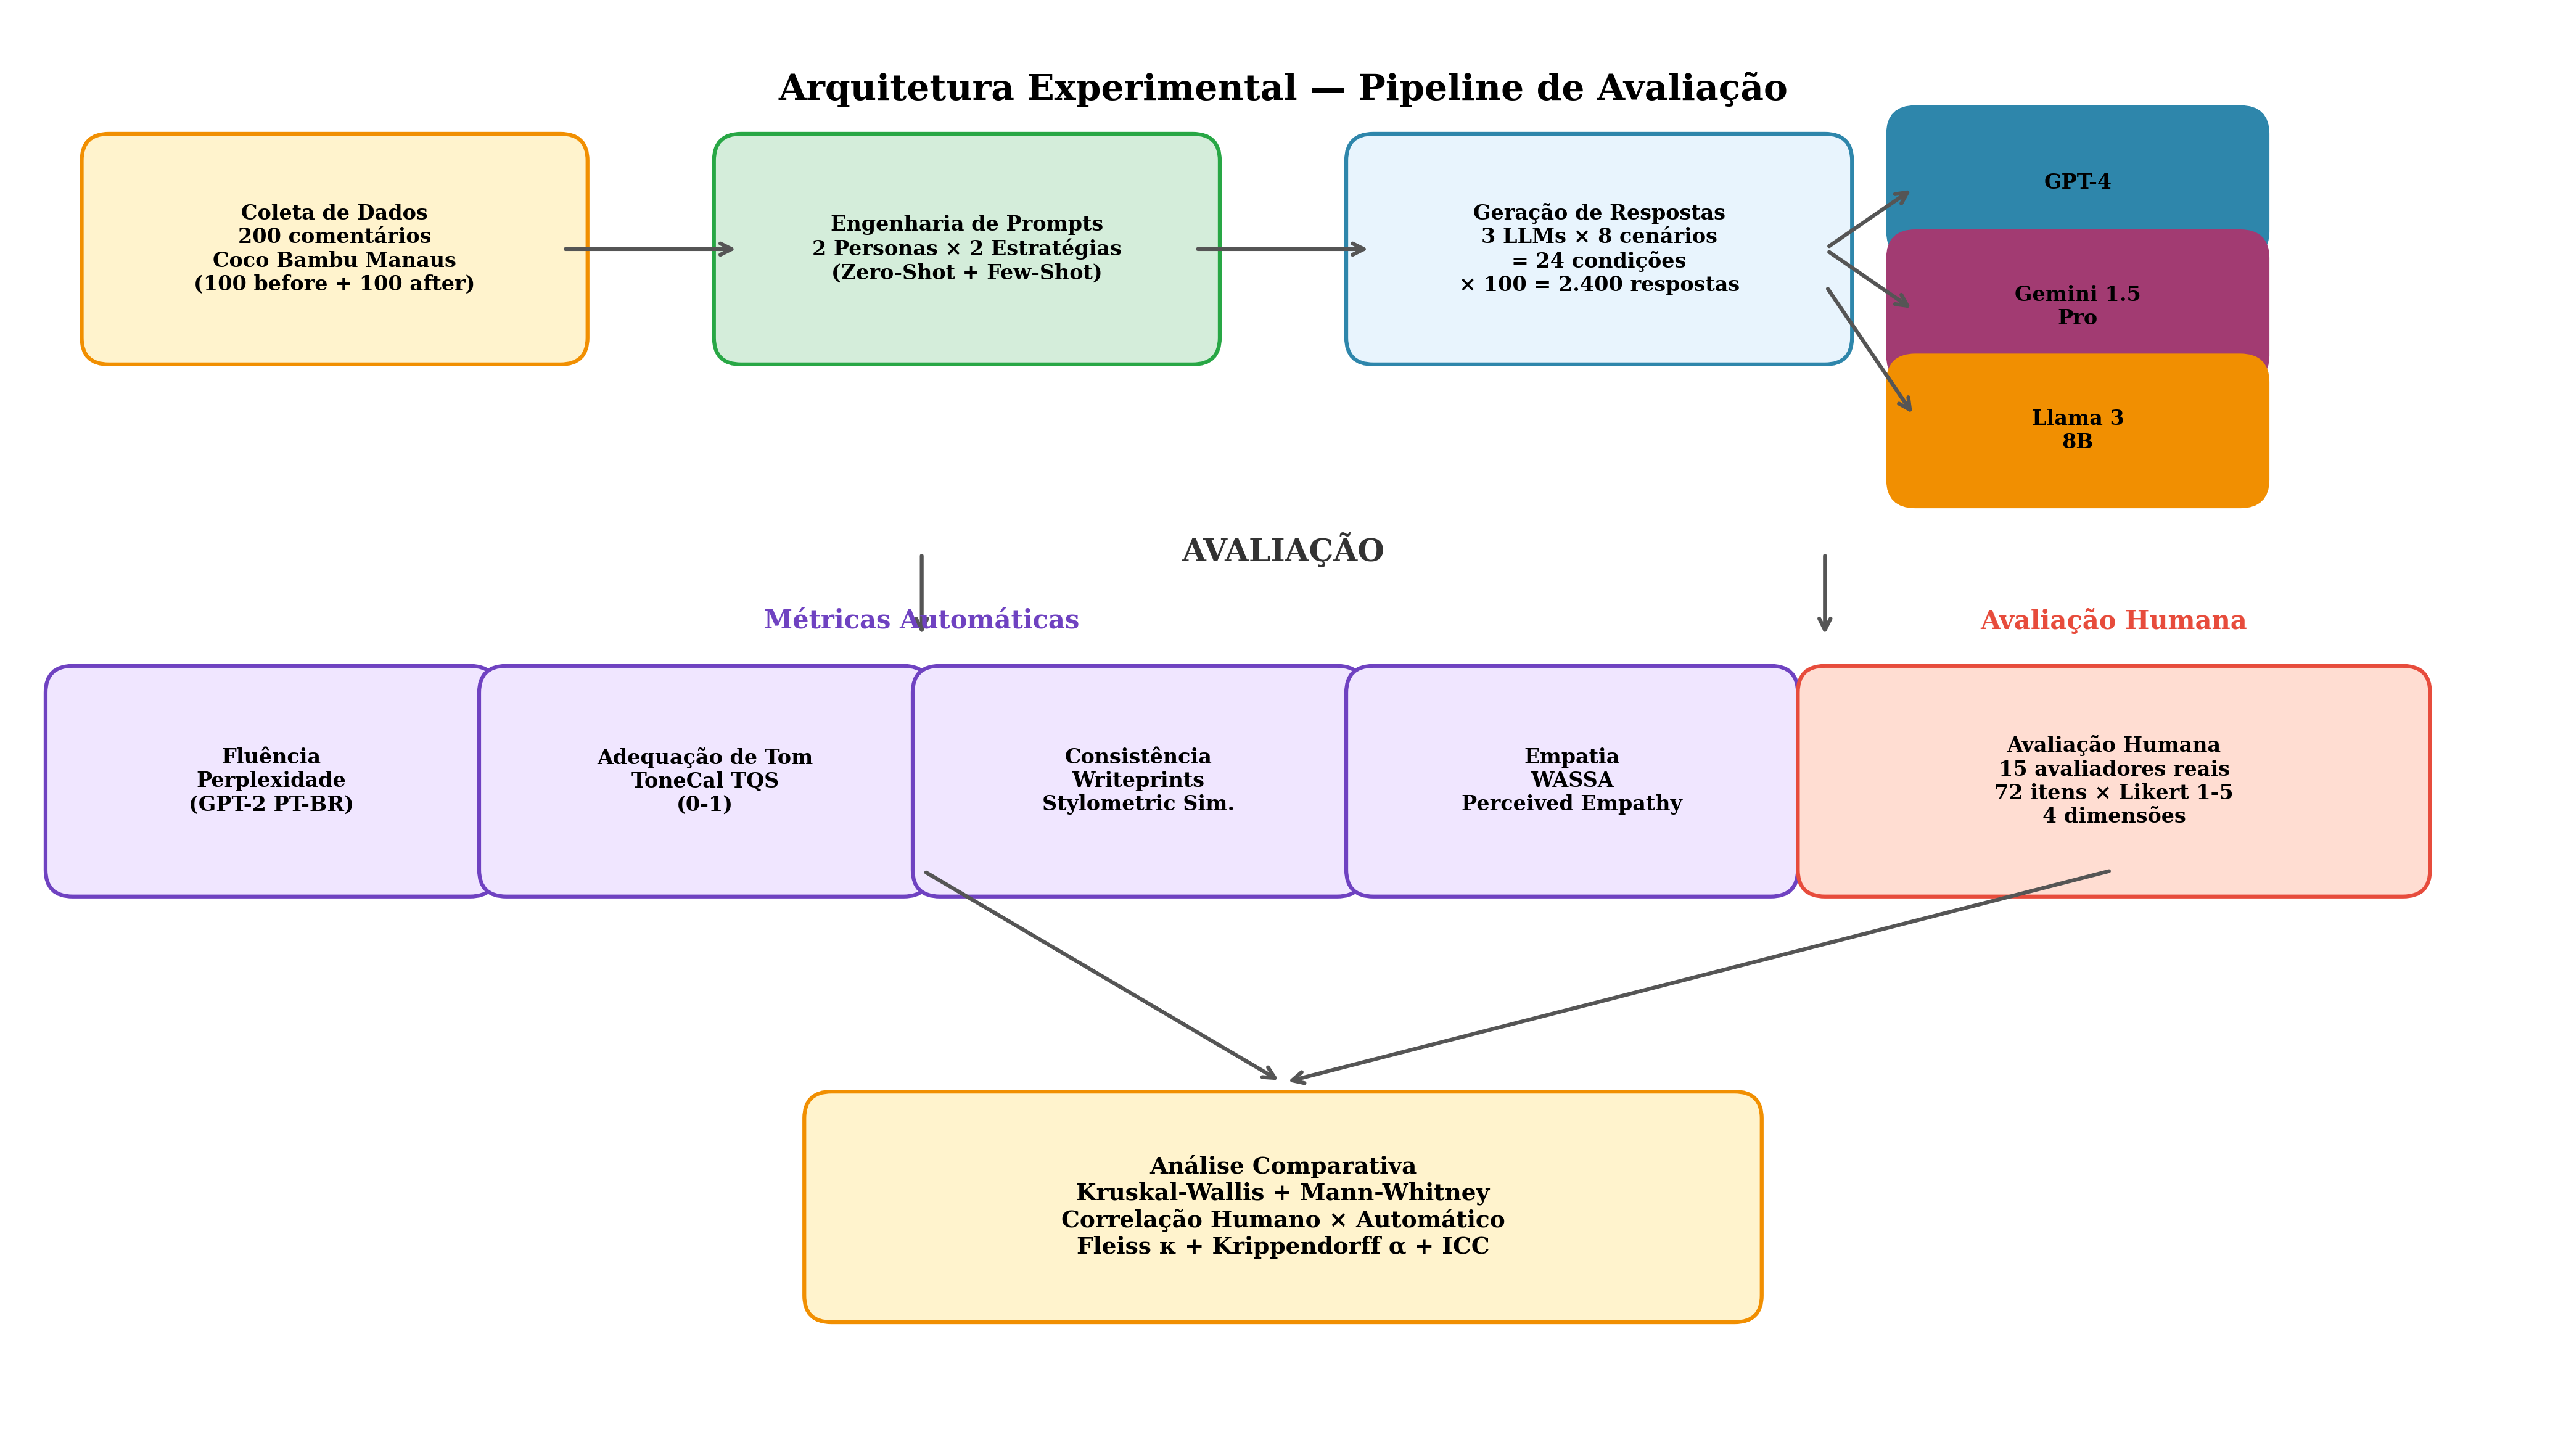
\includegraphics[width=1.0\linewidth]{img/arquitetura_experimental_tcc2.png}
    \caption{\textit{Coleta de 200 comentários, engenharia de \textit{prompts} com duas personas e duas estratégias, geração de 2.400 respostas por três \textit{LLMs}, e avaliação multidimensional com análise comparativa.}}
    \label{fig:fig_arq_1}
\end{figure}

\subsection{Conjunto de Dados}

O conjunto de dados utilizado nesta pesquisa é composto por duas partes principais: o \textit{Corpus de Origem}, que consiste nos comentários reais coletados, e o \textit{Corpus Resultante}, que compreende as respostas automáticas produzidas pelos \textit{LLMs} durante o \textit{pipeline} experimental.

\subsubsection{Corpus de Origem e Marco Temporal}

O \textit{Corpus de Origem} é formado por um total de 200 comentários reais de clientes, todos em língua portuguesa, coletados de plataformas digitais como \textit{Google Maps, TripAdvisor e Instagram}.

Uma decisão metodológica crucial para a integridade deste estudo foi a definição de um marco temporal rígido para a coleta dos dados, estabelecido em \textit{30 de novembro de 2022}, data oficial de lançamento do \textit{ChatGPT} pela \textit{OpenAI}. A divisão do corpus em dois períodos distintos justifica-se pela necessidade de garantir uma \textit{baseline} puramente humana:

\begin{itemize}
    \item \textit{{Período Pré-LLMs (Antes de 30/11/2022)}}: Contém 100 comentários e respostas publicados antes desta data. Este subconjunto é vital para o estudo pois pode nos dar alguma certeza de que as respostas dadas pelos estabelecimentos foram redigidas por seres humanos, sem a assistência de ferramentas de IA generativa acessíveis. Ele serve como o "padrão-ouro" da resposta humana natural.

    \item \textit{{Período Pós-LLMs (Após 30/11/2022)}}: Contém 100 comentários publicados após a popularização das ferramentas. Embora estes comentários sejam reais, eles representam o cenário atual onde a interação digital já está inserida em um contexto de maior volume e rapidez.
\end{itemize}

Essa separação impede a contaminação da amostra de controle, assegurando que não estamos comparando "IA contra IA", mas sim "IA contra Humanos".

\subsubsection{Uso do corpus como referência humana nas métricas automáticas.}
\label{subsec:corpus_origem}
 A separação entre os períodos pré e pós-popularização das \textit{LLMs} sustenta a análise comparativa descrita acima. No entanto, para a métrica de Similaridade Estilométrica(\textit{Writeprints}), que demanda um perfil agregado da \textit{voz} da marca, optou-se por compor a referência humana a partir do conjunto completo das 200 respostas originais do restaurante, tanto do período pré quanto do pós-popularização das \textit{LLMs}. Esta decisão metodológica baseia-se em duas justificativas: 
 \begin{itemize}
     \item A métrica estilométrica captura padrões agregados de estilo (distribuição lexical, complexidade sintática, padrões de pontuação e \textit{n-gramas}) que caracterizam a identidade comunicacional da marca como um todo, independentemente da autoria individual de cada resposta;
     \item  A ampliação da base de referência aumenta a estabilidade estatística do perfil estilométrico extraído, reduzindo o impacto de variações características  presentes em amostras reduzidas.
 \end{itemize} 
 Reconhece-se, contudo, que respostas do período pós-popularização das \textit{LLMs} podem ter sido elaboradas com auxílio de ferramentas de IA generativa, o que constitui uma limitação inerente ao uso de dados públicos contemporâneos. Para as demais métricas (Avaliação Humana, Perplexidade, \textit{ToneCal e WASSA}), que avaliam cada resposta gerada de forma independente, esta consideração não se aplica, pois não há comparação direta com uma referência humana específica.

\textit{\subsubsection{Corpus Resultante}}

O \textit{Corpus Resultante} é o principal resultado do \textit{Pipeline} Experimental da arquitetura. A partir dos 200 comentários do \textit{Corpus de Origem}, foi gerado um conjunto de 2.400 respostas automáticas.

Este conjunto de dados foi estruturado em torno de quatro eixos experimentais para permitir uma análise comparativa robusta:

\begin{itemize}
\item{\textit{Modelos de LLM}}: Para cada comentário, foram geradas respostas de três modelos distintos: \textit{Gemini 3.1}, \textit{GPT-5.5} e \textit{Llama 4}.

\item{\textit{Estratégia de Prompt}}: Duas técnicas de engenharia de \textit{prompt} foram aplicadas:

\subitem\textit{{Zero-Shot}}: A \textit{LLM} recebeu uma instrução direta sem exemplos prévios.

\subitem\textit{{Few-Shot}}: A \textit{LLM} recebeu a instrução acompanhada de alguns exemplos de respostas ideais.

\item\textit{{Persona da Marca}}: Duas \textit{personas} distintas foram definidas para avaliar a consistência de marca, conforme informado:

\subitem\textit{{Persona 1}}: Sofisticada e formal.

\subitem\textit{{Persona 2}}: Acolhedora e informal.

\item\textit{{Período temporal}}: O experimento foi aplicado a ambos os subconjuntos do \textit{Corpus de Origem} \textit{(Antes das LLMs e Depois das LLMs)}.
\end{itemize}

Essa estrutura resulta em 8 arquivos de dados gerados:
\begin{itemize}
\item\textit{After-Llm-Release-Comments-Generated-Responses-Persona-1-Few-Shot}

\item\textit{After-Llm-Release-Comments-Generated-Responses-Persona-1-Zero-Shot}

\item\textit{After-Llm-Release-Comments-Generated-Responses-Persona-2-Few-Shot}

\item\textit{After-Llm-Release-Comments-Generated-Responses-Persona-2-Zero-Shot}

\item\textit{Before-Llm-Comments-Generated-Responses-Persona-1-Few-Shot}

\item\textit{Before-Llm-Comments-Generated-Responses-Persona-1-Zero-Shot}

\item\textit{Before-Llm-Comments-Generated-Responses-Persona-2-Few-Shot}

\item\textit{Before-Llm-Comments-Generated-Responses-Persona-2-Zero-Shot}
\end{itemize}

Cada um desses 8 arquivos contém 100 linhas que apresentam o comentário gerado pela devida \textit{LLM (Gemini, GPT, Llama)} para aquela condição específica (ex: Período \textit{"After"}, \textit{Persona} "Sofisticada", Estratégia \textit{"Few-shot"}).

A Tabela~\ref{tab:generated_csv_file} demonstra a estrutura padronizada dentro dos arquivos com as respostas geradas.

\begin{table}[H]
\centering
\small
\resizebox{\textwidth}{!}{%
\begin{tabular}{|c|c|c|c|c|c|}
\hline
\rowcolor[HTML]{9B9B9B}
\textit{GPT-5.5 \textit{"{Persona}"}} & \textit{Gpt \textit{Processing Time}} & \textit{Gemini 3.1 \textit{"{Persona}"}} & \textit{Gemini \textit{Processing Time}} & \textit{Llama 4 \textit{"{Persona}"}} & \textit{Llama \textit{Processing Time}} \\ \hline

"Comentário gerado" & "X segundos" & "Comentário gerado" & "X segundos" & "Comentário gerado" & "X segundos" \\ \hline

"Comentário gerado" & "X segundos" & "Comentário gerado" & "X segundos" & "Comentário gerado" & "X segundos" \\ \hline

"Comentário gerado" & "X segundos" & "Comentário gerado" & "X segundos" & "Comentário gerado" & "X segundos" \\ \hline

"Comentário gerado" & "X segundos" & "Comentário gerado" & "X segundos" & "Comentário gerado" & "X segundos" \\ \hline

\end{tabular}%
}
\caption{Comparativo de Adequação de Persona e Tempo de Processamento por LLM}
\label{tab:generated_csv_file}
\end{table}

A Tabela~\ref{tab:dataset_summary} resume a estrutura do conjunto de dados gerado.

\begin{table}[H]
\centering
\small
\resizebox{\textwidth}{!}{%
\begin{tabular}{|c|c|}
\hline
\rowcolor[HTML]{9B9B9B}
\textit{Eixo Experimental} & \textit{Variáveis} \\ \hline
Comentários-Fonte & 200 (100 antes, 100 depois) \\ \hline
Modelos \textit{LLM} & 3 (\textit{Gemini, GPT, Llama}) \\ \hline
Personas & 2 (Sofisticada e Formal, Acolhedora e Informal) \\ \hline
Estratégias de \textit{Prompt} & 2 \textit{(Zero-Shot, Few-Shot)} \\ \hline
\textit{Total de Respostas Geradas} & \textit{2.400 (200 $\times$ 3 $\times$ 2 $\times$ 2 )} \\ \hline
\end{tabular}%
}
\caption{Resumo da Estrutura do Conjunto de Dados Gerado}
\label{tab:dataset_summary}
\end{table}
 
O cruzamento completo dos quatro eixos experimentais, 3 modelos $\times$ 2 personas 
$\times$ 2 estratégias $\times$ 2 períodos, define 24 cenários experimentais 
únicos. Cada cenário corresponde a uma combinação específica (e.g., \textit{GPT-5.5} + Persona 
Sofisticada + \textit{Zero-Shot} + Período \textit{After}) e contém 100 respostas geradas 
(uma por comentário do corpus de origem). Essa estrutura fatorial completa permite isolar 
o efeito de cada variável independente sobre a qualidade das respostas.

\subsubsection{Considerações Éticas e Tratamento dos Dados}
\label{subsec:consideracoes_eticas}
A presente pesquisa foi conduzida com observância dos princípios éticos aplicáveis ao tratamento de dados textuais coletados em plataformas digitais públicas. Todos os comentários que compõem o \textit{Corpus de Origem} foram extraídos de \textit{reviews} disponibilizados publicamente pelos próprios autores em plataformas como \textit{Google Maps}, \textit{TripAdvisor} e \textit{Instagram}, nas quais os usuários, ao publicarem suas avaliações, consentem com a visibilidade pública do conteúdo.
Os dados foram tratados de forma anonimizada, com remoção ou ocultação de nomes de usuários, fotografias de perfil, identificadores de conta, \textit{URLs} associadas e quaisquer outros elementos suscetíveis à identificação direta dos autores. As capturas de tela e exemplos textuais apresentados ao longo deste trabalho foram utilizados exclusivamente para fins acadêmicos de ilustração metodológica, tendo informações sensíveis sistematicamente mascaradas. Eventuais nomes próprios mencionados no corpo dos comentários (e.g., nomes de funcionários do estabelecimento citados em elogios ou críticas) foram preservados na forma original quando integrantes do registro público de avaliações, sem qualquer juízo de valor ou exposição adicional por parte da pesquisa.

Os dados não foram empregados para fins comerciais, perfilamento individual ou qualquer aplicação que extrapole o escopo acadêmico-científico aqui descrito. O tratamento adotado observa os princípios de finalidade, necessidade e transparência previstos na Lei Geral de Proteção de Dados (\textit{LGPD}, Lei n.\ 13.709/2018), tratando os comentários como dados pessoais de natureza pública divulgados pelo próprio titular, com uso restrito ao interesse legítimo de pesquisa científica. O \textit{Corpus de Origem} e o \textit{Corpus Resultante} disponibilizados no repositório do projeto (Apêndice~\ref{apendice:repositorio}) seguem o mesmo procedimento de anonimização adotado neste documento, assegurando que sua reutilização em trabalhos futuros preserve os princípios éticos aqui descritos.

\subsubsection{Uso Consciente de Inteligência Artificial Generativa}
\label{subsec:uso_consciente_ia}

Considerando que o objeto de estudo desta pesquisa são precisamente os \textit{Large Language Models}, registra-se de forma explícita e transparente que ferramentas de Inteligência Artificial generativa foram utilizadas como apoio em etapas auxiliares da elaboração deste trabalho. Esse uso seguiu princípios de transparência, supervisão crítica e responsabilidade autoral. A autoria intelectual, conceitual e científica do trabalho permanece exclusivamente do autor, com orientação acadêmica institucional. Nenhuma ferramenta de \textit{IA} é creditada como coautora, em alinhamento com as diretrizes editoriais correntes em periódicos científicos sobre o uso responsável de \textit{IA} na pesquisa.

Especificamente, recursos de \textit{IA} generativa foram empregados como assistentes nas seguintes atividades auxiliares: 

\begin{itemize}
\item Revisão ortográfica, padronização de acentuação e uniformização de termos técnicos ao longo do documento, com validação final realizada pelo autor; 

\item Geração de \textit{scripts} de visualização de dados em \textit{Python} (\textit{boxplots}, gráficos de dispersão, gráfico polar e barras comparativas), todos posteriormente revisados, executados e validados quanto à correção dos dados representados;

\item Apoio à pesquisa bibliográfica, com sugestões iniciais de literatura potencialmente relevante, sendo cada referência verificada manualmente quanto à existência, à fidelidade da citação e à pertinência ao argumento desenvolvido;

\item Apoio à concepção visual de figuras e diagramas conceituais, incluindo sugestões de paleta de cores, \textit{layout} e organização de elementos, sob direção editorial integral do autor.
\end{itemize}

De maneira igualmente importante, registra-se que ferramentas de \textit{IA} generativa \textit{não} foram utilizadas nas seguintes atividades centrais à pesquisa:

\begin{itemize}

\item Coleta de dados, realizada manualmente nas plataformas \textit{Google Maps}, \textit{TripAdvisor} e \textit{Instagram};

\item Geração das respostas avaliadas, que constituem o próprio objeto de estudo e não foram revisadas ou pós-processadas por \textit{IA} antes da avaliação; 

\item Análise estatística, incluindo os testes de \textit{Kruskal-Wallis}, \textit{Mann-Whitney~U}, \textit{Fleiss}~$\kappa$, \textit{Krippendorff}~$\alpha$ e \textit{ICC}, conduzidos pelo autor sem assistência de \textit{IA};

\item Decisões metodológicas, formulação de hipóteses de pesquisa e interpretação dos resultados, integralmente de autoria humana.

\end{itemize}

Toda saída produzida com apoio de \textit{IA} passou por revisão crítica do autor, que assume responsabilidade integral pelo conteúdo final apresentado neste documento.

\subsection{Métricas de Avaliação}

A avaliação da qualidade de textos gerados por \textit{LLMs} é uma tarefa intrinsecamente complexa, especialmente ao tentar mensurar variáveis subjetivas como tom, empatia, fluência e consistência de marca. A literatura acadêmica aponta que não há uma métrica automática singular capaz de capturar a totalidade da adequação direta e da percepção humana em tarefas de geração de linguagem natural~\cite{howcroft2020twenty}.

Por essa razão, este trabalho emprega uma metodologia mista, alinhada com os objetivos da pesquisa. Esta abordagem combina uma rigorosa avaliação humana qualitativa, considerada o \textit{"padrão-ouro" (gold standard)} para este tipo de tarefa~\cite{celikyilmaz2021Evaluation}, com métricas quantitativas automáticas para objetividade e escalabilidade.

\subsubsection{Avaliação Humana (Qualitativa)}

A principal forma de avaliação adotada neste estudo é qualitativa, fundamentada em julgamento humano. Reconhecendo que a clientela de restaurantes é intrinsecamente heterogênea, a composição da banca de avaliadores foi desenhada estrategicamente para evitar vieses de bolhas tecnológicas ou geracionais.

Foram selecionados 15 avaliadores independentes, com idades entre 21 e 71 anos (média de 40 anos), distribuídos em quatro faixas etárias para assegurar representação intergeracional: quatro avaliadores entre 21 e 29 anos, cinco entre 30 e 39 anos, quatro entre 40 e 59 anos e dois com 60 anos ou mais. Quanto à atuação profissional, o painel reuniu perfis heterogêneos: quatro profissionais da área da saúde (dois médicos, um dentista e um profissional de educação física), quatro engenheiros (dois engenheiros de \textit{software}, um engenheiro florestal e um engenheiro elétrico), três estudantes universitários, uma advogada, um corretor de imóveis e dois avaliadores em situação ocupacional distinta (uma autônoma e um aposentado). Essa composição contempla diferentes níveis de letramento digital e familiaridade com tecnologias de \textit{IA}, bem como diferentes contextos de consumo gastronômico, mitigando vieses de percepção associados a bolhas tecnológicas, ocupacionais ou geracionais e aproximando o painel da heterogeneidade da clientela real de restaurantes~\cite{howcroft2021}.

Cada avaliador analisou um conjunto cego de 72 itens (respostas geradas), selecionados por amostragem estratificada proporcional: 3 itens por cenário experimental ($3 \times 24$ cenários $= 72$), garantindo representação de todas as combinações de modelo, persona, estratégia e período. A seleção dentro de cada cenário foi realizada por subamostragem aleatória dentre as 100 respostas disponíveis naquele estrato, assegurando cobertura sistemática do espaço experimental. Os itens foram apresentados sem identificação do modelo de origem, utilizando um \textit{Scorecard} (Apêndice~\ref{apendice:formulario_completo}) com escala \textit{Likert} de 5 pontos para quatro dimensões: Empatia, Consistência de Marca, Adequação de Tom e Fluência.

A concordância inter-avaliadores foi aferida por três coeficientes complementares (cf.\ Seção~\ref{subsec:metricas_avaliacao_ft}): \textit{Fleiss' Kappa} ($\kappa$), que mede a concordância nominal além do acaso; \textit{Krippendorff's Alpha} ($\alpha$) com ponderação ordinal, que leva em conta a magnitude das discordâncias; e o \textit{Intraclass Correlation Coefficient} (ICC\textsubscript{2,1}), que avalia a consistência absoluta entre avaliadores tratados como efeito aleatório. Os valores obtidos, $\kappa$ entre 0,76 e 0,86 (substancial a quase perfeita), $\alpha$ entre 0,82 e 0,94, e ICC entre 0,88 e 0,94, atestam a robustez e a reprodutibilidade dos julgamentos humanos coletados.

A Figura~\ref{fig:diagrama_avaliacao_humana} ilustra o processo completo de avaliação humana adotado neste estudo.

\begin{figure}[H]
\centering
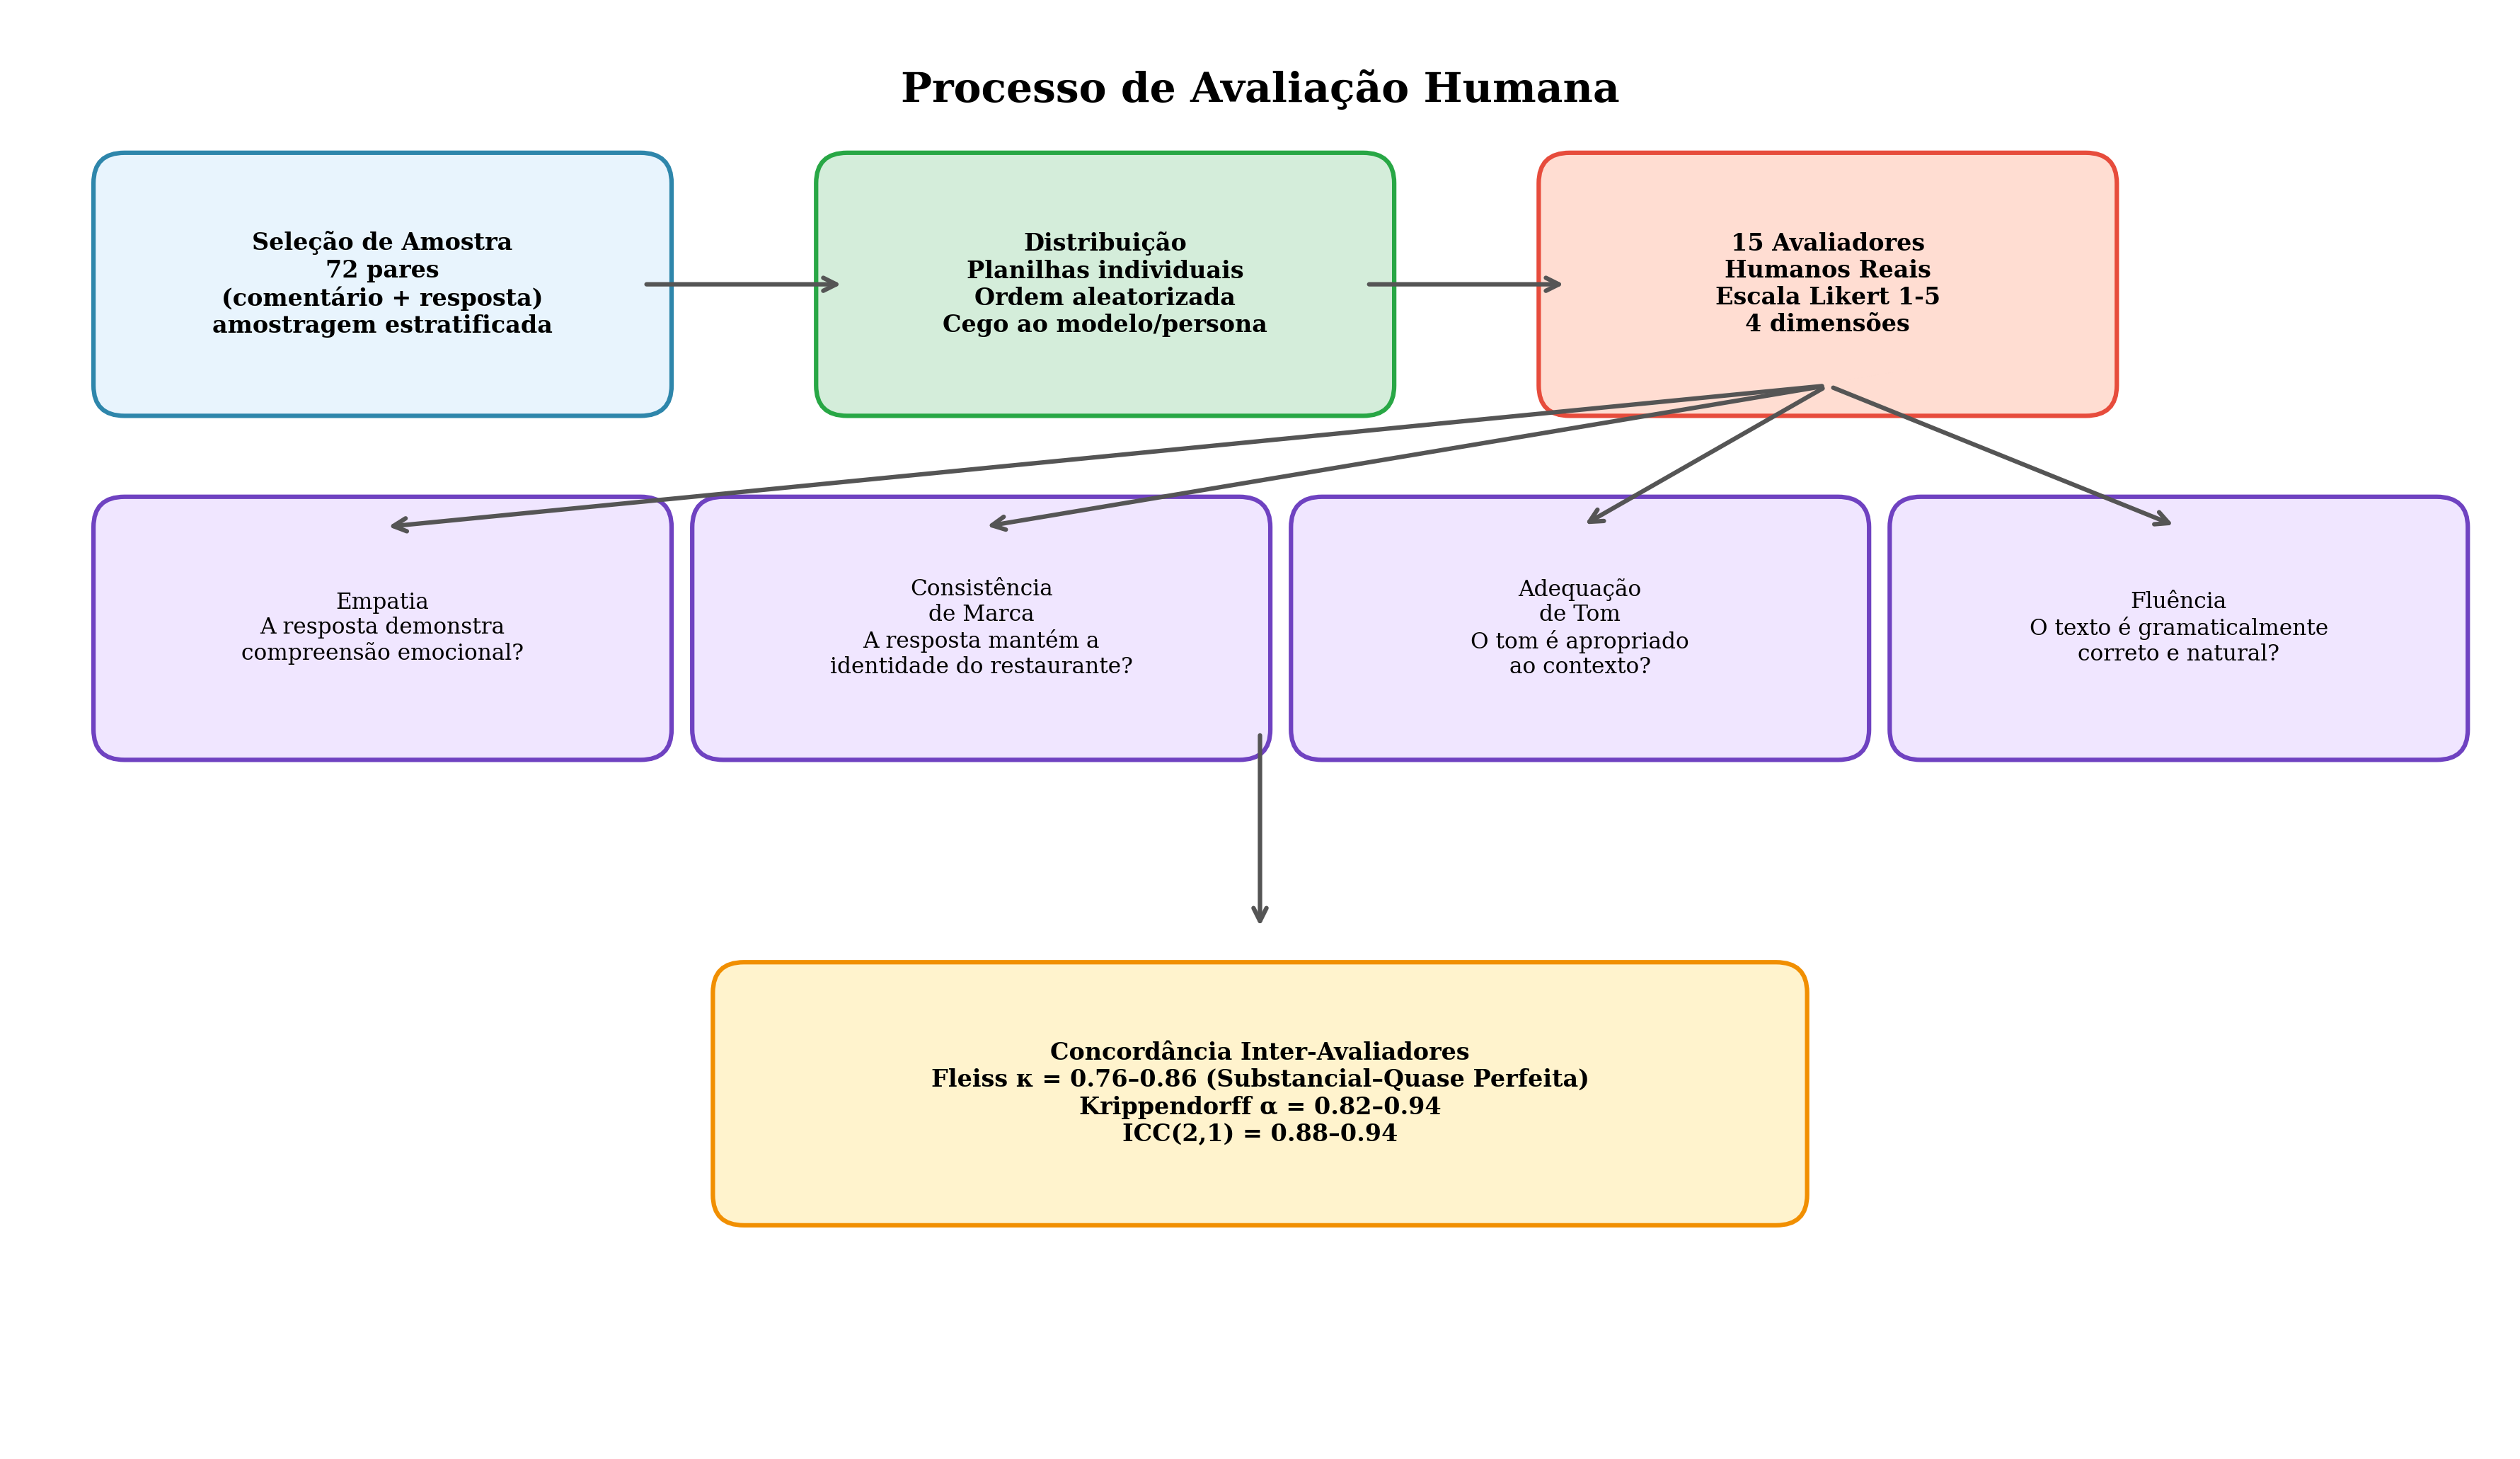
\includegraphics[width=\textwidth]{img/diagrama_avaliacao_humana.png}
\caption{72 pares comentário-resposta selecionados por amostragem estratificada, distribuídos individualmente com ordem aleatorizada e cegamento ao modelo. Os 15 avaliadores avaliaram quatro dimensões em escala Likert 1--5, com concordância inter-avaliadores de $\kappa = 0{,}76$--$0{,}86$ (Fleiss).}
\label{fig:diagrama_avaliacao_humana}
\end{figure}

\subsubsection{Avaliação Automática (Quantitativa)}

Para complementar a avaliação humana com objetividade e escalabilidade, foi empregado um \textit{framework} de quatro métricas automáticas, cada uma capturando uma dimensão distinta da qualidade textual. Esta abordagem multimétrica alinha-se à recomendação de \citeonline{liang2023} por avaliações holísticas que transcendam uma métrica agregada.

\paragraph{Fluência Textual --- Perplexidade (GPT-2 PT-BR).}
A fluência das respostas geradas foi aferida por meio da perplexidade (\textit{PPL}), calculada com o modelo \textit{GPT-2} pré-treinado para o português brasileiro (\textit{pierreguillou/gpt2-small-portuguese}). Formalmente, para uma sequência de \textit{tokens} $w_1, w_2, \ldots, w_N$:

\begin{equation}
PPL(w_1, \ldots, w_N) = \exp \left( -\frac{1}{N} \sum_{i=1}^{N} \log P(w_i \mid w_1, \ldots, w_{i-1}) \right)
\label{eq:perplexity}
\end{equation}

A perplexidade mede a fluência \textit{probabilística} do texto, quantificando a previsibilidade do próximo \textit{token} dado o contexto precedente. Seus valores devem ser interpretados como \textit{proxy} de naturalidade linguística, considerando que textos formais e mais longos tendem a obter valores mais baixos independentemente da qualidade pragmática.

\paragraph{Adequação de Tom --- ToneCal (TQS).}
A adequação de tom foi avaliada pela métrica \textit{ToneCal} (\textit{Tone Quality Score}), na escala $[0, 1]$, implementada com base no \textit{framework} de polidez de \citeonline{danescu2013} e na sistematização de \citeonline{priya2024}. A métrica opera sobre marcadores lexicais de superfície, saudações, expressões de deferência, escolha de modo verbal e indicadores de cortesia, sendo mais sensível a indicadores explícitos de polidez do que a nuances pragmáticas de tom implícito. Neste estudo, o ToneCal analisa marcadores de cortesia, deferência e assertividade contextualizada, calibrados para as duas personas de atendimento definidas (Tabela~\ref{tab:dataset_summary}).

\paragraph{Consistência de Marca --- Similaridade Estilométrica (\textit{Writeprints}).}
A consistência de marca foi mensurada por similaridade estilométrica via \textit{Writeprints}~\cite{abbasi2008}. A implementação extrai perfis multidimensionais (distribuição lexical, complexidade sintática, frequência de \textit{n-gramas} de caracteres e padrões de pontuação) do corpus de referência humano (200 respostas originais do restaurante) e de cada resposta gerada, computando a similaridade na escala $[0, 1]$. Conforme detalhado  na  Seção~\ref{subsec:corpus_origem}, o perfil estilométrico de referência foi extraído do conjunto  completo das 200 respostas humanas do restaurante.

\paragraph{Empatia Percebida --- Modelo WASSA.}
A empatia percebida foi aferida pelo modelo treinado na \textit{WASSA Shared Task}~\cite{barriere2023}, produzindo pontuações na escala $[1, 5]$. Embora o modelo original tenha sido desenvolvido em inglês para o domínio jornalístico, sua arquitetura baseada em \textit{transformers} multilíngues permite a captura de padrões empáticos transferíveis entre línguas e domínios~\cite{barriere2023}. Neste estudo, a métrica é empregada como indicador comparativo entre modelos e estratégias, permitindo identificar diferenças relativas nos níveis de empatia das respostas geradas.

\subsection{\textit{Large Language Models}}

A seleção dos modelos para este estudo (Objetivo Específico 4) foi pautada na necessidade de avaliar o desempenho do atual estado da arte em geração de linguagem, abrangendo os principais exemplares de \textit{LLMs} disponíveis~\cite{zhao2023Survey}. O objetivo é avaliar a viabilidade e maturidade dessas ferramentas para o contexto de restaurantes.

Para realizar uma análise comparativa robusta, foram selecionados três modelos de ponta que representam as duas principais vertentes do ecossistema de \textit{LLMs}: os modelos proprietários (fechados) e os modelos de pesos abertos \textit{(open-weight)}.

A escolha específica dos modelos \textit{GPT-5.5}, \textit{Gemini 3.1} e \textit{Llama 4} permite a este estudo cobrir o que há de mais avançado em cada uma dessas vertentes:

\begin{itemize}

\item \textit{GPT-5.5 (OpenAI):} Selecionado por ser amplamente considerado o \textit{benchmark} da indústria em termos de capacidade de raciocínio, geração de texto e, crucialmente, seguimento de instruções complexas (como as de persona e tom)~\cite{Minaee2025Survey}. Sua performance é frequentemente utilizada como a linha de base (\textit{baseline}) para o que é considerado o estado da arte, sendo essencial para estabelecer o teto de performance esperado para a tarefa.

\item \textit{Gemini 3.1 (Google):} Incluído como o principal competidor do \textit{GPT-5.5}. Os modelos da família \textit{Gemini} têm demonstrado capacidades de ponta, nativamente multimodais e com forte compreensão de contexto~\cite{google2024gemini}. Sua inclusão permite uma comparação direta entre as duas \textit{LLMs} de grande escala mais proeminentes no mercado, avaliando qual delas oferece melhor adequação para a geração de respostas empáticas.

\item \textit{Llama 4 (Meta):} Representa o estado da arte dos modelos de pesos abertos \textit{(*open-weight*)}. O \textit{Llama 4}, especificamente, foi treinado em um conjunto de dados massivo e diverso, com melhorias notáveis em seu \textit{tokenizador} para abranger de forma mais eficiente múltiplas línguas, incluindo o português~\cite{meta2024llama3}. Sua inclusão é vital para responder uma questão chave da pesquisa: se soluções \textit{open-source}, que oferecem maior controle e possibilidade de \textit{fine-tuning}, já atingem um nível de maturidade comparável ao dos modelos proprietários em tarefas de alta nuance, como as definidas neste trabalho.

\end{itemize}

Um pilar central deste estudo é o foco exclusivo na língua portuguesa. Conforme discutido na Fundamentação Teórica (Seção 2.2), o desempenho de modelos multilíngues pode variar, e o pré-treinamento monolíngue (ou com forte representação do idioma) pode capturar melhor as nuances culturais e linguísticas~\cite{araujo2024Explorando}.

Portanto, no sentido prático da metodologia e alinhado à arquitetura experimental (Figura~\ref{fig:fig_arq_1}), esta seleção foi implementada da seguinte forma: para cada um dos 200 comentários do \textit{Corpus de Origem}, os \textit{prompts} (descritos na Seção 4.5) foram formatados e submetidos programaticamente aos modelos.

Para os modelos proprietários, \textit{GPT-5.5 e Gemini 3.1}, a interação foi realizada através de suas respectivas \textit{APIs} oficiais.

Cada resposta textual gerada foi então sistematicamente coletada e armazenada no \textit{Corpus Resultante} (Tabela~\ref{tab:generated_csv_file}). Este processo permitiu a avaliação comparativa direta da performance bruta (tempo de processamento) e da adequação qualitativa (naturalidade, empatia, consistência de marca) de cada arquitetura no contexto específico do português brasileiro. O código-fonte completo da implementação está disponível no Apêndice~\ref{apendice:repositorio}.

 \subsection{Parâmetros e Procedimento de Geração}
 
 A execução experimental foi conduzida de forma programática, em ambiente \textit{Python}, com chamadas sequenciais aos três modelos avaliados. Para cada um dos 200 comentários do \textit{Corpus de Origem}, o \textit{prompt} estruturado (descrito na 
Seção~\ref{subsec:prompts_empregados}) foi submetido a cada modelo (\textit{GPT-5.5}, 
\textit{Gemini 3.1} e \textit{Llama 4}), combinando-se as duas personas e as duas estratégias de \textit{prompting}, totalizando os 24 cenários experimentais e as 2.400 respostas que compõem o \textit{Corpus Resultante}.
 
Os modelos proprietários (\textit{GPT-5.5} e \textit{Gemini 3.1}) foram acessados por meio de suas \textit{APIs} oficiais, enquanto o modelo de pesos abertos \textit{Llama 4} foi executado em ambiente local controlado, garantindo a reprodutibilidade integral do procedimento.

A fim de promover variabilidade lexical suficiente sem comprometer a coerência das respostas, adotou-se o parâmetro de temperatura igual a 0{,}7 em todos os modelos, valor intermediário entre a geração determinística (\textit{T = 0}) e a geração altamente estocástica (\textit{T = 1}), comumente empregado em tarefas criativas de geração textual em linguagem natural\cite{holtzman2020, peeperkorn2024, renze2024}.
 
 Os demais parâmetros de \textit{decoding} foram mantidos nos valores padrão das respectivas 
implementações, especificamente o \textit{top-p} (\textit{nucleus sampling}) e o limite máximo de 
\textit{tokens} de saída. Esta decisão visou preservar o comportamento nativo de cada arquitetura 
e permitir uma comparação metodologicamente justa entre os modelos, evitando que ajustes finos 
privilegiassem injustificadamente uma das vertentes avaliadas. O controle da extensão das 
respostas foi efetuado por meio de instrução explícita no \textit{prompt} (entre duas e quatro 
frases), assegurando respostas dentro da extensão típica de interações em plataformas de 
\textit{review}.
 
 Cada chamada gerou uma única resposta, registrada juntamente com seu respectivo tempo de 
processamento. Não foram aplicados mecanismos de regeneração automática nem critérios de descarte 
seletivo: todas as 2.400 saídas produzidas foram preservadas e submetidas integralmente às etapas 
posteriores de avaliação. Esta escolha metodológica evita vieses de seleção \textit{a posteriori} 
e assegura que os resultados reflitam o comportamento real de cada modelo na tarefa proposta. O 
código-fonte completo, os \textit{prompts} empregados e os dados utilizados encontram-se 
disponíveis no repositório indicado no Apêndice~\ref{apendice:repositorio}.

\subsection{\textit{Prompts} Empregados}
\label{subsec:prompts_empregados}

O desenvolvimento dos \textit{prompts} (Objetivo Específico 2) é um pilar central desta metodologia. Os \textit{prompts} não são apenas a entrada, mas o principal instrumento de controle experimental usado para guiar as \textit{LLMs} na geração de respostas que se alinhem às variáveis de análise (tom, empatia, fluência e consistência de marca)~\cite{mello2024prompt}.

Conforme a estrutura do \textit{Corpus Resultante} (Seção 4.2.2), o experimento foi desenhado para comparar duas estratégias de \textit{prompt} sobre duas personas distintas. Para isso, foi estabelecida uma estrutura de \textit{"prompt base"} que, então, foi adaptada para as duas condições experimentais: \textit{Zero-Shot} e \textit{Few-Shot}.


\subsubsection{Estrutura Base do \textit{Prompt} (Componente Fixo)}

Todos os \textit{prompts} utilizados, independentemente da estratégia (\textit{Zero-Shot} ou \textit{Few-Shot}), compartilharam uma estrutura base arquitetada para padronizar o comportamento do modelo antes da inserção de quaisquer exemplos. Baseada em técnicas de engenharia de \textit{prompt}~\cite{Mesko2023Prompt}, esta estrutura fixa continha os seguintes componentes:

\begin{itemize}
 \item Atribuição de Papel: A instrução inicial ancora a identidade da \textit{LLM} (ex: "Você é o gerente do \textit{Instagram}...") e define a \textit{persona} específica a ser adotada (Acolhedora ou Sofisticada), estabelecendo o viés comportamental da resposta.

 \item Definição da Tarefa e Tom: Uma descrição concisa do objetivo ("responder ao Comentário do Cliente") combinada com uma diretriz de estilo explícita ("tom compreensivo e empático"), garantindo que a modulação emocional seja priorizada.

\item Diretrizes Condicionais : Um bloco de regras lógicas que orienta a tomada de decisão do modelo com base na análise de sentimento do comentário. O \textit{prompt} instrui explicitamente como reagir a cenários distintos: oferecer desculpas e soluções em casos negativos, ou demonstrar alegria e exaltar a experiência em casos positivos/neutros.

 \item Restrições de Saída: Uma diretiva de formatação ("Não precisa demonstrar seu pensamento. Retorne apenas a resposta...") utilizada para impedir que o modelo gere metatexto, explicações ou cadeias de pensamento visíveis, assegurando que o \textit{output} seja estritamente a resposta final ao cliente.
\end{itemize}

\subsubsection{Estratégia Experimental 1: \textit{Prompt Zero-Shot}}

Na condição \textit{Zero-Shot}, o modelo recebe apenas a estrutura base do \textit{prompt} e o novo comentário do cliente. Nenhum exemplo de resposta é fornecido.

Esta abordagem testa a capacidade de "raciocínio em-contexto" \textit{(zero-shot reasoning)} da \textit{LLM}~\cite{kojima2022large}. O objetivo é avaliar a maturidade de cada modelo \textit{(GPT-5.5, Gemini, Llama 4)} para seguir instruções complexas e subjetivas (como "ser empático") sem qualquer treinamento prévio para a tarefa específica, baseando-se apenas em seu conhecimento pré-treinado~\cite{zhao2023Survey}. Esta condição serve como a (\textit{baseline}) do desempenho. A Figura~\ref{fig:template_zero_shot} apresenta o \textit{template} utilizado.
\newline
\newline
\newline
\newpage
\textit{Estrutura Prática \textit{(Template)}:}

\begin{figure}[H]
\centering
% Aumenta para 1.2x a largura da linha e centraliza
\makebox[\linewidth][c]{%

\includegraphics[width=0.8\linewidth]{img/zeroshot1.png}
}
\caption{\textit{Template do prompt} \textit{Zero-Shot}}
\label{fig:template_zero_shot}
\end{figure}

\subsubsection{Estratégia Experimental 2: \textit{Prompt Few-Shot}}

Na condição \textit{Few-Shot}, o \textit{prompt} é aumentado com a inclusão de exemplos de alta qualidade antes de apresentar o comentário a ser respondido.

\textit{Justificativa Metodológica:} Esta abordagem explora o \textit{In-Context Learning (ICL)}, onde o modelo aprende a tarefa a partir dos exemplos fornecidos no próprio \textit{prompt}~\cite{dang2022How}. O objetivo é medir o ganho de performance em relação à abordagem \textit{Zero-Shot}. Espera-se que, ao fornecer exemplos de como a persona e a empatia devem ser aplicadas na prática, a \textit{LLM} consiga gerar respostas mais alinhadas e consistentes, reduzindo a generalidade ou a "robotização" das respostas. A Figura~\ref{fig:template_few_shot} apresenta o \textit{template} utilizado.

\begin{figure}[H]
\centering
% Aumenta para 1.2x a largura da linha e centraliza
\makebox[\linewidth][c]{%

\includegraphics[width=0.8\linewidth]{img/fewshot1.png}
}
\caption{\textit{Template do prompt} \textit{Few-Shot}}
\label{fig:template_few_shot}
\end{figure}

A aplicação dessas duas estratégias (\textit{Zero-Shot e Few-Shot}) em todas as combinações de modelos e personas permitiu a criação sistemática das 2.400 respostas que compõem o \textit{Corpus Resultante}, possibilitando uma análise estatística e qualitativa robusta sobre qual abordagem é mais eficaz para a tarefa.

\newpage
\section{EXPERIMENTOS E RESULTADOS}

Esta seção apresenta a análise dos dados obtidos a partir das 2.400 respostas geradas, estratificadas pelos 24 cenários experimentais (3 modelos $\times$ 2 personas $\times$ 2 estratégias de \textit{prompt} $\times$ 2 períodos temporais). A avaliação integra os resultados da avaliação humana (15 avaliadores, 72 itens, escala \textit{Likert} 1--5) com as quatro métricas automáticas (Perplexidade, ToneCal, Similaridade Estilométrica e Empatia WASSA), visando uma análise multidimensional da qualidade das respostas.

\subsection{Concordância Inter-Avaliadores}

Antes de analisar os resultados da avaliação humana, é fundamental validar a confiabilidade dos julgamentos coletados. A Tabela~\ref{tab:concordancia} apresenta as métricas de concordância inter-avaliadores para cada dimensão avaliada.

\begin{table}[H]
\centering
\caption{Concordância Inter-Avaliadores por Dimensão (15 avaliadores, 72 itens)}
\label{tab:concordancia}
\begin{tabular}{@{}lccc@{}}
\toprule
\textbf{Dimensão} & \textbf{Fleiss' $\kappa$} & \textbf{Krippendorff's $\alpha$} & \textbf{ICC(2,1)} \\ \midrule
Empatia & 0,818 & 0,910 & 0,928 \\
Consistência de marca & 0,760 & 0,866 & 0,875 \\
Adequação de tom & 0,860 & 0,938 & 0,943 \\
Fluência & 0,794 & 0,815 & 0,876 \\ \bottomrule
\end{tabular}
\end{table}

Os valores de $\kappa$ entre 0,76 e 0,86 classificam-se como concordância \textit{substancial} a \textit{quase perfeita} segundo a escala de Landis e Koch, enquanto os valores de $\alpha$ entre 0,82 e 0,94 indicam boa confiabilidade segundo Krippendorff. Esses resultados atestam a robustez dos julgamentos humanos e validam sua utilização como referência principal do estudo.

\subsection{Visão Geral dos Resultados}

A apresentação dos resultados está organizada em quatro etapas complementares. Primeiro, a Seção~\ref{subsec:avaliacao_humana} reporta os resultados da avaliação humana, incluindo os rankings por modelo e os testes de significância estatística. Em seguida, a Seção~\ref{subsec:metricas_automaticas} apresenta os resultados das quatro métricas automáticas utilizadas como \textit{proxies} computacionais. A Seção~\ref{subsec:estratificada} detalha a análise estratificada pelos fatores experimentais (persona, estratégia de \textit{prompt} e período temporal). Por fim, a Seção~\ref{subsec:convergencias} examina as convergências e divergências entre as avaliações humana e automática, incluindo a identificação de vieses sistemáticos nos \textit{proxies} computacionais.

\subsection{Avaliação Humana}
\label{subsec:avaliacao_humana}

A Tabela~\ref{tab:human_global} apresenta as médias globais da avaliação humana por modelo, agregando as quatro dimensões avaliadas em todos os cenários experimentais.

\begin{table}[H]
\centering
\caption{Avaliação Humana Global por Modelo (escala Likert 1--5)}
\label{tab:human_global}
\begin{tabular}{@{}lcccc@{}}
\toprule
\textbf{Modelo} & \textbf{Empatia} & \textbf{Consist. Marca} & \textbf{Adeq. Tom} & \textbf{Fluência} \\ \midrule
\textit{GPT-5.5} & 3,983 & \textbf{3,203} & 3,975 & \textbf{4,997} \\
\textit{Llama 4} & \textbf{4,247} & 3,103 & \textbf{4,275} & 4,714 \\
\textit{Gemini 3.1} & 3,444 & 2,639 & 3,453 & 4,792 \\ \bottomrule
\end{tabular}
\end{table}

Os resultados revelam que nenhum modelo domina todas as dimensões simultaneamente. O cenário do \textit{Llama 4} apresenta as maiores pontuações em empatia (4,247) e adequação de tom (4,275), enquanto o \textit{GPT-5.5} apresenta superioridade em fluência (4,997) e consistência de marca (3,203). O \textit{Gemini 3.1} ocupa a última posição em três das quatro dimensões avaliadas (empatia, consistência de marca e adequação de tom), sendo segundo apenas em fluência (4,792). A Figura~\ref{fig:heatmap_modelo_dimensao} apresenta esses resultados em formato de mapa de calor para visualização imediata dos perfis de competência de cada modelo.

\begin{figure}[H]
\centering
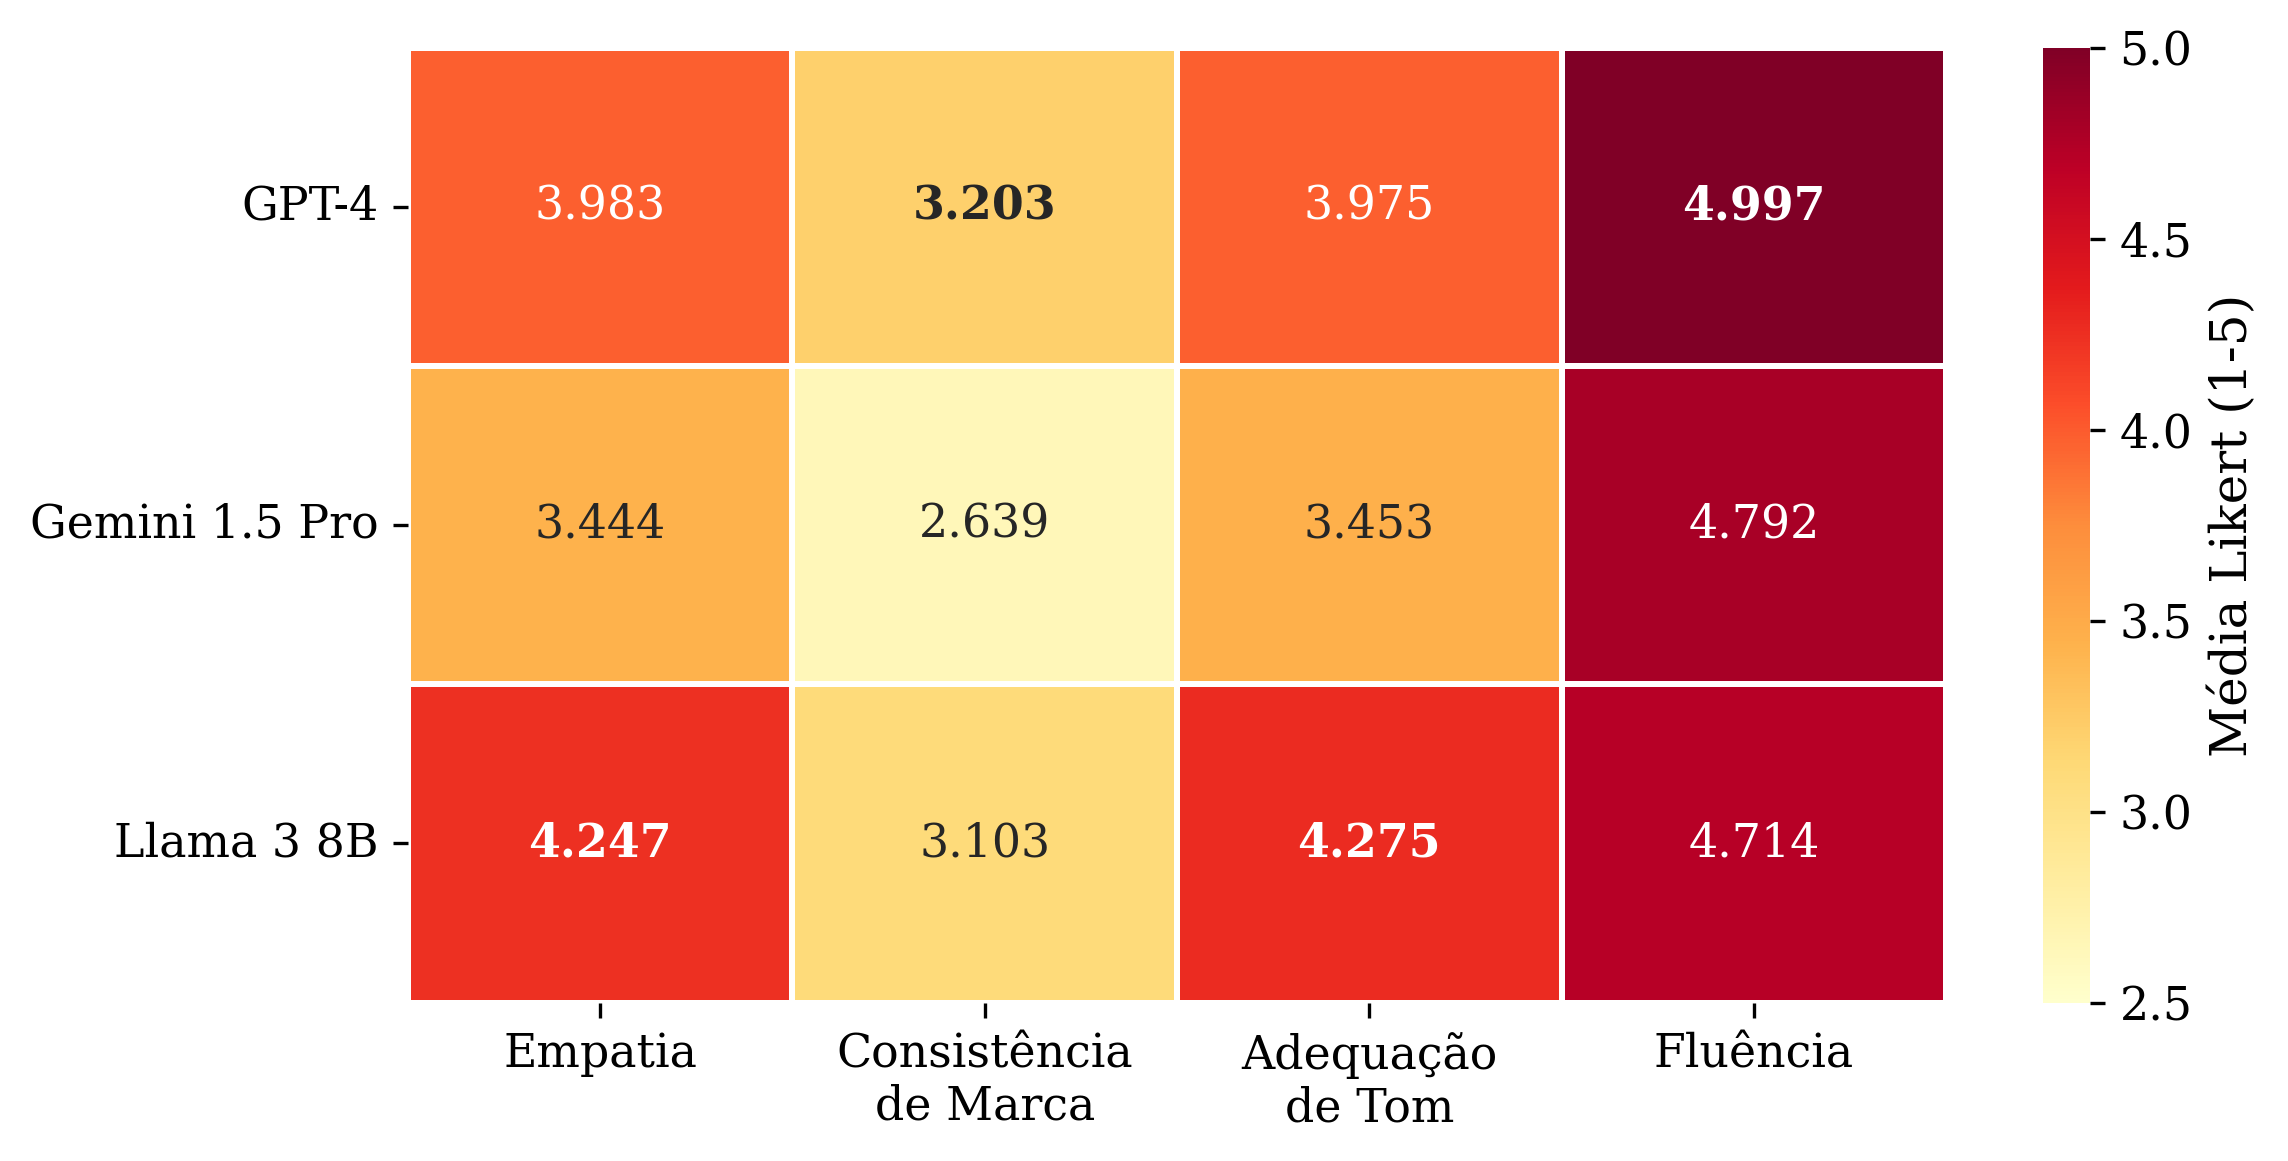
\includegraphics[width=0.85\textwidth]{img/heatmap_modelo_dimensao.png}
\caption{Mapa de calor das médias Likert por modelo e dimensão na avaliação humana.}
\label{fig:heatmap_modelo_dimensao}
\end{figure}

\subsection{Escolha dos testes estatísticos.}
 As variáveis-resposta deste estudo são pontuações em escala \textit{Likert} de 1 a 5 (variável 
ordinal discreta), provenientes de avaliações humanas e métricas automáticas que produzem 
distribuições assimétricas e tipicamente afastadas da normalidade. Em virtude da natureza ordinal 
dos dados e do não atendimento aos pressupostos paramétricos clássicos (normalidade e 
homogeneidade de variâncias), optou-se por testes não paramétricos baseados em \textit{ranks}. O 
teste de \textit{Kruskal-Wallis} foi adotado para verificar a existência de efeito global de 
modelo em cada dimensão, por se tratar da extensão não paramétrica da \textit{ANOVA} de um fator 
para mais de dois grupos independentes. Identificada significância, o teste de 
\textit{Mann-Whitney U} foi aplicado em comparações pareadas, por ser o equivalente não 
paramétrico do teste \textit{t} para amostras independentes. O nível de significância adotado foi 
$\alpha = 0{,}05$, com resultados de $p < 0{,}01$ considerados robustos e valores próximos ao 
limiar interpretados com cautela.

Para verificar se as diferenças entre modelos são estatisticamente significativas, aplicou-se o teste de \textit{Kruskal-Wallis} a cada dimensão. A Tabela~\ref{tab:kruskal} apresenta os resultados.

\begin{table}[H]
\centering
\caption{Teste de Kruskal-Wallis --- Efeito de Modelo na Avaliação Humana}
\label{tab:kruskal}
\begin{tabular}{@{}lccc@{}}
\toprule
\textbf{Dimensão} & \textbf{$H$} & \textbf{$p$-valor} & \textbf{Significativo ($\alpha = 0{,}05$)} \\ \midrule
Empatia & 6,44 & 0,040 & Sim \\
Consistência de marca & 8,14 & 0,017 & Sim \\
Adequação de tom & 10,66 & 0,005 & Sim ($p < 0{,}01$) \\
Fluência & 8,46 & 0,015 & Sim \\ \bottomrule
\end{tabular}
\end{table}

O efeito de modelo é estatisticamente significativo em todas as quatro dimensões ($p < 0{,}05$). Para identificar quais pares de modelos diferem entre si, realizaram-se comparações pareadas com o teste de \textit{Mann-Whitney U}. Os $p$-valores reportados na Tabela~\ref{tab:mannwhitney} são não corrigidos para comparações múltiplas; resultados com $p < 0{,}01$ são considerados robustos, enquanto aqueles próximos ao limiar de 0,05 devem ser interpretados com cautela.

\begin{table}[H]
\centering
\caption{Comparações Pareadas --- Teste de Mann-Whitney U ($p$-valores não corrigidos; cf.\ nota no texto)}
\label{tab:mannwhitney}
\resizebox{\textwidth}{!}{%
\begin{tabular}{@{}lccc@{}}
\toprule
\textbf{Dimensão} & \textbf{GPT-5.5 vs.\ Llama 4} & \textbf{GPT-5.5 vs.\ Gemini} & \textbf{Llama 4 vs.\ Gemini} \\ \midrule
Empatia & 0,391 (n.s.) & 0,097 (marginal) & \textbf{0,015} \\
Consistência de marca & 0,696 (n.s.) & \textbf{0,009} & \textbf{0,026} \\
Adequação de tom & 0,075 (marginal) & \textbf{0,046} & \textbf{0,003} \\
Fluência & \textbf{0,004} & \textbf{0,018} & 0,523 (n.s.) \\ \bottomrule
\end{tabular}%
}
\end{table}

As comparações pareadas revelam que a diferença estatisticamente mais robusta é a inferioridade do \textit{Gemini} em relação aos demais modelos: em empatia ($p = 0{,}015$ vs.\ \textit{Llama 4}), consistência de marca ($p = 0{,}009$ vs.\ \textit{GPT-5.5}; $p = 0{,}026$ vs.\ \textit{Llama 4}) e adequação de tom ($p = 0{,}003$ vs.\ \textit{Llama 4}; $p = 0{,}046$ vs.\ \textit{GPT-5.5}). Já \textit{GPT-5.5} e \textit{Llama 4} não diferem significativamente entre si em empatia ($p = 0{,}391$) e consistência de marca ($p = 0{,}696$), mas diferem em fluência ($p = 0{,}004$), onde o \textit{GPT-5.5} é superior.

A Figura~\ref{fig:boxplot_likert} apresenta a distribuição completa dos scores Likert por modelo e dimensão, permitindo a visualização da dispersão, medianas e \textit{outliers}.

\begin{figure}[H]
\centering
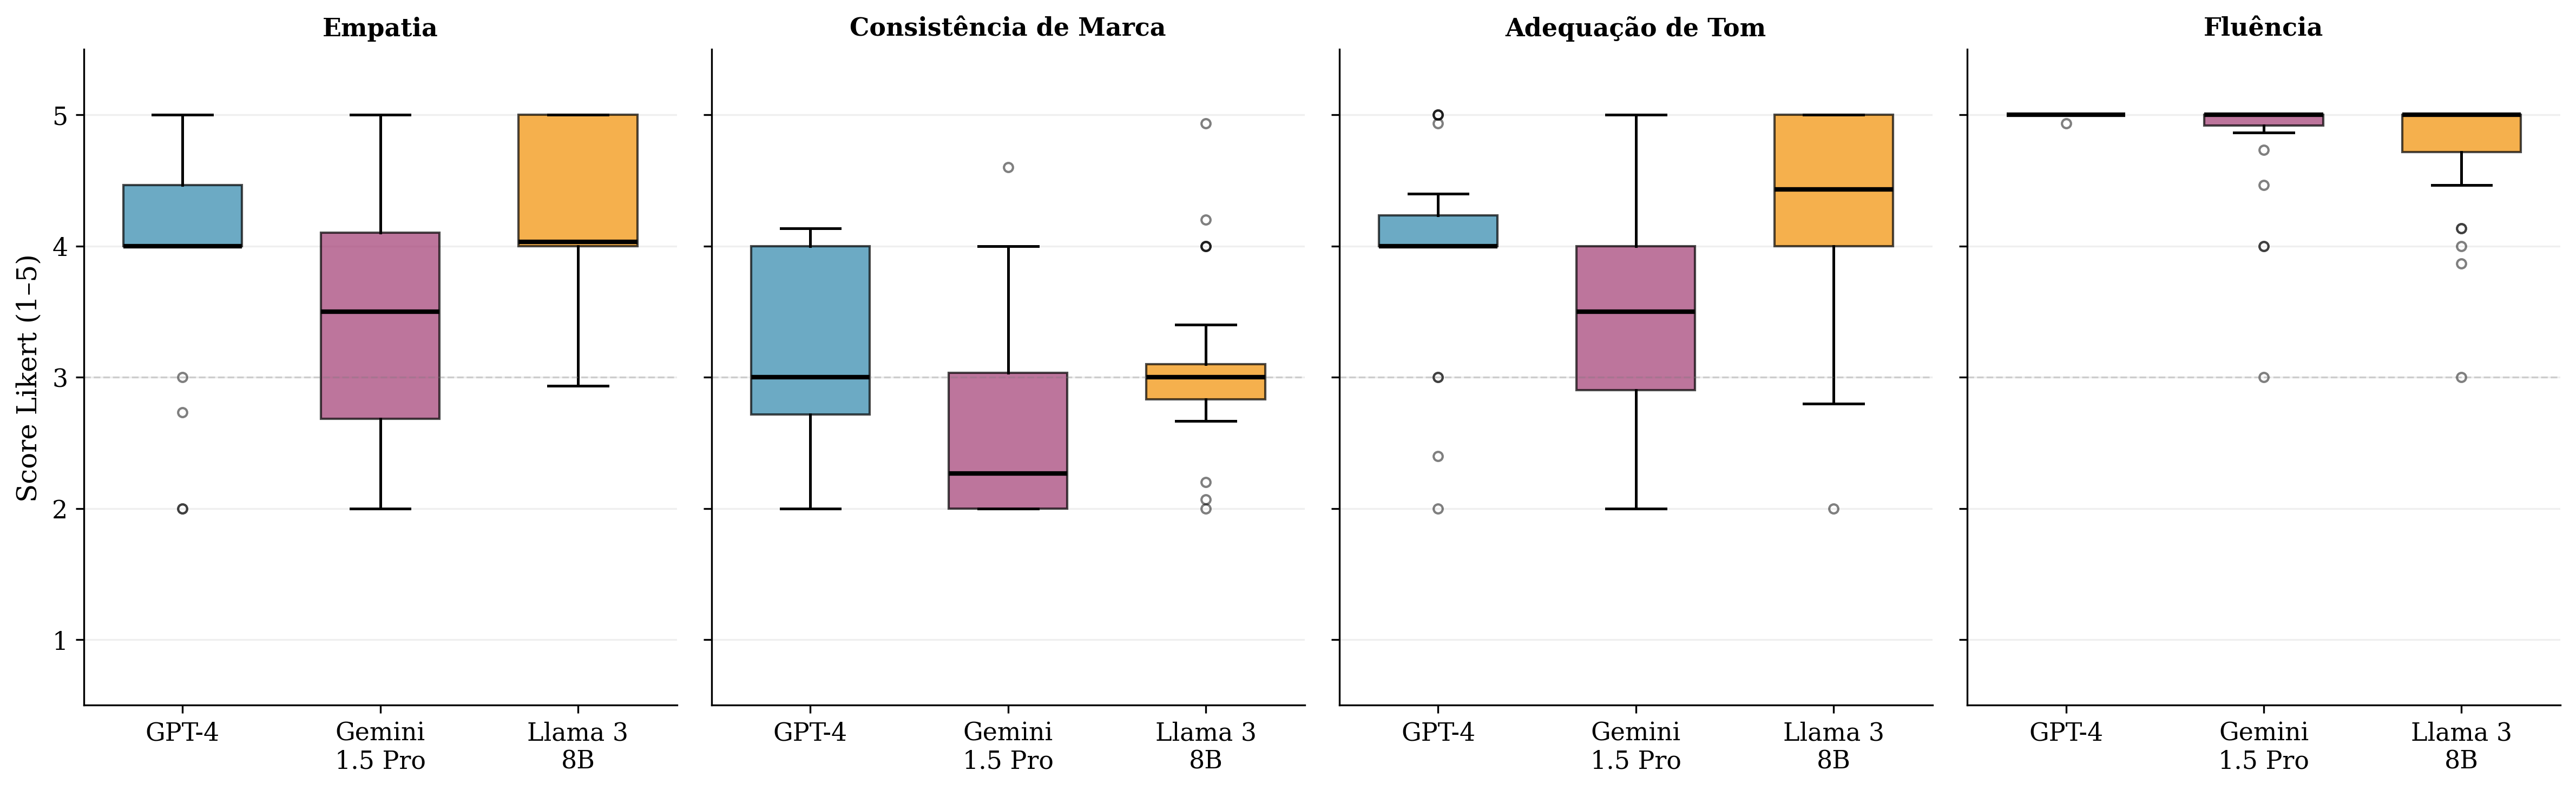
\includegraphics[width=\textwidth]{img/boxplot_likert.png}
\caption{Distribuição dos scores Likert por modelo e dimensão (média dos 15 avaliadores por item, $n = 72$ itens totais, $\approx$24 por modelo). \textit{Gemini} apresenta maior dispersão e medianas inferiores em empatia, consistência e tom. Fluência apresenta efeito teto para todos os modelos.}
\label{fig:boxplot_likert}
\end{figure}

\subsection{Métricas Automáticas}
\label{subsec:metricas_automaticas}

A Tabela~\ref{tab:auto_global} apresenta os resultados das quatro métricas automáticas utilizadas como \textit{proxies} computacionais para cada dimensão de qualidade.

\begin{table}[H]
\centering
\caption{Métricas Automáticas Globais por Modelo}
\label{tab:auto_global}
\resizebox{\textwidth}{!}{%
\begin{tabular}{@{}lcccc@{}}
\toprule
\textbf{Modelo} & \textbf{Empatia WASSA (1--5 $\uparrow$)} & \textbf{ToneCal TQS (0--1 $\uparrow$)} & \textbf{Fluência PPL ($\downarrow$)} & \textbf{Estilometria (0--1 $\uparrow$)} \\ \midrule
\textit{GPT-5.5} & \textbf{3,360} & 0,544 & \textbf{118,3} & 0,061 \\
\textit{Llama 4} & 3,280 & \textbf{0,582} & 229,4 & 0,052 \\
\textit{Gemini 3.1} & 3,113 & 0,513 & 179,5 & \textbf{0,070} \\ \bottomrule
\end{tabular}%
}
\end{table}

Na dimensão de fluência (perplexidade GPT-2), o \textit{GPT-5.5} apresenta a menor perplexidade média (118,3), indicando maior fluência textual, seguido pelo \textit{Gemini} (179,5) e \textit{Llama 4} (229,4). No ToneCal (adequação de tom), o \textit{Llama 4} lidera com TQS médio de 0,582, seguido pelo \textit{GPT-5.5} (0,544) e \textit{Gemini} (0,513). Na empatia percebida (WASSA), o \textit{GPT-5.5} obtém o maior escore (3,360), seguido pelo \textit{Llama 4} (3,280) e \textit{Gemini} (3,113), nota-se que, diferentemente da avaliação humana, a métrica WASSA posiciona o \textit{GPT-5.5} em primeiro lugar. Na similaridade estilométrica (\textit{Writeprints}), o \textit{Gemini} apresenta o maior valor (0,070), seguido pelo \textit{GPT-5.5} (0,061) e \textit{Llama 4} (0,052). Os valores absolutos de similaridade estilométrica são uniformemente baixos ($< 0{,}08$), refletindo a diferença inerente entre texto gerado por \textit{LLMs} e texto humano; a utilidade principal da métrica reside na comparação relativa entre modelos.

Esses resultados corroboram parcialmente a avaliação humana: os rankings de fluência e adequação de tom convergem entre as duas modalidades, enquanto os de empatia e consistência de marca divergem. As divergências são analisadas em detalhe na Seção~\ref{subsec:convergencias}.

A Figura~\ref{fig:barras_comparativas} apresenta uma comparação visual lado a lado entre avaliação humana e métricas automáticas.

\begin{figure}[H]
\centering
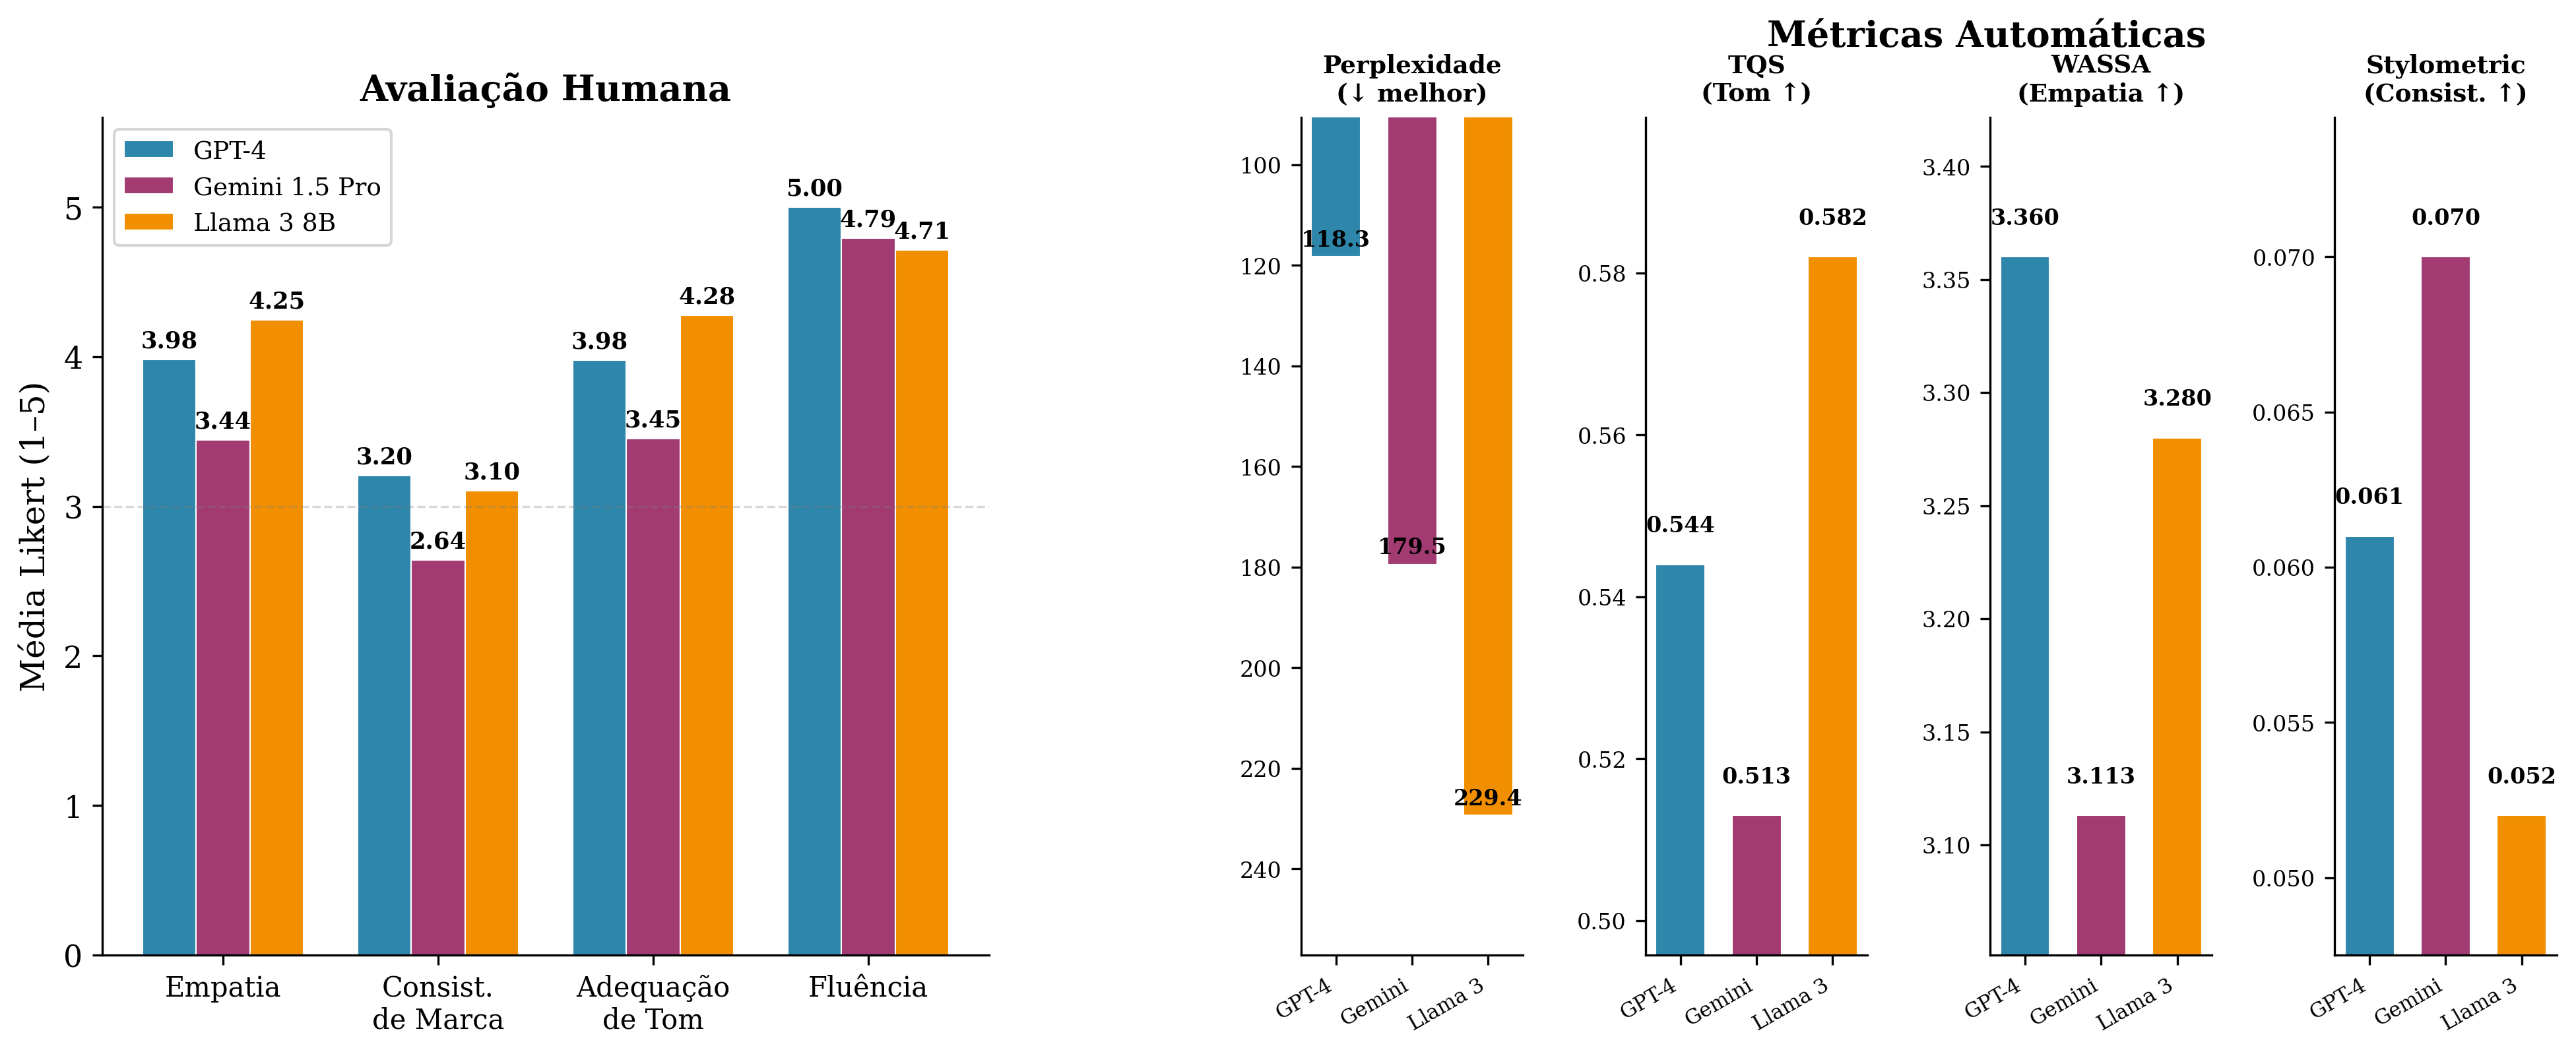
\includegraphics[width=\textwidth]{img/barras_comparativas_modelos.png}
\caption{Comparação entre os três modelos nas avaliações humana (esquerda, escala Likert 1--5) e automática (direita, escalas individuais por métrica).}
\label{fig:barras_comparativas}
\end{figure}

A Figura~\ref{fig:radar_multidimensional} sintetiza o perfil multidimensional de cada modelo, integrando as oito métricas (quatro humanas e quatro automáticas) em uma representação normalizada.

\begin{figure}[H]
\centering
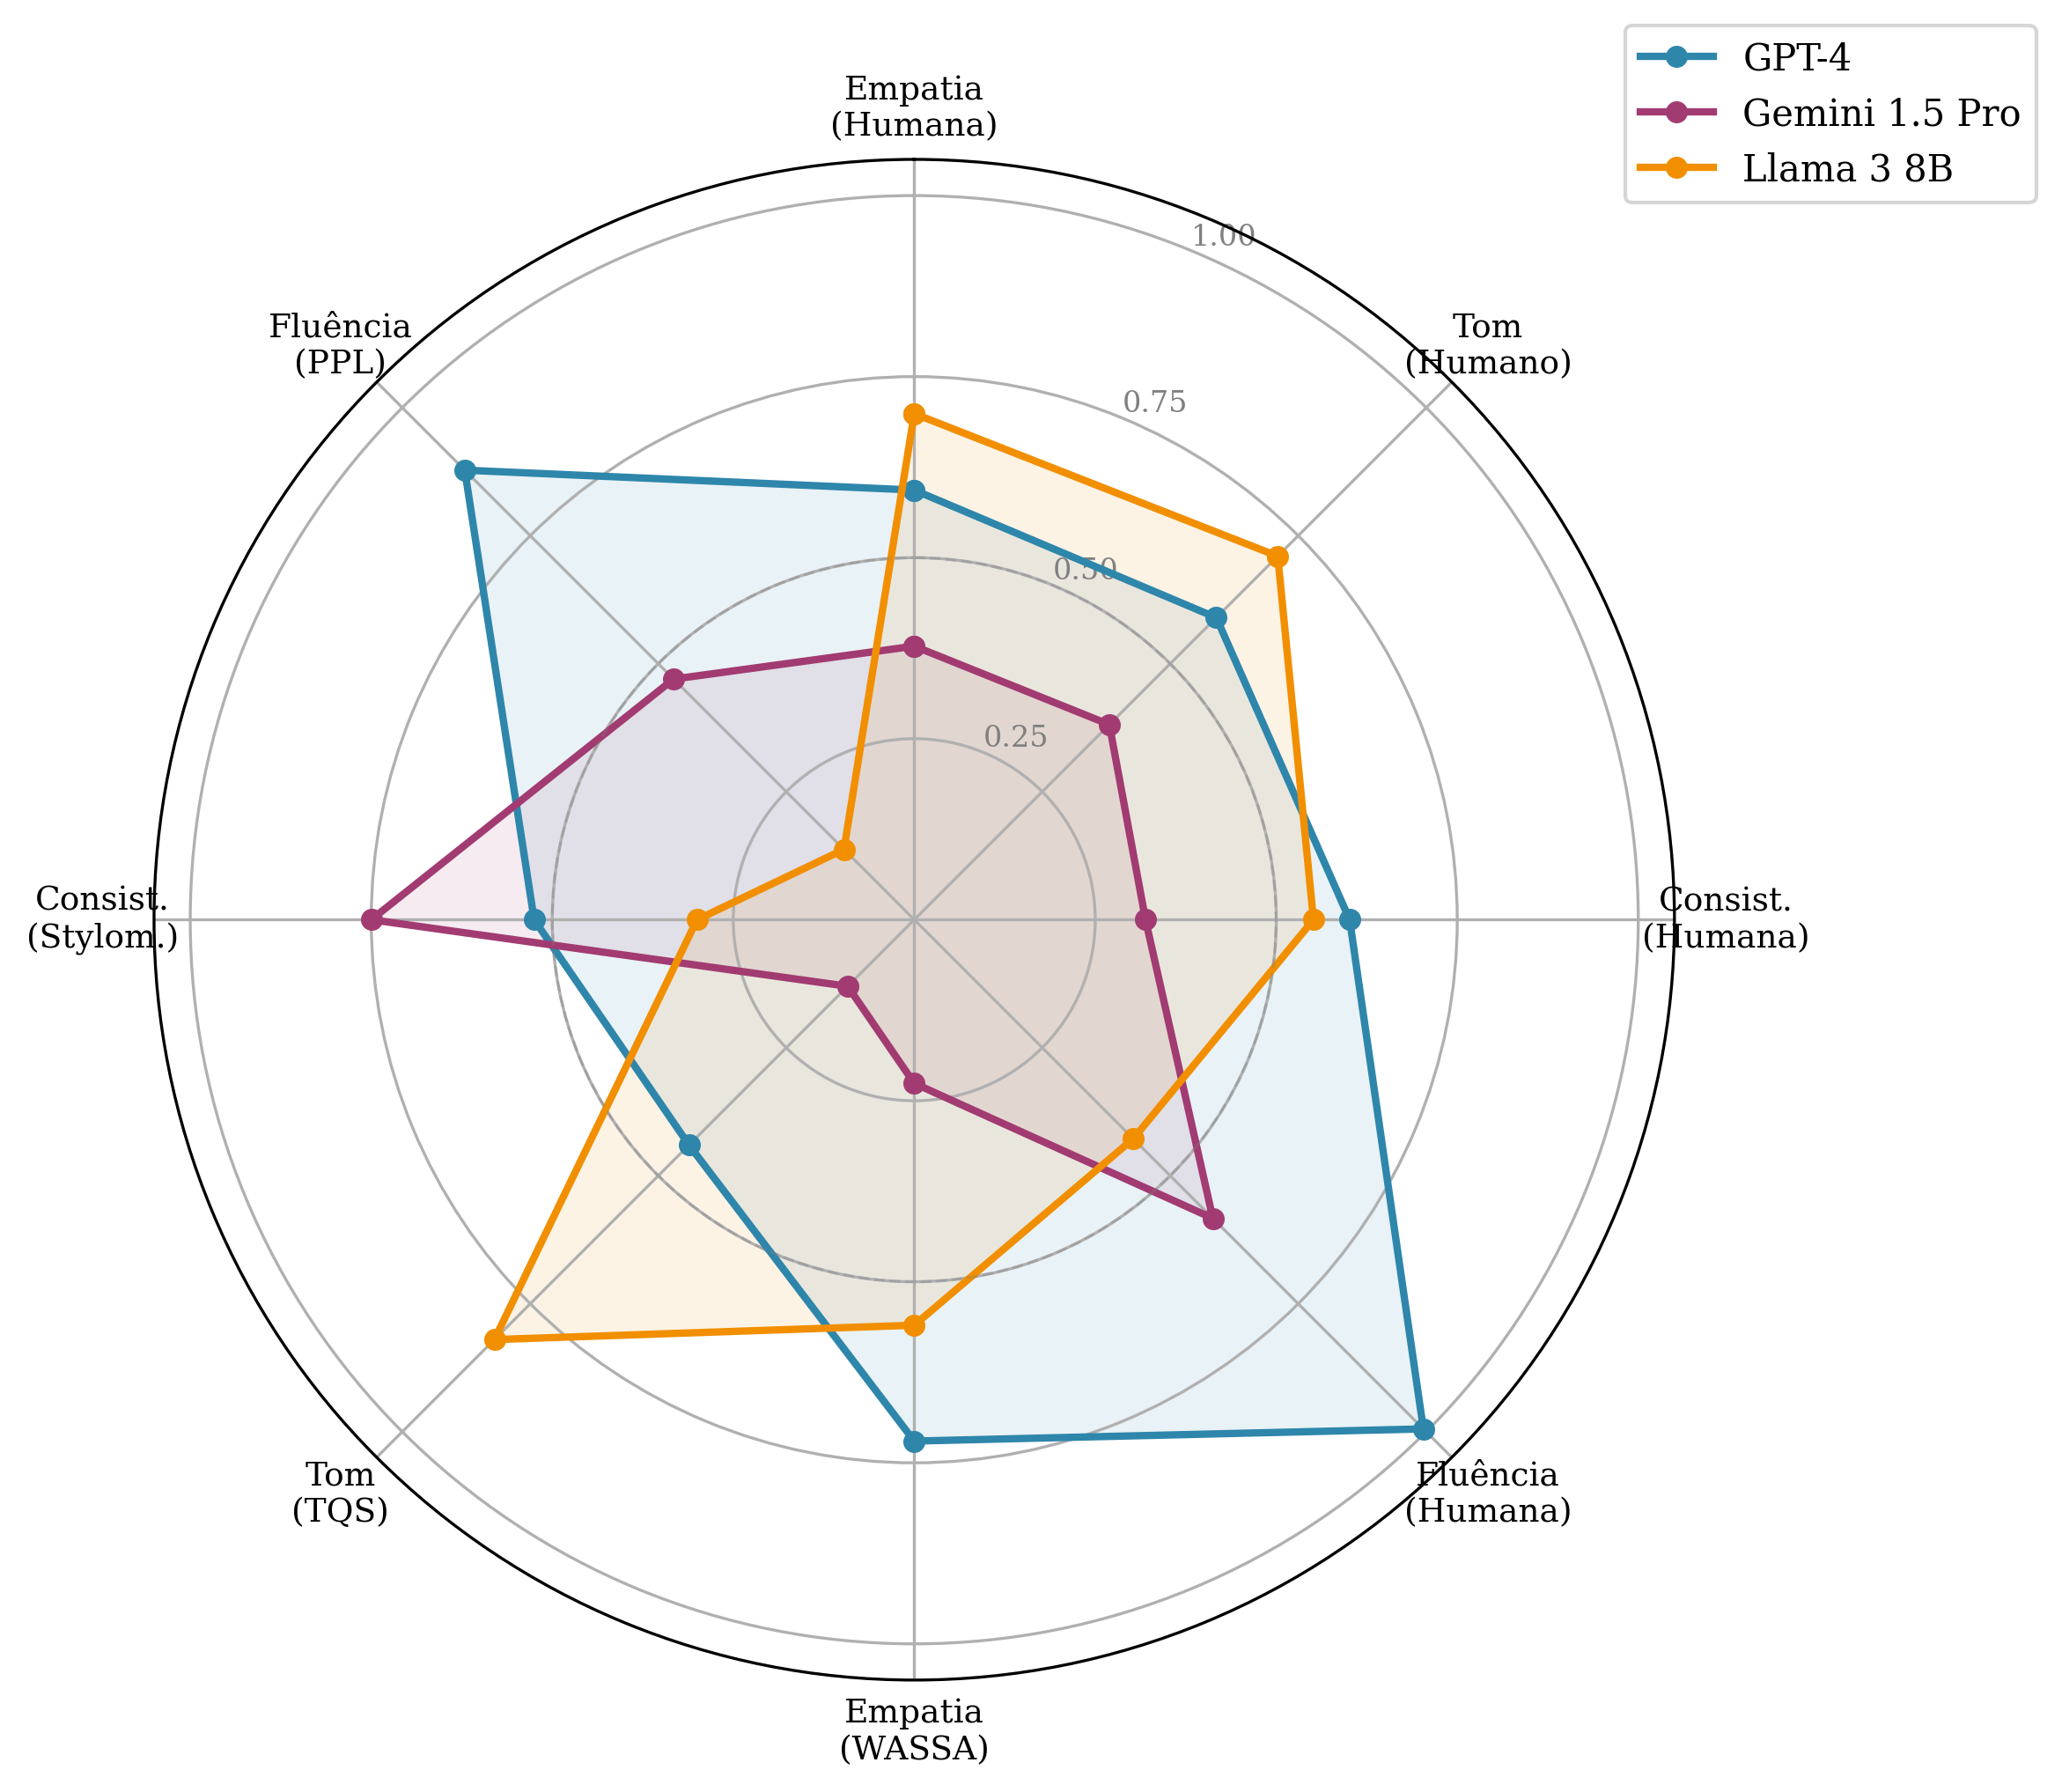
\includegraphics[width=0.75\textwidth]{img/radar_multidimensional.png}
\caption{Perfil multidimensional dos modelos combinando métricas humanas e automáticas (valores normalizados 0--1).}
\label{fig:radar_multidimensional}
\end{figure}

\subsection{Análise Estratificada}
\label{subsec:estratificada}

\subsubsection{Interação Modelo $\times$ Persona}

A Tabela~\ref{tab:modelo_persona} apresenta a avaliação humana estratificada por modelo e persona.

\begin{table}[H]
\centering
\caption{Avaliação Humana por Modelo e Persona (escala Likert 1--5)}
\label{tab:modelo_persona}
\resizebox{\textwidth}{!}{%
\begin{tabular}{@{}llcccc@{}}
\toprule
\textbf{Modelo} & \textbf{Persona} & \textbf{Empatia} & \textbf{Consist. Marca} & \textbf{Adeq. Tom} & \textbf{Fluência} \\ \midrule
\textit{Llama 4} & P2 (informal) & \textbf{4,306} & 3,044 & \textbf{4,289} & 4,511 \\
\textit{Llama 4} & P1 (formal) & 4,189 & 3,161 & 4,261 & 4,917 \\
\textit{GPT-5.5} & P2 (informal) & 4,039 & \textbf{3,378} & 4,039 & \textbf{5,000} \\
\textit{GPT-5.5} & P1 (formal) & 3,928 & 3,028 & 3,911 & 4,994 \\
\textit{Gemini 3.1} & P2 (informal) & 3,606 & 2,706 & 3,667 & 4,667 \\
\textit{Gemini 3.1} & P1 (formal) & 3,283 & 2,572 & 3,239 & 4,917 \\ \bottomrule
\end{tabular}%
}
\end{table}

Na avaliação humana, a persona informal (P2, acolhedora) recebe pontuações superiores em empatia, consistência de marca e adequação de tom para \textit{todos} os modelos. Em contrapartida, as métricas automáticas (WASSA: P1 $= 3{,}329$ vs.\ P2 $= 3{,}205$; ToneCal: P1 $= 0{,}555$ vs.\ P2 $= 0{,}538$) favorecem sistematicamente a persona formal (P1, sofisticada). Essa inversão direcional, discutida na Seção~\ref{subsec:convergencias}, constitui evidência de viés compartilhado dos \textit{proxies} automáticos para registro formal. A persona formal é superior apenas em fluência, dimensão na qual avaliação humana e métricas automáticas convergem.

A sensibilidade ao efeito de persona varia entre modelos. O \textit{Gemini} apresenta a maior sensibilidade: a diferença entre P2 e P1 em adequação de tom atinge $+0{,}428$ pontos e em empatia $+0{,}322$ pontos. No \textit{Llama 4}, essas diferenças são menores ($+0{,}028$ em tom e $+0{,}117$ em empatia), indicando que seu desempenho é mais estável entre personas.

\subsubsection{Interação Modelo $\times$ Estratégia de \textit{Prompt}}

A Tabela~\ref{tab:modelo_prompt} estratifica os resultados humanos por modelo e estratégia de \textit{prompt}.

\begin{table}[H]
\centering
\caption{Avaliação Humana por Modelo e Estratégia de \textit{Prompt} (escala Likert 1--5)}
\label{tab:modelo_prompt}
\resizebox{\textwidth}{!}{%
\begin{tabular}{@{}llcccc@{}}
\toprule
\textbf{Modelo} & \textbf{Estratégia} & \textbf{Empatia} & \textbf{Consist. Marca} & \textbf{Adeq. Tom} & \textbf{Fluência} \\ \midrule
\textit{Llama 4} & \textit{zero-shot} & \textbf{4,339} & 3,128 & \textbf{4,367} & 4,611 \\
\textit{Llama 4} & \textit{few-shot} & 4,156 & 3,078 & 4,183 & 4,817 \\
\textit{GPT-5.5} & \textit{zero-shot} & 4,100 & 3,128 & 4,111 & 4,994 \\
\textit{GPT-5.5} & \textit{few-shot} & 3,867 & \textbf{3,278} & 3,839 & \textbf{5,000} \\
\textit{Gemini 3.1} & \textit{zero-shot} & 3,772 & 2,656 & 3,806 & 4,944 \\
\textit{Gemini 3.1} & \textit{few-shot} & 3,117 & 2,622 & 3,100 & 4,639 \\ \bottomrule
\end{tabular}%
}
\end{table}

Na avaliação humana, a estratégia \textit{zero-shot} tende a superar a \textit{few-shot} em empatia ($\Delta = +0{,}357$, $p = 0{,}074$, marginalmente significativo) e adequação de tom ($\Delta = +0{,}387$) para \textit{todos} os modelos, com magnitudes que variam conforme o modelo. Embora o efeito global de estratégia não atinja significância estatística ao nível convencional de 5\%, a consistência direcional em todos os modelos reforça a tendência observada. O efeito é particularmente acentuado no \textit{Gemini}, onde o \textit{zero-shot} supera o \textit{few-shot} em $+0{,}655$ pontos de empatia e $+0{,}706$ pontos de adequação de tom. Para o \textit{GPT-5.5}, as diferenças são de $+0{,}233$ (empatia) e $+0{,}272$ (tom); para o \textit{Llama 4}, de $+0{,}183$ em ambas as dimensões.

Esse padrão sugere que exemplos \textit{few-shot} podem restringir a expressividade dos modelos, gerando respostas mais templáticas que os avaliadores humanos percebem como menos empáticas e menos adequadas ao tom. A estratégia \textit{few-shot} apresenta vantagem apenas em consistência de marca para o \textit{GPT-5.5} ($+0{,}150$) e em fluência para o \textit{Llama 4} ($+0{,}206$). As métricas automáticas, por outro lado, não detectam a superioridade do \textit{zero-shot}: a diferença em empatia WASSA entre as duas estratégias é de apenas $\Delta = 0{,}003$ ($\textit{few-shot} = 3{,}253$; $\textit{zero-shot} = 3{,}250$), sugerindo que os avaliadores humanos são sensíveis a nuances de expressividade que os \textit{proxies} computacionais não capturam.

\subsubsection{Interação Modelo $\times$ Período Temporal}

A Tabela~\ref{tab:modelo_periodo} apresenta os resultados estratificados por modelo e período temporal.

\begin{table}[H]
\centering
\caption{Avaliação Humana por Modelo e Período (escala Likert 1--5)}
\label{tab:modelo_periodo}
\resizebox{\textwidth}{!}{%
\begin{tabular}{@{}llcccc@{}}
\toprule
\textbf{Modelo} & \textbf{Período} & \textbf{Empatia} & \textbf{Consist. Marca} & \textbf{Adeq. Tom} & \textbf{Fluência} \\ \midrule
\textit{Llama 4} & \textit{after} & \textbf{4,489} & 3,200 & \textbf{4,561} & 4,633 \\
\textit{GPT-5.5} & \textit{after} & 4,061 & 3,222 & 4,156 & 4,994 \\
\textit{Llama 4} & \textit{before} & 4,006 & 3,006 & 3,989 & 4,794 \\
\textit{GPT-5.5} & \textit{before} & 3,906 & 3,183 & 3,794 & \textbf{5,000} \\
\textit{Gemini 3.1} & \textit{after} & 3,589 & 2,450 & 3,600 & 4,978 \\
\textit{Gemini 3.1} & \textit{before} & 3,300 & 2,828 & 3,306 & 4,606 \\ \bottomrule
\end{tabular}%
}
\end{table}

O período \textit{after} (após a popularização das LLMs) está associado a maiores pontuações de empatia ($\Delta = +0{,}309$, $p = 0{,}029$) e adequação de tom ($\Delta = +0{,}409$, $p = 0{,}019$) na avaliação humana. O \textit{Llama 4} apresenta o maior benefício do período \textit{after} ($\Delta = +0{,}483$ em empatia e $+0{,}572$ em tom), enquanto o \textit{GPT-5.5} é o modelo menos sensível ao período ($\Delta = +0{,}156$ em empatia). O \textit{Gemini} apresenta uma anomalia na dimensão de consistência de marca: obtém resultado superior no período \textit{before} (2,828) em comparação com o \textit{after} (2,450), contrariando a tendência geral dos demais modelos.

Cabe notar que os comentários-base diferem entre os dois períodos (100 distintos em cada), de modo que os resultados desta subseção representam tendências descritivas associadas ao período, e não efeitos causais isolados.

\subsubsection{Melhores e Piores Cenários}

A Tabela~\ref{tab:top_bottom_cenarios} apresenta os cinco cenários com maiores e menores médias de empatia na avaliação humana, permitindo identificar as combinações experimentais ótimas e subótimas.

\begin{table}[H]
\centering
\caption{Top 5 e Bottom 5 Cenários por Empatia na Avaliação Humana}
\label{tab:top_bottom_cenarios}
\resizebox{\textwidth}{!}{%
\begin{tabular}{@{}clcccc@{}}
\toprule
\textbf{Rank} & \textbf{Cenário} & \textbf{Empatia} & \textbf{Adeq.\ Tom} & \textbf{Consist.\ Marca} & \textbf{Fluência} \\ \midrule
\multicolumn{6}{l}{\textit{Top 5}} \\
1 & Llama 4 --- P1, \textit{few-shot}, \textit{after} & \textbf{4,644} & 4,622 & \textbf{3,733} & 5,000 \\
2 & Llama 4 --- P2, \textit{few-shot}, \textit{after} & 4,600 & \textbf{4,822} & 3,333 & 4,711 \\
3 & Gemini --- P2, \textit{zero-shot}, \textit{before} & 4,600 & 4,667 & 3,222 & 5,000 \\
4 & GPT-5.5 --- P1, \textit{few-shot}, \textit{after} & 4,489 & 4,400 & 3,244 & 5,000 \\
5 & GPT-5.5 --- P2, \textit{zero-shot}, \textit{after} & 4,422 & 4,333 & 3,022 & 5,000 \\ \midrule
\multicolumn{6}{l}{\textit{Bottom 5}} \\
20 & Gemini --- P2, \textit{few-shot}, \textit{after} & 3,333 & 3,333 & 2,711 & 5,000 \\
21 & GPT-5.5 --- P1, \textit{few-shot}, \textit{before} & 3,267 & 3,133 & 2,533 & 5,000 \\
22 & Gemini --- P1, \textit{few-shot}, \textit{after} & 3,111 & 3,044 & 2,067 & 4,911 \\
23 & Gemini --- P2, \textit{few-shot}, \textit{before} & 2,667 & 2,689 & 2,400 & 3,667 \\
24 & Gemini --- P1, \textit{zero-shot}, \textit{before} & 2,578 & 2,533 & 2,378 & 4,778 \\ \bottomrule
\end{tabular}%
}
\end{table}

Os melhores cenários concentram-se no período \textit{after} (4 dos 5 primeiros), com \textit{Llama 4} e \textit{GPT-5.5} ocupando a maioria das posições de destaque. Os piores cenários são dominados pelo \textit{Gemini}, que ocupa 4 das 5 últimas posições, predominantemente com a estratégia \textit{few-shot}. Notavelmente, o \textit{Gemini} com persona informal e \textit{zero-shot} no período \textit{before} atinge empatia de 4,600 (2º lugar), demonstrando que, sob condições específicas, até o modelo de pior desempenho global pode atingir resultados competitivos.

\subsection{Análise Qualitativa: Exemplos Ilustrativos}
 \label{subsec:analise_qualitativa}
 
 Para complementar a análise quantitativa apresentada nas seções anteriores e oferecer uma 
compreensão concreta dos padrões observados, esta seção apresenta exemplos representativos 
extraídos do \textit{Corpus Resultante}. Os trechos foram selecionados de forma a ilustrar 
diferentes cenários identificados na análise estratificada, com ênfase na justaposição entre 
comentário original e resposta gerada.
 
 \subsubsection*{Exemplo 1: Resposta bem avaliada (alta empatia e adequação ao contexto)}
 
 \noindent\textbf{Comentário do cliente:}
 \begin{quote}
 \textit{``Tenho carinho pelo restaurante, mas nesta visita saí com sensação mista. Fomos no 
comemoração de namoro e pedimos camarão Iracema. O prato estava bom, embora eu esperasse mais pelo
 valor cobrado. A climatização boa ajuda bastante, mas o prato veio morno e isso comprometeu a 
experiência.''}
 \end{quote}
 
 \noindent\textbf{Resposta gerada (\textit{Llama 4}, persona formal, \textit{zero-shot}):}
 \begin{quote}
 \textit{``Muito obrigado por compartilhar sua experiência conosco. Ficamos felizes que parte da 
experiência foi positiva, mas lamentamos que o prato tenha chegado morno e comprometido o momento 
da comemoração. Estamos sempre trabalhando para melhorar e esperamos recebê-lo novamente em uma 
próxima oportunidade.''}
 \end{quote}
 
 \noindent\textit{Análise:} a resposta reconhece explicitamente os dois polos do comentário 
(positivo e negativo), referencia o aspecto específico mencionado (prato morno), contextualiza o 
evento (comemoração) e encerra com uma expectativa concreta de retorno. Esse padrão de 
\textit{acknowledgement balanceado} é característico das respostas com pontuações humanas elevadas
 em empatia e adequação de tom.
 
 \subsubsection*{Exemplo 2: Resposta fluente, mas pouco empática}
 
 \noindent\textbf{Comentário do cliente:}
 \begin{quote}
 \textit{``Tivemos uma ótima experiência no aniversário. Pedimos bolinho de bacalhau e feijão 
baião, ambos bem servidos e saborosos. A decoração sofisticada fez diferença e o atendimento do 
Lucas foi atencioso do início ao fim.''}
 \end{quote}
 
 \noindent\textbf{Resposta gerada (\textit{Gemini 3.1}, persona formal, \textit{zero-shot}):}
 \begin{quote}
 \textit{``É com satisfação que recebemos seu elogio ao nosso ambiente e ao serviço prestado. 
Nosso compromisso é oferecer uma atmosfera acolhedora aliada a um padrão gastronômico de elite, 
garantindo experiências únicas a cada visita.''}
 \end{quote}
 
 \noindent\textit{Análise:} embora a resposta seja gramaticalmente correta e fluente, ela ignora 
os elementos específicos mencionados pelo cliente: o aniversário, o nome do atendente (Lucas) e os
 pratos referenciados. A construção é genérica e poderia ser aplicada a qualquer comentário 
positivo, configurando o padrão \textit{templático} associado a baixas pontuações humanas de 
empatia, ainda que com fluência elevada nas métricas automáticas.
 
 \subsubsection*{Exemplo 3: Resposta excessivamente formal}
 
 \noindent\textbf{Comentário do cliente:}
 \begin{quote}
 \textit{``Ambiente agradável e experiência muito positiva no happy hour. Pedimos lagosta grelhada
 e arroz dos mares, ambos bem servidos e saborosos. A música ao vivo agradável fez diferença e o 
atendimento do Wellington foi atencioso do início ao fim.''}
 \end{quote}
 
 \noindent\textbf{Resposta gerada (\textit{GPT-5.5}, persona formal, \textit{few-shot}):}
 \begin{quote}
 \textit{``Ficamos honrados com seu registro e com a generosidade de sua avaliação. É 
especialmente gratificante saber que sua experiência no happy hour foi marcada de forma tão 
positiva. Será uma satisfação compartilhar seu reconhecimento ao atendimento de Wellington com a 
equipe.''}
 \end{quote}
 
 \noindent\textit{Análise:} a resposta utiliza um registro elevado, ``honrados'', 
``generosidade de sua avaliação'', ``especialmente gratificante'' que, em um contexto de 
\textit{review} público de restaurante, foi consistentemente percebido pelos avaliadores humanos como rebuscado e distante. Esse tipo de construção é favorecido pelas métricas automáticas (perplexidade e \textit{ToneCal}) por sua aderência ao registro formal, mas penalizado na avaliação humana por reduzir a sensação de proximidade e acolhimento.
 
 \subsubsection*{Exemplo 4: Resposta inconsistente com o contexto do comentário}
 
 \noindent\textbf{Comentário do cliente:}
 \begin{quote}
 \textit{``A proposta do restaurante é boa, mas o serviço não acompanhou. Fomos no comemoração de namoro e enfrentamos música muito alta logo no início. Quando o moqueca de camarão chegou, veio com aspecto abaixo do esperado e o prato estava morno. Houve ainda tempo de espera acima do esperado, o que comprometeu a noite.''}
 \end{quote}
 
 \noindent\textbf{Resposta gerada (\textit{GPT-5.5}, persona formal, \textit{zero-shot}):}
 \begin{quote}
 \textit{``É uma alegria saber que sua experiência foi tão positiva. Nossa proposta gastronômica é cuidadosamente pensada para proporcionar uma experiência marcante. Compreendemos que o tempo de espera impacta diretamente a experiência e levamos essa observação em consideração.''}
 \end{quote}
 
 \noindent\textit{Análise:} este caso ilustra uma falha de leitura do sentimento do comentário: o cliente relata uma experiência majoritariamente negativa (música alta, prato morno, demora), mas a resposta abre com uma afirmação de comemoração (``É uma alegria saber que sua experiência foi tão positiva''), claramente desalinhada com o conteúdo recebido. Apesar de gramaticalmente correta e estilisticamente coerente com a persona formal, a resposta evidencia o que \citeonline{liang2023} caracterizam como \textit{descolamento pragmático}: aderência à forma sem aderência ao significado.
 
 \subsubsection*{Exemplo 5: Comparação Zero-Shot vs.\ Few-Shot para o mesmo comentário}
 
 \noindent\textbf{Comentário do cliente:}
 \begin{quote}
 \textit{``Tenho carinho pelo restaurante, mas nesta visita saí com sensação mista. [...] o prato 
veio morno e isso comprometeu a experiência.''}
 \end{quote}
 
 \noindent\textbf{Resposta \textit{Zero-Shot} (\textit{Llama 4}, persona formal):}
 \begin{quote}
 \textit{``Muito obrigado por compartilhar sua experiência conosco. Ficamos felizes que parte da 
experiência foi positiva, mas lamentamos que o prato tenha chegado morno e comprometido o momento 
da comemoração. Estamos sempre trabalhando para melhorar e esperamos recebê-lo novamente.''}
 \end{quote}
 
 \noindent\textbf{Resposta \textit{Few-Shot} (\textit{Llama 4}, persona formal):}
 \begin{quote}
 \textit{``Prezado(a) cliente, agradecemos por compartilhar sua experiência. Ficamos satisfeitos 
que parte da experiência tenha sido agradável, e lamentamos pelo prato veio morno. Esperamos 
recebê-lo(a) novamente.''}
 \end{quote}
 
 \noindent\textit{Análise:} a comparação direta entre as duas estratégias para o mesmo comentário 
ilustra o padrão quantitativo identificado na Seção~\ref{subsec:estratificada}: a resposta 
\textit{zero-shot} é mais extensa, contextualiza o evento (``comemoração''), inclui um compromisso
 (``estamos sempre trabalhando para melhorar'') e evita fórmulas de tratamento rígidas. A resposta
 \textit{few-shot}, em contraste, adota a estrutura dos exemplos demonstrativos, abertura com ``Prezado(a) cliente'', construções mais formulaicas e encerramento curto, evidenciando como exemplos podem reduzir a expressividade do modelo. Este padrão, observado de forma consistente nos três modelos avaliados, fundamenta a recomendação operacional pela abordagem \textit{zero-shot} com persona bem definida (Seção~\ref{subsec:implicacoes}).

\subsection{Convergências e Divergências entre Avaliação Humana e Automática}

A triangulação entre avaliação humana e métricas automáticas constitui um dos achados metodológicos centrais deste estudo. A Tabela~\ref{tab:convergencia} sintetiza a comparação dos rankings por dimensão, enquanto a Figura~\ref{fig:dispersao_humano_automatico} apresenta a dispersão entre as duas modalidades de avaliação, estratificada por modelo e persona.


\begin{table}[H]
\centering
\caption{Convergência de Rankings: Avaliação Humana vs.\ Métricas Automáticas}
\label{tab:convergencia}
\resizebox{\textwidth}{!}{%
\begin{tabular}{@{}llll@{}}
\toprule
\textbf{Dimensão} & \textbf{Ranking Humano} & \textbf{Ranking Automático} & \textbf{Convergência} \\ \midrule
Adequação de tom & Llama 4 $>$ GPT-5.5 $>$ Gemini & Llama 4 $>$ GPT-5.5 $>$ Gemini (TQS) & Forte \\
Fluência & GPT-5.5 $>$ Gemini $>$ Llama 4 & GPT-5.5 $>$ Gemini $>$ Llama 4 (PPL) & Forte \\
Empatia & Llama 4 $>$ GPT-5.5 $>$ Gemini & GPT-5.5 $>$ Llama 4 $>$ Gemini (WASSA) & Parcial \\
Consist. de marca & GPT-5.5 $>$ Llama 4 $>$ Gemini & Gemini $>$ GPT-5.5 $>$ Llama 4 (Estil.) & Divergente \\ \bottomrule
\end{tabular}%
}
\end{table}


\begin{figure}[H]
\centering
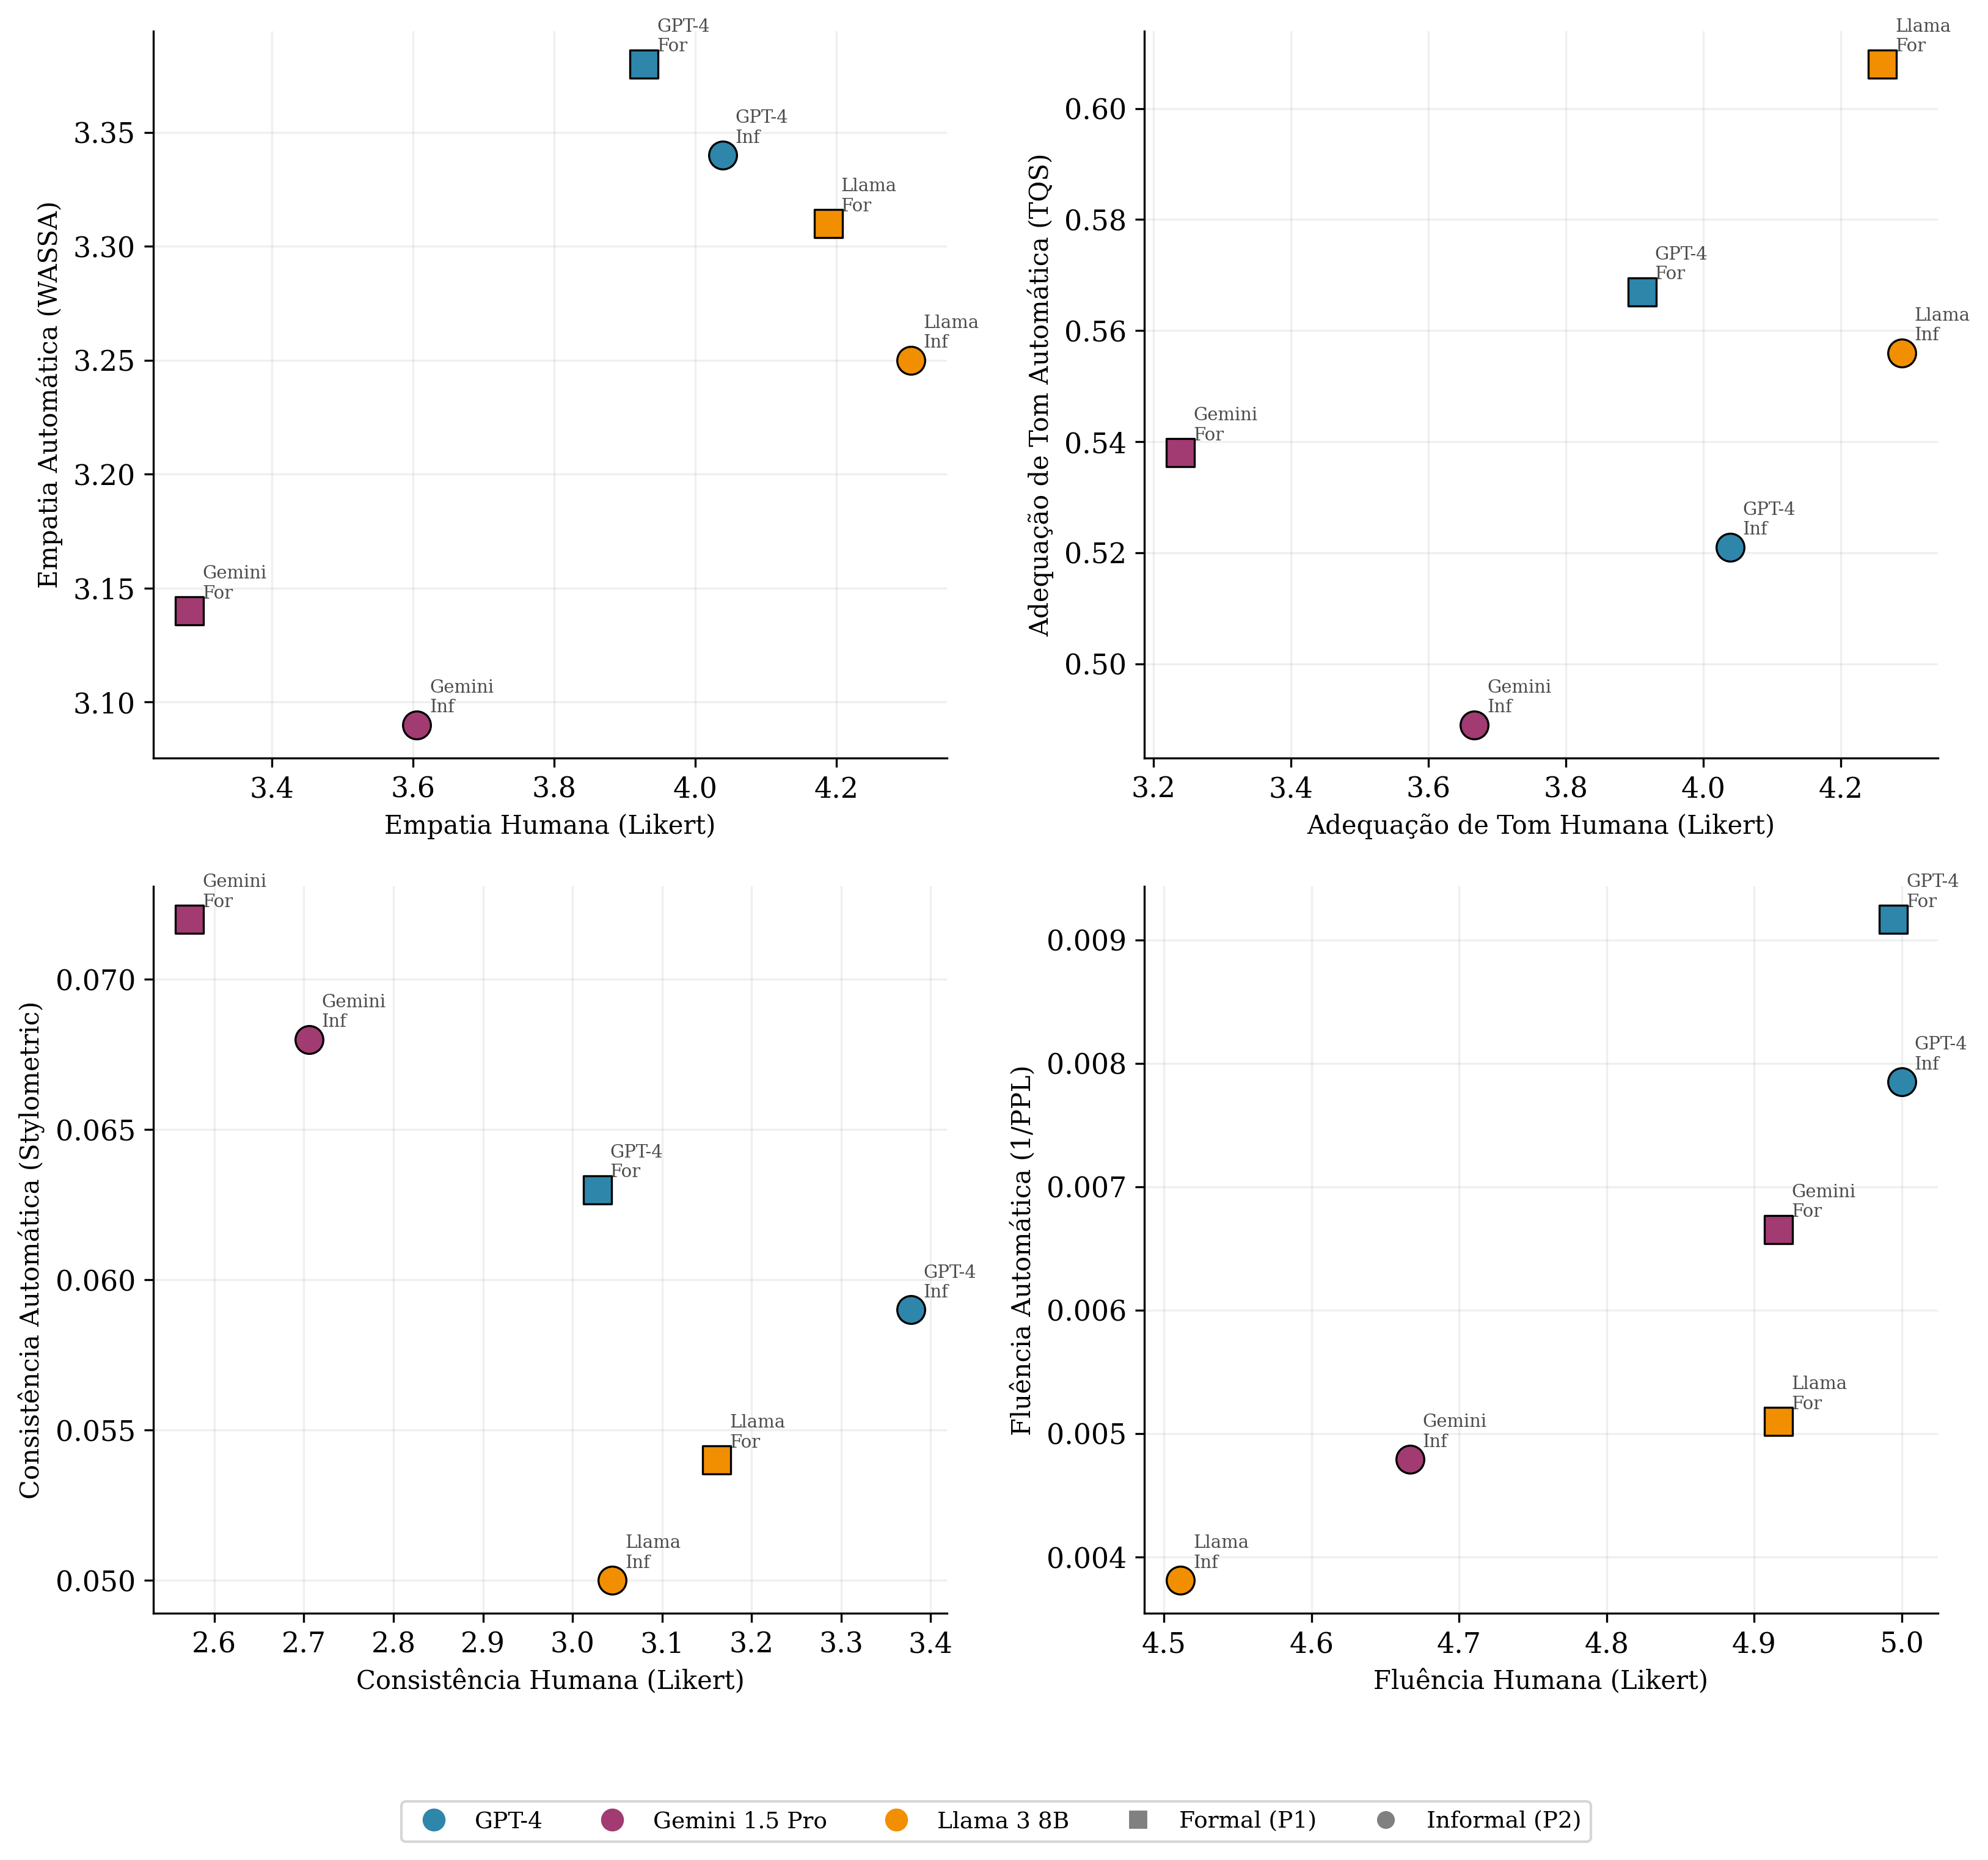
\includegraphics[width=0.9\textwidth]{img/dispersao_humano_automatico.png}
\caption{Dispersão entre avaliações humana (eixo X) e automática (eixo Y) por modelo e persona. Quadrados representam a persona formal (P1), círculos a informal (P2). }
\label{fig:dispersao_humano_automatico}
\end{figure}

\subsubsection{Convergências}

Os rankings de \textit{adequação de tom} e \textit{fluência} são idênticos nas duas modalidades de avaliação. Na adequação de tom, tanto a avaliação humana quanto o ToneCal posicionam \textit{Llama 4} $>$ \textit{GPT-5.5} $>$ \textit{Gemini}, o que fortalece a validade dessa métrica como \textit{proxy} confiável. Na fluência, tanto a percepção humana quanto a perplexidade convergem no ranking \textit{GPT-5.5} $>$ \textit{Gemini} $>$ \textit{Llama 4}. Essas convergências sustentam a utilidade do ToneCal e da perplexidade como indicadores automáticos para suas respectivas dimensões.

\subsubsection{Divergências}

Na dimensão de \textit{empatia}, ocorre uma inversão no topo do ranking: os 15 avaliadores humanos classificam o cenário \textit{Llama 4} como o mais empático (4,247), enquanto a métrica WASSA posiciona o \textit{GPT-5.5} em primeiro lugar (3,360). Essa divergência é atribuível às limitações do modelo WASSA, treinado em inglês para o domínio de notícias, com compressão de escala acentuada (CV $= 4{,}91\%$) que limita seu poder discriminativo em português brasileiro no domínio de atendimento ao cliente.

A divergência mais expressiva ocorre na \textit{consistência de marca}: a avaliação humana posiciona \textit{GPT-5.5} como mais consistente (3,203), enquanto a similaridade estilométrica favorece o \textit{Gemini} (0,070), uma inversão completa de ranking. A estilometria mede similaridade superficial de estilo (léxico e sintaxe) com base nas 200 respostas originais do restaurante (100 do período \textit{before} e 100 do período \textit{after}), ao passo que os avaliadores humanos avaliam a adequação pragmática e contextual da resposta à identidade da marca.

\subsubsection{Viés de Registro Linguístico}

A inversão direcional do efeito de persona entre avaliação humana e métricas automáticas constitui um achado transversal relevante. Na avaliação humana, a persona informal (P2) recebe pontuações superiores em empatia, consistência de marca e adequação de tom para todos os modelos (Tabela~\ref{tab:modelo_persona}). Nas métricas automáticas, a persona formal (P1) é sistematicamente favorecida: WASSA (P1 $= 3{,}329$ vs.\ P2 $= 3{,}205$), ToneCal (P1 $= 0{,}555$ vs.\ P2 $= 0{,}538$) e perplexidade (P1 $= 128{,}4$ vs.\ P2 $= 223{,}1$). Essa inversão constitui evidência de que métricas automáticas baseadas em modelos de linguagem, treinados predominantemente em texto formal, apresentam viés compartilhado para registro formal, podendo conduzir a conclusões opostas às da percepção humana real.

\subsubsection{Natureza Aproximativa das Métricas Automáticas} 
Os achados de convergência parcial e divergência sistemática entre avaliação humana e métricas automáticas precisam ser interpretados à luz da \textit{natureza proxy} desses indicadores. As métricas \textit{Perplexidade}, \textit{ToneCal}, \textit{Writeprints} e \textit{WASSA}, ainda que cientificamente fundamentadas, constituem \textit{aproximações computacionais} de fenômenos linguísticos e pragmáticos complexos, e não verdades absolutas sobre a qualidade do texto avaliado. Cada métrica captura uma faceta operacionalizável de uma dimensão multidimensional da comunicação humana, definida pelas escolhas de modelagem, pelo corpus de treinamento e pelos pressupostos do método que a originou.

A \textbf{perplexidade} mede a probabilidade que um modelo de linguagem específico atribui a uma sequência textual. Como o \textit{GPT-2 PT-BR} foi pré-treinado em corpora majoritariamente compostos por texto formal, notícias jornalísticas, artigos enciclopédicos e literatura editada, suas estimativas de fluência tendem a favorecer respostas com sintaxe canônica, léxico padrão e estruturas oracionais previsíveis. Construções típicas do registro informal brasileiro (contrações, marcas de oralidade, sintaxe paratática) recebem, por essa razão, perplexidades sistematicamente mais altas, ainda que sejam percebidas pelos avaliadores humanos como mais naturais no contexto de atendimento ao cliente em redes sociais.
 
 O \textbf{ToneCal} opera sobre marcadores lexicais explícitos de cortesia, deferência e 
formalidade. A métrica é sensível a saudações formais, fórmulas de tratamento e uso do modo subjuntivo, elementos predominantemente associados ao registro formal. Por consequência, respostas que mobilizam empatia através de proximidade afetiva, acolhimento informal e linguagem coloquial podem receber pontuações inferiores, mesmo quando a percepção humana as classifica como mais adequadas ao contexto pragmático de uma resposta a um cliente. A métrica captura, portanto, polidez lexical de superfície, não adequação pragmática contextualizada.
 
O \textbf{modelo WASSA} foi treinado em \textit{datasets} anotados majoritariamente em inglês e originados de domínios jornalísticos. Ainda que sua arquitetura baseada em \textit{transformers} multilíngues permita transferência parcial para outras línguas e domínios, a representação interna do conceito de empatia que o modelo aprendeu está ancorada nos padrões lexicais e estruturais do material de treinamento. Aplicado a respostas em português brasileiro no domínio de \textit{review} de restaurantes, o modelo produz estimativas comparativamente úteis para diferenciar modelos e estratégias, mas com valores absolutos cuja calibração não pode ser presumida.

A \textbf{similaridade estilométrica} (\textit{Writeprints}) mensura a aproximação entre o perfil estilístico de uma resposta gerada e o de um corpus de referência humano (distribuição lexical, complexidade sintática, \textit{n-gramas} de caracteres, padrões de pontuação). A métrica é, por construção, agnóstica ao conteúdo semântico e à adequação pragmática: uma resposta pode espelhar fielmente o estilo da marca sem responder de forma apropriada ao comentário recebido, e o inverso também é possível. A divergência observada nesta dimensão (ranking estilométrico oposto ao ranking humano) ilustra com clareza essa limitação conceitual. A explicação unificadora para o padrão recorrente \textit{``métricas automáticas favorecem o formal, humanos preferem o acolhedor''} é, portanto, estrutural: todas as métricas adotadas dependem, direta ou indiretamente, de modelos de linguagem ou de corpora de referência cuja distribuição amostral pende para o registro formal. Esse \textit{viés compartilhado} não invalida as métricas, elas continuam fornecendo sinais comparativos consistentes e reprodutíveis, mas demarca o seu campo legítimo de aplicação: \textit{proxies} úteis para comparações relativas e triagem em larga escala, jamais substitutos da avaliação humana em decisões finais sobre qualidade comunicacional. Daí a centralidade metodológica da triangulação adotada neste estudo: a integração sistemática entre as duas modalidades é o que permite distinguir achados robustos (confirmados por ambas) de artefatos da medição automática (presentes apenas em uma).

\section{CONCLUSÕES}

\subsection{Síntese dos Resultados}

O achado central desta investigação é que \textit{não existe um modelo universalmente superior} em todas as dimensões avaliadas. A análise de 2.400 respostas geradas, com avaliação automática integral e avaliação humana em amostra estratificada de 72 itens por 15 avaliadores independentes e quatro métricas automáticas especializadas, revela um cenário de \textit{trade-offs} inerentes entre as dimensões de qualidade. O cenário do \textit{Llama 4} apresenta as maiores pontuações na percepção humana de empatia (4,247/5) e adequação de tom (4,275/5), enquanto o \textit{GPT-5.5} é superior em fluência (4,997/5) e consistência de marca (3,203/5). O \textit{Gemini 3.1} é consistentemente inferior em três das quatro dimensões humanas, com diferenças estatisticamente significativas confirmadas pelo teste de \textit{Kruskal-Wallis} ($p < 0{,}05$ em todas as dimensões). Esse resultado corrobora a perspectiva de avaliação holística de \citeonline{liang2023}, segundo a qual modelos de linguagem exibem perfis de competência heterogêneos que somente avaliações multidimensionais conseguem capturar adequadamente.

A estratégia \textit{zero-shot}, apoiada em descrições robustas de persona, tende a superar a \textit{few-shot} na percepção humana de empatia ($\Delta = +0{,}357$, $p = 0{,}074$) e adequação de tom ($\Delta = +0{,}387$) para todos os modelos testados, com efeito especialmente pronunciado no \textit{Gemini} ($\Delta > +0{,}65$). Embora o efeito global não atinja significância estatística convencional ($\alpha = 0{,}05$), a consistência direcional entre os três modelos sugere uma tendência substantiva. Exemplos \textit{few-shot} parecem restringir a expressividade dos modelos, gerando respostas percebidas como mais templáticas e menos empáticas. Esse achado contraria a expectativa usual de que exemplos demonstrativos melhoram o desempenho, sugerindo que, para tarefas que requerem expressividade e engajamento emocional, a instrução descritiva pode ser mais eficaz do que a demonstração por exemplos.

\subsection{Contribuição Metodológica}

A principal contribuição metodológica deste estudo é a proposição e validação empírica de um \textit{framework} de avaliação multidimensional que integra avaliação humana e métricas automáticas para a geração de texto em português brasileiro. Esse \textit{framework} combina quatro dimensões de avaliação humana (empatia, consistência de marca, adequação de tom e fluência) com quatro \textit{proxies} computacionais (WASSA, ToneCal, perplexidade GPT-2 e similaridade estilométrica), permitindo a triangulação sistemática entre percepção humana e medição automática.

A demonstração empírica de que essa triangulação é \textit{necessária}, e não apenas desejável, constitui um dos achados centrais do trabalho. As divergências sistemáticas entre avaliação humana e métricas automáticas seguem um padrão previsível: métricas treinadas predominantemente em texto formal favorecem sistematicamente o registro formal. A inversão direcional do efeito de persona (informal preferido por humanos; formal favorecido por métricas automáticas) é a evidência mais robusta desse viés compartilhado. Um estudo baseado exclusivamente em métricas automáticas teria chegado a conclusões parcialmente opostas às da percepção humana real, conforme alertado por \citeonline{howcroft2021} ao documentar os riscos de avaliações subdimensionadas em processamento de linguagem natural.

A concordância inter-avaliadores obtida ($\kappa = 0{,}76$--$0{,}86$; $\alpha = 0{,}82$--$0{,}94$; ICC $= 0{,}88$--$0{,}94$) atesta que a avaliação humana com painel diversificado é viável e reprodutível, reforçando seu papel como referência para a calibração de \textit{proxies} automáticos.

\subsection{Implicações Práticas}
\label{subsec:implicacoes}

Para aplicações comerciais no setor gastronômico, os resultados oferecem orientações concretas. A configuração \textit{zero-shot} com persona bem definida é indicada como \textit{default} operacional, dada a tendência consistente de superioridade em empatia e adequação de tom na avaliação humana. O \textit{GPT-5.5} oferece o menor risco e maior previsibilidade (menor variância entre cenários), sendo indicado quando fluência e profissionalismo são prioritários. O \textit{Llama 4} destaca-se como a opção mais indicada para aplicações em que a empatia percebida é o objetivo central.

A persona informal (acolhedora) é preferida pelos avaliadores humanos em três de quatro dimensões, indicando que, no contexto de SAC de restaurante, o tom acolhedor é mais valorizado do que o formal. Esse achado alinha-se com a evidência de \citeonline{rohden2024}, que demonstra o impacto positivo do tom empático de \textit{chatbots} na satisfação e no \textit{boca a boca} de consumidores. Do ponto de vista ético, a implantação de respostas automatizadas em larga escala deve considerar os riscos de representação, viés linguístico e geração de conteúdo potencialmente nocivo documentados por \citeonline{weidinger2021} e corroborados pela literatura sobre degeneração tóxica em modelos de linguagem~\cite{gehman2020, hartvigsen2022}, particularmente o viés para registro formal identificado neste estudo, que pode desfavorecer interações com públicos habituados ao registro informal. Reforça-se ainda que todos os comentários reais utilizados nesta pesquisa, bem como as capturas de tela apresentadas neste documento, passaram por procedimento sistemático de anonimização (remoção de nomes de usuários, identificadores de conta, fotografias de perfil e \textit{URLs} associadas), conforme detalhado na Seção~\ref{subsec:consideracoes_eticas}, em conformidade com os princípios da \textit{LGPD} (Lei n.\ 13.709/2018), assegurando que a reutilização do material no repositório do projeto preserve a privacidade dos autores originais dos comentários

 \subsection{Limitações do Estudo}
 
A despeito do rigor metodológico adotado, este estudo apresenta limitações que devem ser 
consideradas na interpretação dos resultados e que apontam caminhos para investigações futuras.
 
\subsection{Escala e representatividade do \textit{corpus}.}
 O \textit{Corpus de Origem} é composto por 200 comentários reais provenientes de um único estabelecimento (Coco Bambu Manaus). Embora a quantidade tenha sido cuidadosamente balanceada entre os períodos pré e pós-popularização das \textit{LLMs} e tenha gerado as 2.400 respostas que sustentam a análise, o tamanho amostral restringe a generalização dos achados para outras unidades, redes e contextos regionais. A coleta concentrada em um restaurante específico introduz, ainda, traços contextuais (tipo de culinária, perfil de clientela, padrão de queixas e elogios) que podem não se manifestar em outros segmentos do setor gastronômico.
 
 \subsection{Avaliação humana realizada em amostra estratificada.}
 A avaliação humana foi conduzida sobre uma amostra estratificada das 2.400 respostas geradas, com 15 avaliadores independentes cobrindo os 24 cenários experimentais. Embora a concordância inter-avaliadores obtida ($\kappa = 0{,}76$--$0{,}86$; $\alpha = 0{,}82$--$0{,}94$; ICC $=0{,}88$--$0{,}94$) atribua robustez aos resultados, a não-avaliação humana integral do \textit{Corpus Resultante} impede afirmações pontuais sobre respostas individuais, restringindo as conclusões ao nível agregado dos cenários.
 
 \subsection{Possível viés dos avaliadores.}
 Apesar dos cuidados adotados na seleção do painel e da aplicação de procedimentos de cegamento 
quanto ao modelo de origem de cada resposta, é razoável reconhecer que avaliações subjetivas em 
escala \textit{Likert} estão sujeitas a vieses individuais relacionados a preferências 
estilísticas, registro linguístico habitual e expectativas pessoais sobre comunicação 
institucional. A diversificação do painel mitiga, mas não elimina, esta fonte de variabilidade.
 
 \subsection{Limitações das métricas automáticas.}
 As métricas automáticas adotadas (Perplexidade, \textit{ToneCal}, \textit{Writeprints} e WASSA) 
constituem \textit{proxies} computacionais que aproximam dimensões complexas da qualidade textual,
 mas não substituem a avaliação humana. A Perplexidade reflete a probabilidade do texto sob um 
modelo de língua específico (\textit{GPT-2 PT-BR}), podendo favorecer padrões linguísticos 
próximos aos dados de seu pré-treinamento. O \textit{ToneCal} opera sobre marcadores lexicais de 
superfície, com sensibilidade maior a indicadores explícitos de polidez do que a nuances 
pragmáticas de tom implícito. O \textit{Writeprints} captura padrões estilométricos agregados, sem
 mensurar diretamente o conteúdo semântico ou a adequação contextual. O modelo \textit{WASSA}, 
originalmente treinado em inglês e em domínio jornalístico, é empregado como indicador comparativo
 entre modelos e estratégias, mais informativo para diferenças relativas do que para valores 
absolutos. Os achados deste estudo demonstram que a triangulação entre métricas e avaliação humana
 é necessária justamente por essas características.

 \subsection{Análise estatística e estrutura de dependência.}
 A análise inferencial deste estudo apoiou-se em testes não paramétricos clássicos 
(\textit{Kruskal-Wallis} para efeito global e \textit{Mann-Whitney U} para comparações pareadas), 
adequados à natureza ordinal das pontuações \textit{Likert}. Reconhece-se, entretanto, três 
limitações analíticas que apontam direções para refinamentos futuros. \textit{Primeiro}, as 
comparações pareadas foram reportadas com $p$-valores não corrigidos para comparações múltiplas; 
embora a magnitude e a consistência direcional dos efeitos reforcem a robustez dos achados 
principais, a aplicação de correções como \textit{Bonferroni} ou \textit{Benjamini-Hochberg} 
(\textit{FDR}) tornaria a inferência mais conservadora e é recomendada em estudos futuros. 
\textit{Segundo}, o estudo reporta diferenças médias ($\Delta$) e $p$-valores, mas não tamanhos de
 efeito padronizados (e.g., $\epsilon^2$ para \textit{Kruskal-Wallis}, $r$ de 
\textit{rank-biserial} para \textit{Mann-Whitney U}) nem intervalos de confiança, indicadores que 
ampliariam a interpretação prática da magnitude das diferenças observadas, especialmente em uma 
amostra moderada. \textit{Terceiro}, a estrutura dos dados apresenta dependências hierárquicas: 
cada avaliador avaliou múltiplas respostas, cada comentário do \textit{Corpus de Origem} originou 
respostas em múltiplos modelos, personas e estratégias, e cada resposta foi avaliada por múltiplos
 juízes. Essa estrutura de medidas repetidas e agrupamento múltiplo viola formalmente o 
pressuposto de independência das observações dos testes empregados. Modelos de efeitos mistos 
(\textit{linear mixed-effects models}) ou modelos cumulativos para variáveis ordinais 
(\textit{cumulative link mixed models}), com efeitos aleatórios para avaliador, comentário e 
modelo, constituem extensões naturais para trabalhos subsequentes, permitindo decompor a variância
 atribuível a cada fonte e produzir estimativas mais precisas dos efeitos fixos de interesse.
 
 \subsection{Generalização restrita ao domínio gastronômico.}
 O desenho experimental foi orientado ao contexto de respostas a comentários de restaurantes, com 
personas, instruções e exemplos calibrados para esse domínio. As conclusões sobre superioridade de
 estratégias de \textit{prompting}, comportamento dos modelos e adequação das métricas refletem 
essa especificidade. A transferência dos resultados para outros domínios de atendimento ao cliente
 (varejo, hotelaria, serviços financeiros, saúde) requer validação empírica adicional, dado que 
cada contexto impõe expectativas próprias de tom, formalidade e densidade informacional.
 
 \subsection{Possível influência de IA no período pós-popularização das \textit{LLMs}.}
 Embora a separação temporal do \textit{Corpus de Origem} (pré e pós 30 de novembro de 2022) tenha
 sido estabelecida justamente para mitigar a contaminação por respostas geradas por IA, não é 
possível assegurar, para o subconjunto pós-popularização, que todas as respostas humanas tenham 
sido elaboradas sem qualquer assistência de ferramentas generativas. Esta possibilidade afeta, em 
particular, o perfil estilométrico de referência utilizado na métrica de Similaridade 
Estilométrica (\textit{Writeprints}), composto a partir do conjunto completo das 200 respostas 
originais. Trabalhos futuros podem investigar essa influência restringindo a referência 
estritamente ao período pré-2022, ou desenvolvendo procedimentos automatizados de detecção de 
texto gerado por IA aplicados ao corpus de referência.
 
 \subsection{Configuração de geração e estabilidade dos modelos.}
 Os experimentos foram conduzidos com temperatura fixa ($T = 0{,}7$) e parâmetros de 
\textit{decoding} padrão das respectivas implementações, de modo a preservar o comportamento 
nativo de cada arquitetura. Variações sistemáticas desses parâmetros (e.g., \textit{top-p}, 
\textit{top-k}, \textit{frequency penalty}) podem alterar o equilíbrio entre criatividade e 
consistência das respostas. Adicionalmente, os modelos avaliados são produtos em evolução 
contínua: atualizações de versão por parte dos provedores podem introduzir mudanças 
comportamentais não controláveis externamente, o que torna a comparação entre modelos uma 
fotografia válida para a janela temporal em que os experimentos foram conduzidos.


%------------------------------------------------------

%------------BIBLIOGRAFIA---------------------
%\newpage
%\providecommand*{\refname}{}
%\renewcommand*{\refname}{\begin{center}\textit{REFERÊNCIAS}\end{center}}
%\newpage
%\vspace*{4cm}
%\pagestyle{empty}
%\pagestyle{myheadings}
%\addcontentsline{toc}{section}{REFERÊNCIAS}

\newpage
\providecommand*{\refname}{}
\renewcommand*{\refname}{\begin{center}\textit{REFERÊNCIAS}\end{center}}
\newpage
%\vspace*{4cm}
\pagestyle{empty}
\pagestyle{myheadings}
\addcontentsline{toc}{section}{REFERÊNCIAS}

%\bibliographystyle{sbc/sbc}
\bibliography{sbc_monografia}



% ---------------- INÍCIO DOS APÊNDICES ----------------


\newpage
\appendix % <--- Este comando inicia a área de apêndices
\renewcommand{\thesection}{\Alph{section}}
% Apêndice A
\section{Repositório do Projeto}
\label{apendice:repositorio}

O código-fonte desenvolvido para este trabalho, incluindo os arquivos de engenharia de \textit{prompts}, geração de respostas e avaliação automática (cálculo de métricas de fluência, ToneCal, similaridade estilométrica e empatia percebida), está disponível publicamente no seguinte repositório \textit{Git}:

\begin{center}
    \url{https://github.com/danilobsilv/llm_automatic_response_gen}
\end{center}

\section{Formulário de Avaliação Humana}
\label{apendice:formulario_completo}

Este apêndice apresenta a versão integral do formulário utilizado para a coleta dos dados qualitativos junto aos avaliadores, gerado via \textit{Google Forms}.

\includepdf[pages={1-3}, scale=0.85, pagecommand={}]{formulario_avaliacao.pdf}


% ---------------- FIM DOS APÊNDICES ----------------

\end{document}
